\part{Applications of Ch-bonding}
\cmpd*{m2pb}
\cmpd*{ebs-rhs-2py}
\cmpd*{ebs-ebs-2py}

\begin{refsection}

\chapter{Thermal rearrangement of a Ch-bonded solvate}
\label{sec:thermal-conversion}

This chapter was published in Cryst. Eng. Comm., 26 May 2020, and was originally titled \emph{Thermal conversion of a pyridine solvate to a de-solvate facilitated by rearrangement of chalcogen bonds. The solvate and non-solvate structures of N-(2-nitro-4-(3-oxobenzo[\emph{d}][1,2]selenazol-2(3\emph{H})-yl)phenyl)picolinamide.}\autocite{Fellowes2020a}. \footnote{Compound numbering, section titles, and terminology have been updated to fit this thesis.}

\section{Abstract}
The pyridine solvate of benzisoselenazolinone \cmpd{ebs-nitroamide-2py}$\cdot$pyridine is characterised by planar sheets of the benzisoselenazolinone \cmpd{ebs-nitroamide-2py} pierced by channels of pyridine molecules at an angle of 133\degree, the pyridine molecules are held in place by \ce{N\cdots Se} chalcogen bonding to the isoselenazolinone moiety.
These channels, which extend through the structure to the surface of the crystal, provide a means for escape of pyridine from the lattice when the crystal is heated to ca. 100\degree C.
Upon loss of the pyridine from these channels the remaining molecules undergo rearrangement to fill the space and in doing so the \ce{N\cdots Se} chalcogen bond in \cmpd{ebs-nitroamide-2py}$\cdot$pyridine is replaced by a \ce{C=O\cdots Se} chalcogen bond to give the non solvate \cmpd{ebs-nitroamide-2py}(ex.DMF).
The geometry of the chalcogen bond requires that the two benzisoselenazolinone ring systems which are essentially coplanar in \cmpd{ebs-nitroamide-2py}$\cdot$pyridine twist by an angle of 138\degree~resulting in the formation of highly corrugated sheets in the non solvate.

\section{Introduction}
Chalcogen bonding (Ch-bonding) is an attractive non-covalent interaction between a Lewis base and a chalcogen atom bearing an electron withdrawing substituent (X) (\cref{fig:ch-bonding});\autocite{Vogel2019,Bleiholder2006,Garrett2015a} it is directional and has a strength similar to hydrogen bonding.
Chalcogen bonding has applications in fields as diverse as medicinal chemistry,\autocite{Beno2015,Clark2007,Hudson2016,Iwaoka2002,Reid2014} anion sensing,\autocite{Lim2017,Garrett2016,Borissov2019} materials chemistry,\autocite{Biot2018} supramolecular chemistry,\autocite{Chen2018,Ho2016,Gleiter2018,Bleiholder2006,Huynh2017,Gleiter2003} and catalysis.\autocite{Wang2020}
In medicinal chemistry the chalcogen bond is considered as an isostere to \ce{N-H\cdots A} hydrogen bonding (\cref{fig:ch-bonding}), this property is currently being exploited in the development of new pharmaceuticals.

\begin{figure}
    \centering
    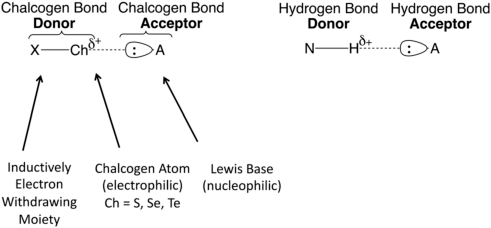
\includegraphics[width=0.8\linewidth]{Figures/ch-bonding.pdf}
    \caption{Chalcogen bonding model, and similarity to H-bonding.}
    \label{fig:ch-bonding}
\end{figure}

The mechanism of chalcogen bonding is believed to involve both electrostatic and orbital interaction components with dispersion being a lesser contributor.
The electrostatic component involves attraction between the Lewis base and a positively charged $\sigma$-hole which is generated along the extension of the \ce{Ch-X} bond due to polarisation of the bonding orbital, while the orbital  interaction component involves mixing between the occupied lone pair orbital of the Lewis base and the vacant $\sigma^{\star}_{\mathrm{Ch-X}}$ bond on the chalcogen, both these interactions account for the directionality of this interaction to different extents.
Whereas the electrostatic $\sigma$-hole interaction is believed to be the main contributor to the closely related halogen bonding interactions,\autocite{Prasang2009,Sarwar2010,Beale2013,Aakeroy2013,Goud2016,Stone2013} significant lengthening of the \ce{Ch-X} bond observed in the crystal structures of a number of chalcogen bonded systems is suggestive of a significant charge-transfer component to this interaction.\autocite{Fellowes2019,Pascoe2017}

\section{Results and discussion}
As part of our efforts towards a chalcogen-bonding based DNA minor-groove binding agent we required the benzisoselenazolinone \cmpd{ebs-nitroamide-2py}, which we proposed to cyclise to the benzimidazole-substituted  benzisoselenazolinone \cmpd{ebs-rhs-2py}, an analog to the Hoechst-type DNA-binding bisbenzimadazoles.\autocite{Loewe1974,Pjura1987,Martin2004}

\subsection{Synthesis}
The benzisoselenazolinone \cmpd{ebs-nitroamide-2py} was prepared from the diselenide \cmpd{diselenide} by conversion to the bis-electrophilic selenium reagent \cmpd{dichloride},\autocite{Lesser1924} followed by condensation with 2-nitro-1,4-benzenediamine to give the benzisoselenazolinone \cmpd{ebs-nitroaniline}, which was then coupled to picolinic acid via a Yamaguchi intermediate (\cref{sch:ebs-synthesis2}).

\begin{scheme}
\replacecmpd{diselenide}
\replacecmpd{dichloride}
\replacecmpd{ebs-nitroaniline}
\replacecmpd{ebs-nitroamide-2py}
\replacecmpd{ebs-rhs-2py}
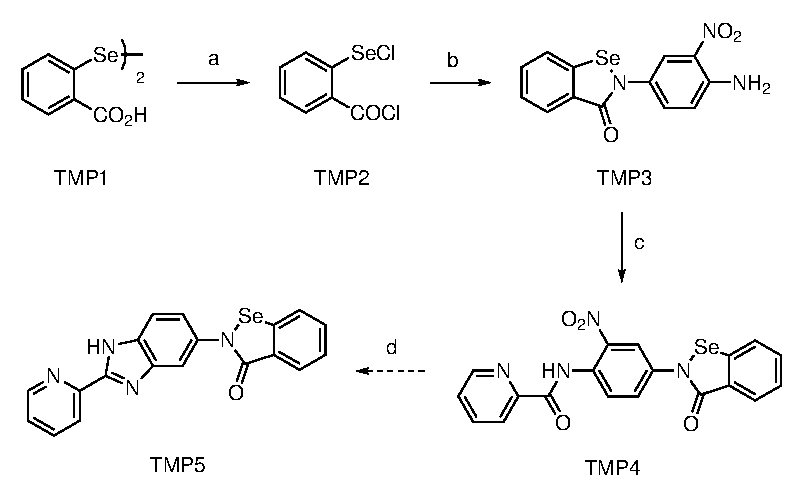
\includegraphics[scale=0.74]{Figures/ebs-synthesis3.eps}
\caption[Synthesis of precursor \refcmpd{ebs-nitroamide-2py}.]{Synthesis of precursor \refcmpd{ebs-nitroamide-2py}. a) \ce{SOCl2}, b) 2-nitro-1,4-benzenediamine, \ce{Et3N}, THF, c) Picolinic acid, TCBC/DMAP, \ce{Et3N}, d) [H], \ce{H+}.}
\label{sch:ebs-synthesis2}
\end{scheme}

\subsection{Structural characterisation}
Benzisoselenazoline \cmpd{ebs-nitroamide-2py} was found to be of low solubility in most organic solvents, but very small orange needles were obtained from slow evaporation from dimethylformamide.
The crystal structure obtained using data collected at the Australian Synchrotron was that of a non-solvate form, referred to herein as \cmpd{ebs-nitroamide-2py}(ex.DMF) in the orthorhombic space group Pbca.
A thermal ellipsoid plot for \cmpd{ebs-nitroamide-2py}(ex.DMF) is presented in \cref{fig:ebs-nitroamide-2py-dmf-xtal}.

\begin{figure}
    \centering
    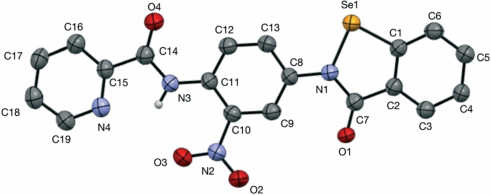
\includegraphics[width=0.8\linewidth]{Figures/ebs-nitroamide-2py-dmf-xtal.pdf}
    \caption[Thermal ellipsoid plot of \refcmpd{ebs-nitroamide-2py}(ex.DMF).]{Thermal ellipsoid plot of \refcmpd{ebs-nitroamide-2py}(ex.DMF). Ellipsoids are at the 50\% probability level.}
    \label{fig:ebs-nitroamide-2py-dmf-xtal}
\end{figure}

The crystal packing in \cmpd{ebs-nitroamide-2py}(ex.DMF) is characterised a number of non-covalent interactions including $\pi$-stacking which forms columns extending down the \emph{b} axis between molecules of \cmpd{ebs-nitroamide-2py} related by the \emph{b} glide plane (\cref{fig:ebs-nitroamide-2py-packing}).
The planes defined by the central aromatic ring C8-C13 are inclined at an angle 10.3(2)\degree~to the adjacent $\pi$-stacked molecule, with a centroid (C8-C13) plane distance of 3.414(4)~\AA~and a centroid–centroid distance of 3.786(4)~\AA~representing a slip distance of 1.636~\AA.

\begin{figure}
    \centering
    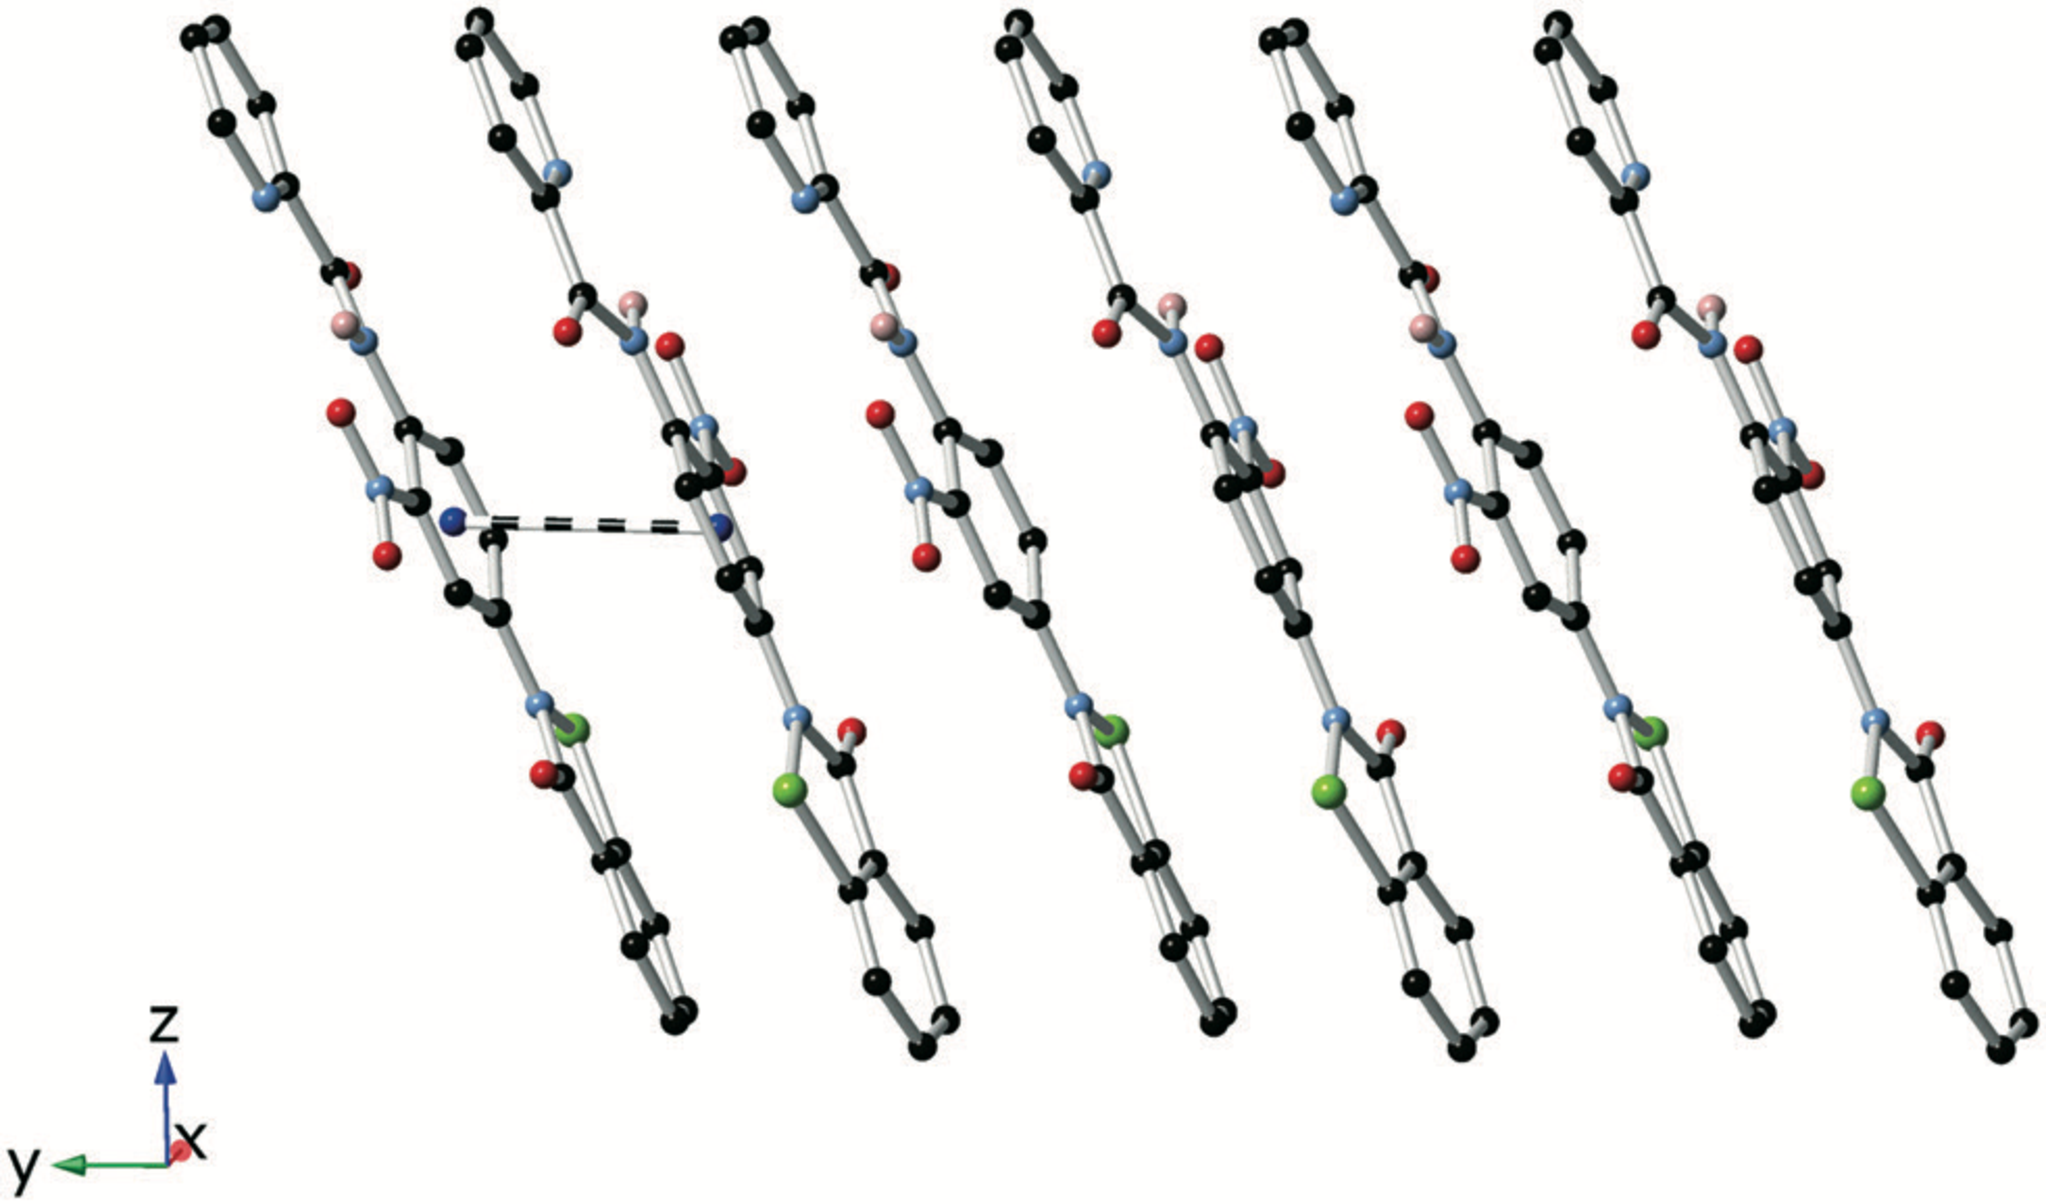
\includegraphics[width=0.8\linewidth]{Figures/ebs-nitroamide-2py-packing.pdf}
    \caption[Offset $\pi$-stacking of \refcmpd{ebs-nitroamide-2py}(ex.DMF) extending down the \emph{b}-axis.]{Offset $\pi$-stacking of \refcmpd{ebs-nitroamide-2py}(ex.DMF) extending down the \emph{b}-axis. The centroid-centroid distance is 3.786(4)~\AA.}
    \label{fig:ebs-nitroamide-2py-packing}
\end{figure}

Adjacent $\pi$-stacked columns are held together by chalcogen bonding interactions between the isoselenazolinone amide carbonyl oxygen and the selenium atom in the heterocyclic ring forming chains generated by the \emph{a}-glide plane extending down the \emph{a}-axis.
The \ce{O\cdots Se} distance is 2.659(3)~\AA~and the \ce{O\cdots Se-N} angle is 173.6(2)\degree.
The angle between the planes defined by the benzisoselenazolinone rings in the chalcogen bonded pairs is 138.8\degree~a coplanar arrangement is presumably disfavoured as this would result in severe steric clashes with the C5 of the benzisoselenazolinone ring.
Similar \ce{O\cdots Se} chalcogen bonding interactions have been observed in other benzisoselenazolinone derivatives related to the drug ebselen with comparable geometries.\autocite{Fellowes2019,Thomas2015,Bhabak2007,Piatek1995}
The \ce{N{3}-H{3}} group which is flanked by the pyridine nitrogen and the nitro group engages in intramolecular \ce{N-H\cdots N} and \ce{N-H\cdots O} hydrogen bonds, but is not involved in any significant intermolecular interactions (\cref{fig:ebs-nitroamide-2py-o-se}, \cref{fig:ebs-nitroamide-2py-pi-stacking}, \cref{fig:ebs-nitroamide-2py-3d}).

\begin{figure}
    \centering
    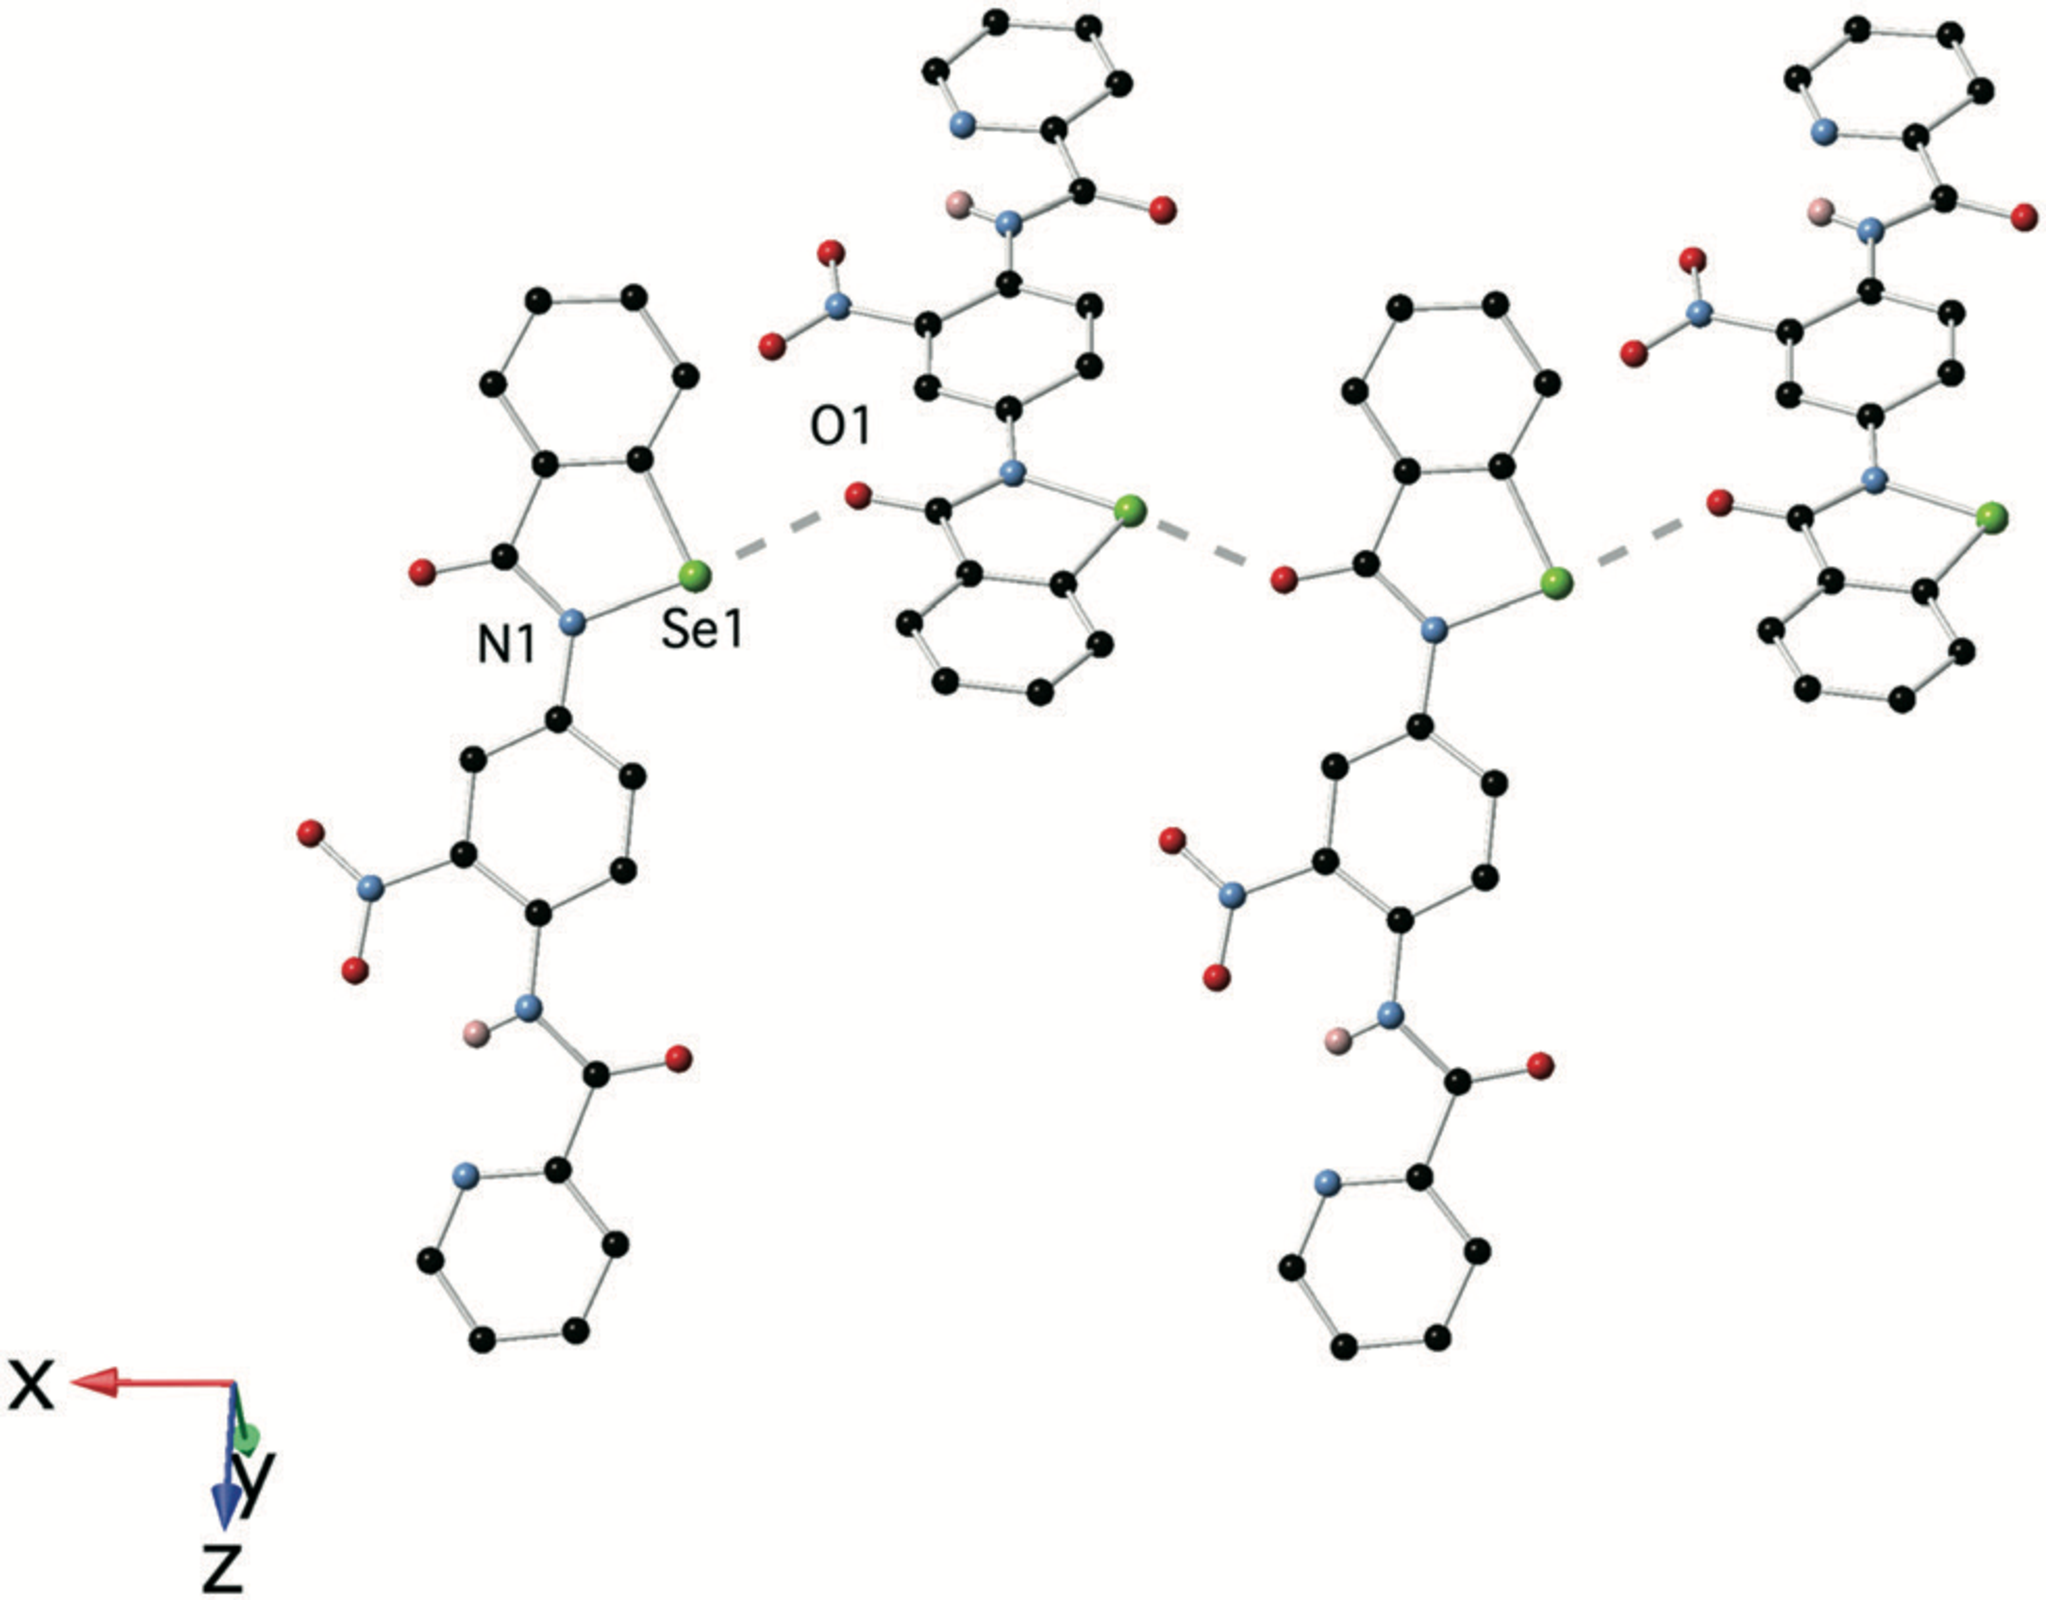
\includegraphics[width=0.8\linewidth]{Figures/ebs-nitroamide-2py-o-se.pdf}
    \caption{\ce{O\cdots Se} chalcogen bonding interactions in \refcmpd{ebs-nitroamide-2py}(ex.DMF).}
    \label{fig:ebs-nitroamide-2py-o-se}
\end{figure}

\begin{figure}
    \centering
    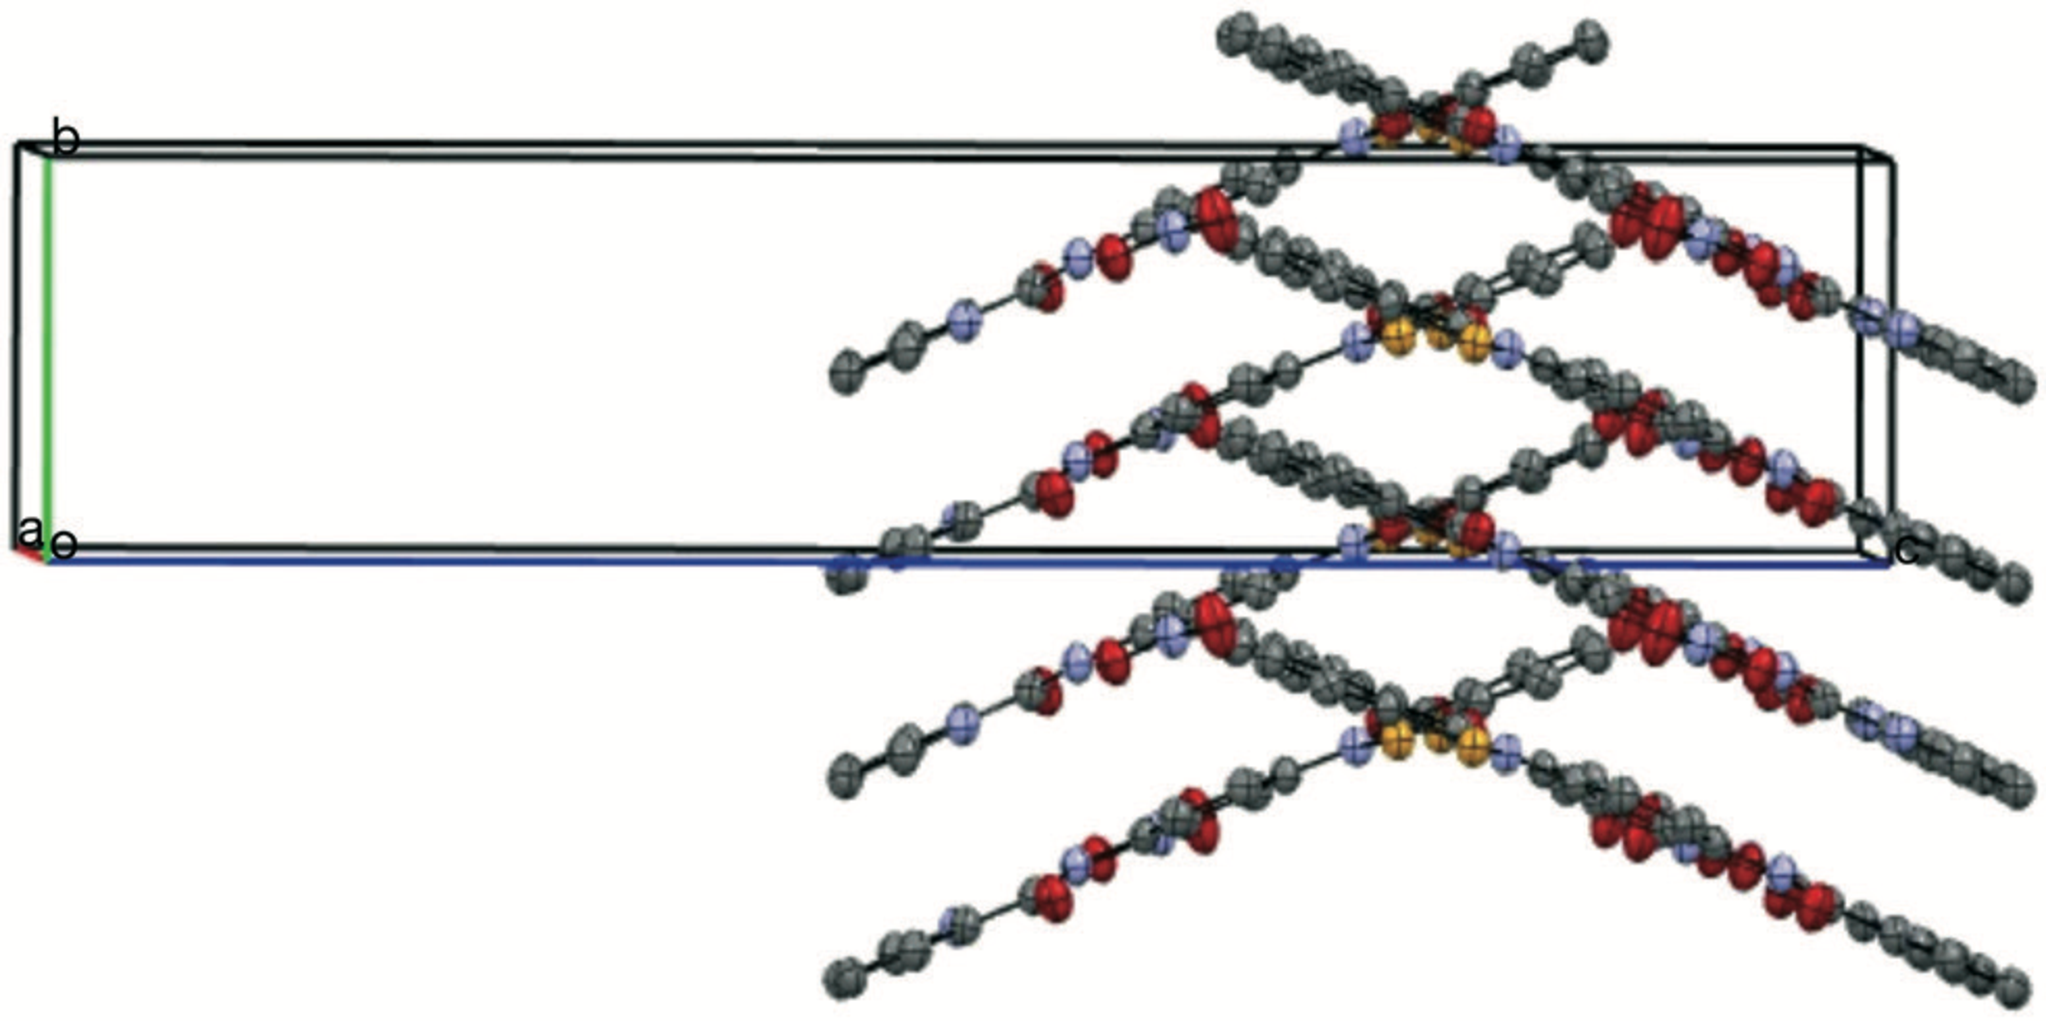
\includegraphics[width=0.8\linewidth]{Figures/ebs-nitroamide-2py-pi-stacking.pdf}
    \caption[2-D layers of \refcmpd{ebs-nitroamide-2py}(ex.DMF).]{2-D layers of \refcmpd{ebs-nitroamide-2py}(ex.DMF) $\pi$-stacking extends along the \emph{b}-axis while the \ce{Se\cdots O} chalcogen bond interactions extend down the \emph{a}-axis.}
    \label{fig:ebs-nitroamide-2py-pi-stacking}
\end{figure}

\begin{figure}
    \centering
    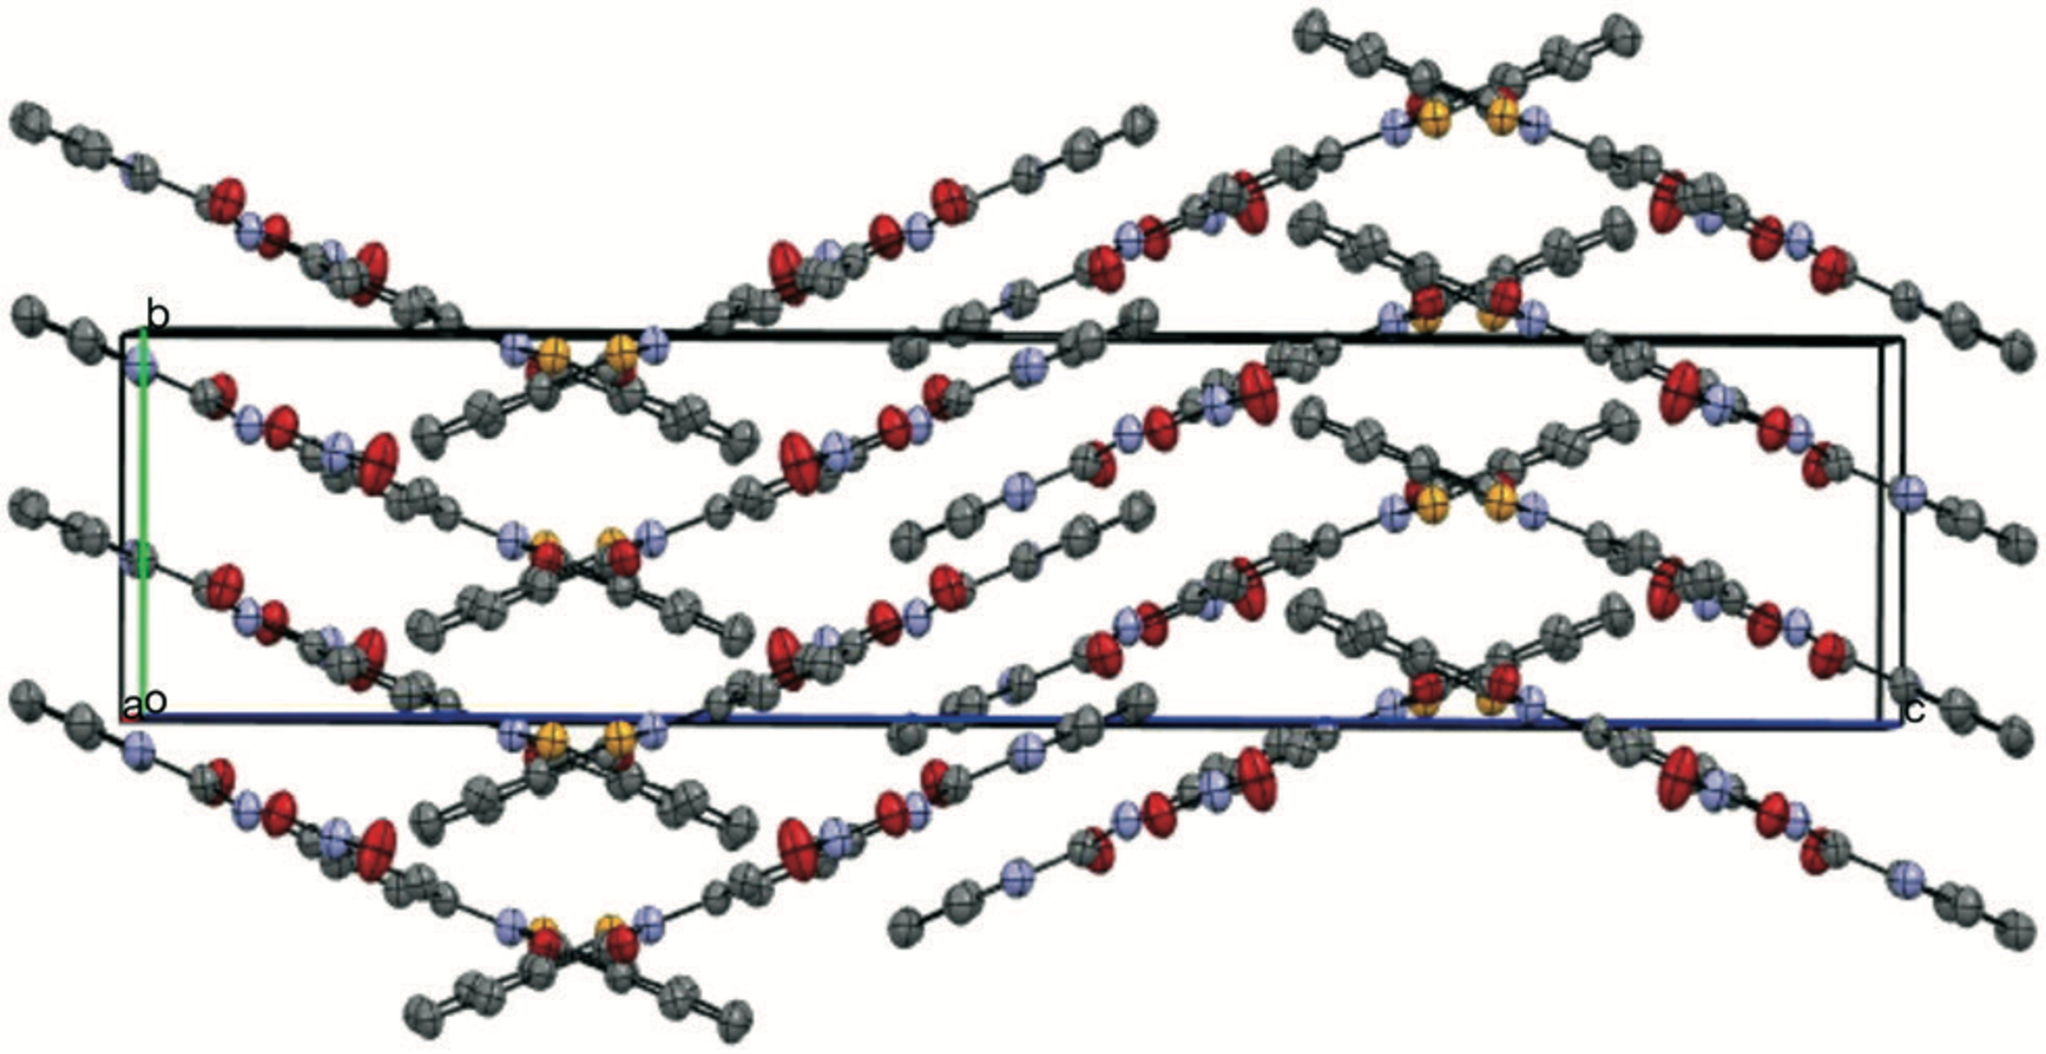
\includegraphics[width=0.8\linewidth]{Figures/ebs-nitroamide-2py-3d.pdf}
    \caption{Extension of the 2-D layers of \refcmpd{ebs-nitroamide-2py}(ex.DMF) into 3-D by van der Waals interactions.}
    \label{fig:ebs-nitroamide-2py-3d}
\end{figure}

The combination of the $\pi$-stacking and chalcogen bonding generates a 2-dimensional network lying parallel to the \emph{ab} plane.
These layers are extended into 3-dimensions by weaker Van-der Waals contacts between molecules related by the \emph{c} glide.

Crystallisation of benzisoselenazolinone \cmpd{ebs-nitroamide-2py} from pyridine gave rise to orange needles which were found to diffract well on the home-source diffractometer.
The structure solved in the monoclinic space group Pc and was found to be a pyridine solvate, herein labelled \cmpd{ebs-nitroamide-2py}$\cdot$pyridine.
The structure of \cmpd{ebs-nitroamide-2py}$\cdot$pyridine is presented in \cref{fig:ebs-nitroamide-2py-py-xtal} and shows that the pyridine solvate forms a \ce{N\cdots Se} chalcogen bond between the pyridine solvent molecule and the isoselenazolinone moiety.
The \ce{N{5}\cdots Se{1}} distance is 2.466(5)~\AA, the \ce{N{5}\cdots Se{1}-N{1}} angle is 173.2(2)\degree, and the angle between the plane of the coordinated pyridine ring and the benzisoselenazolinone ring is 89.2(1)\degree.
This geometry compares with previously reported chalcogen bonded adducts involving dimethylaminopyridine with simple benzisoselenazolinones.\autocite{Fellowes2019}
It is interesting to notethat upon formation of the chalcogen bond to pyridine, there is a significant lengthening of the \ce{Se{1}-N{1}} bond distance from 1.910(3)~\AA~in \cmpd{ebs-nitroamide-2py}(ex.DMF) to 1.945(5)~\AA~in \cmpd{ebs-nitroamide-2py}$\cdot$pyridine, which is consistent with the expected structural effects arising from the charge-transfer component of chalcogen-bonding.\autocite{Fellowes2019,Pascoe2017}

\begin{figure}
    \centering
    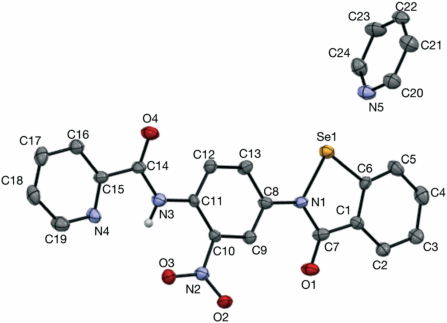
\includegraphics[width=0.8\linewidth]{Figures/ebs-nitroamide-2py-py-xtal.pdf}
    \caption[Thermal ellipsoid plot of \refcmpd{ebs-nitroamide-2py}$\cdot$pyridine.]{Thermal ellipsoid plot of \refcmpd{ebs-nitroamide-2py}$\cdot$pyridine. Ellipsoids are at the 50\% probability level.}
    \label{fig:ebs-nitroamide-2py-py-xtal}
\end{figure}

Molecules of \cmpd{ebs-nitroamide-2py} assemble into planar sheets lying parallel to the ($\bar{1} 0 4$) plane, the distance between these sheets as defined by the distance between the centroid of the atoms \ce{C{8}-C{13}} and the adjacent plane is 3.336~\AA~while the centroid-centroid distance is 4.973~\AA~representing a slippage of 3.688~\AA~(\cref{fig:ebs-nitroamide-2py-sheets-1}, \cref{fig:ebs-nitroamide-2py-sheets-2}).
The parallel sheets of molecules of \cmpd{ebs-nitroamide-2py} are pierced by channels of chalcogen bonded pyridine molecules which run parallel to the \emph{a}-axis at an angle of approximately 133\degree~to the plane.

\begin{figure}
    \centering
    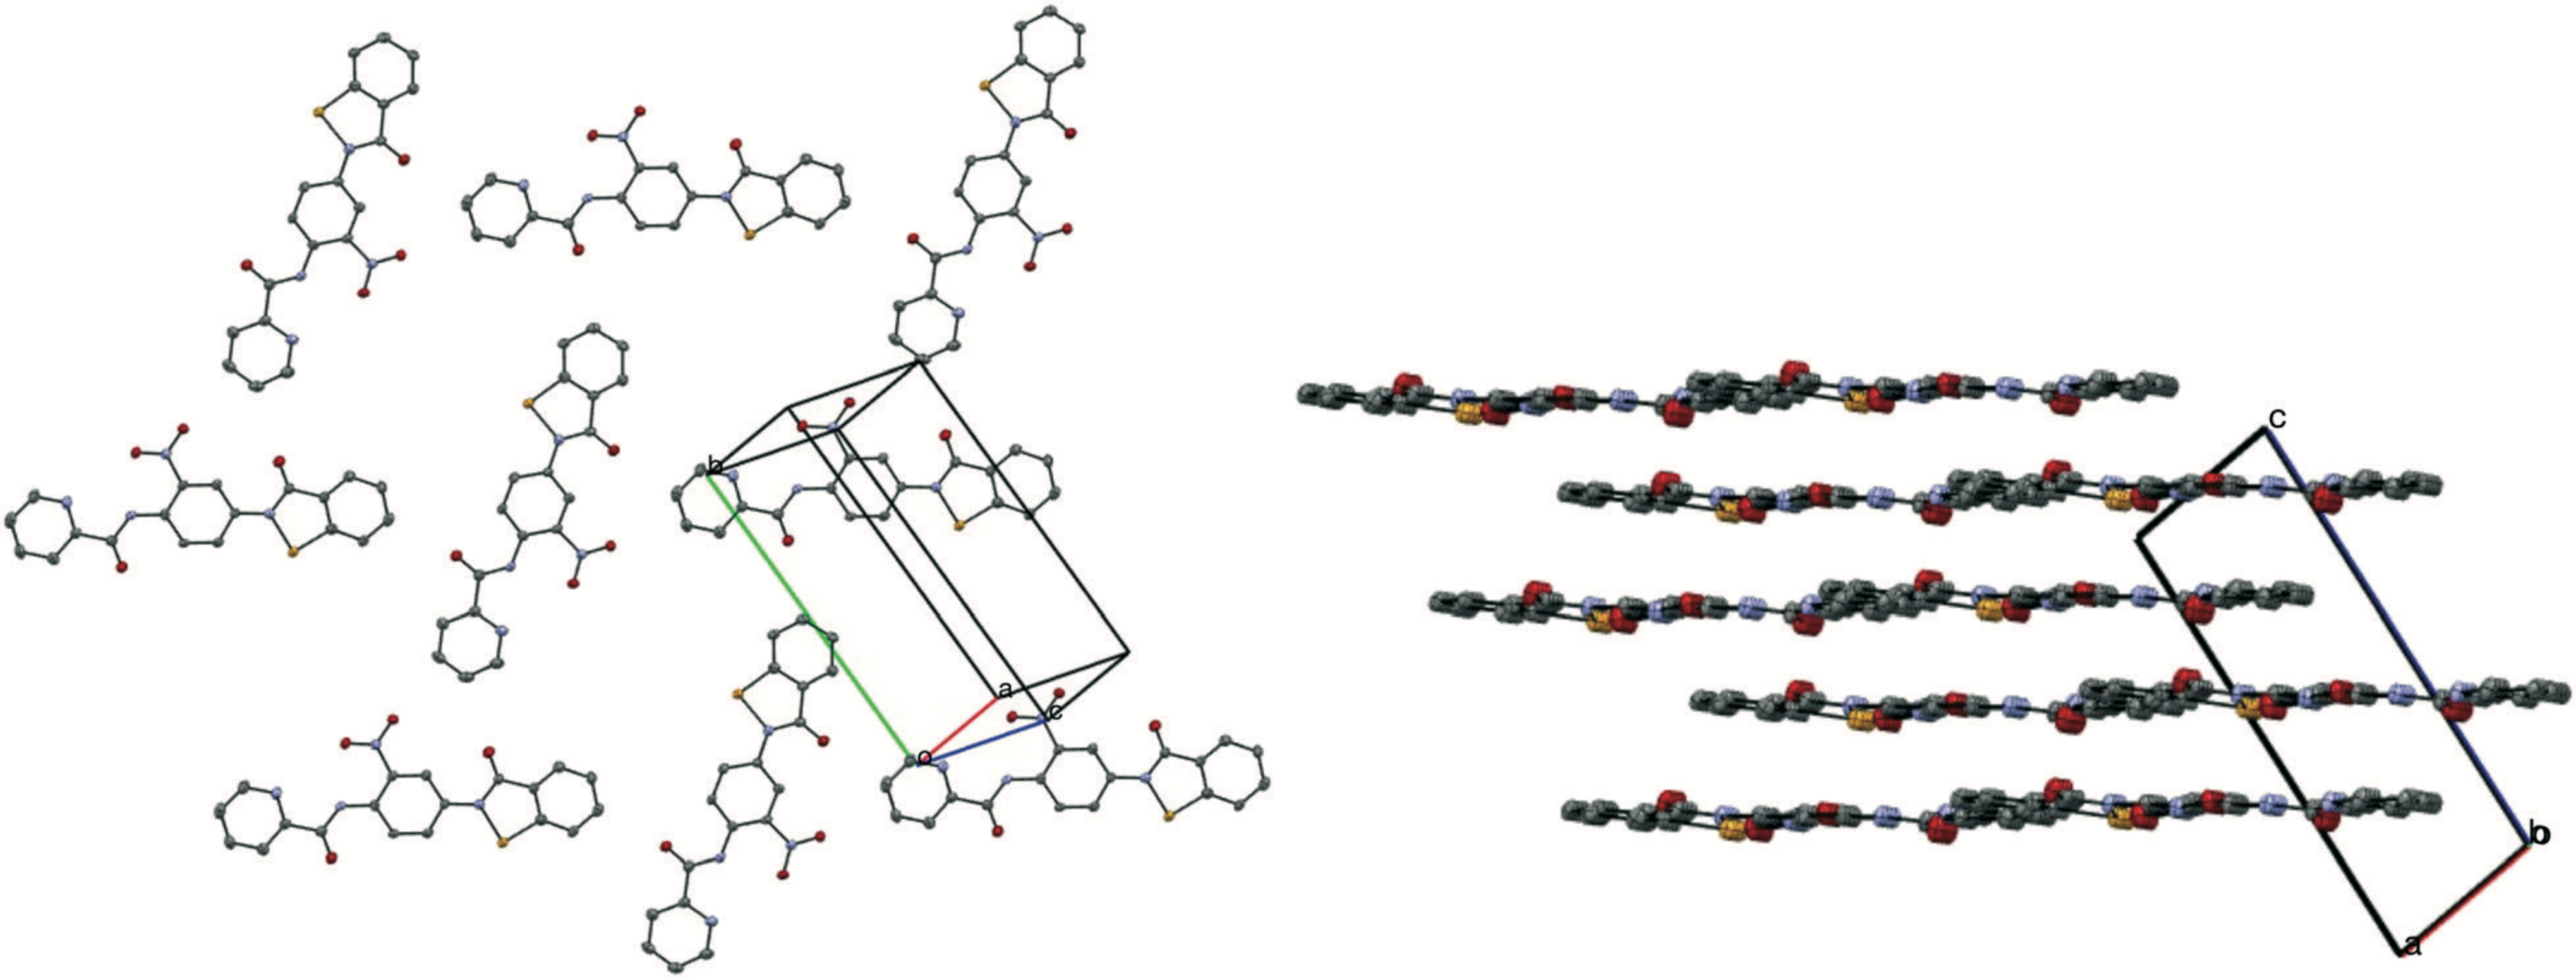
\includegraphics[width=0.8\linewidth]{Figures/ebs-nitroamide-2py-sheets-1.pdf}
    \caption[Sheets of compound \refcmpd{ebs-nitroamide-2py} viewed from orthogonal and parallel directions.]{Sheets of compound \refcmpd{ebs-nitroamide-2py} viewed from orthogonal and parallel directions. Pyridine solvate has been excluded.}
    \label{fig:ebs-nitroamide-2py-sheets-1}
\end{figure}

\begin{figure}
    \centering
    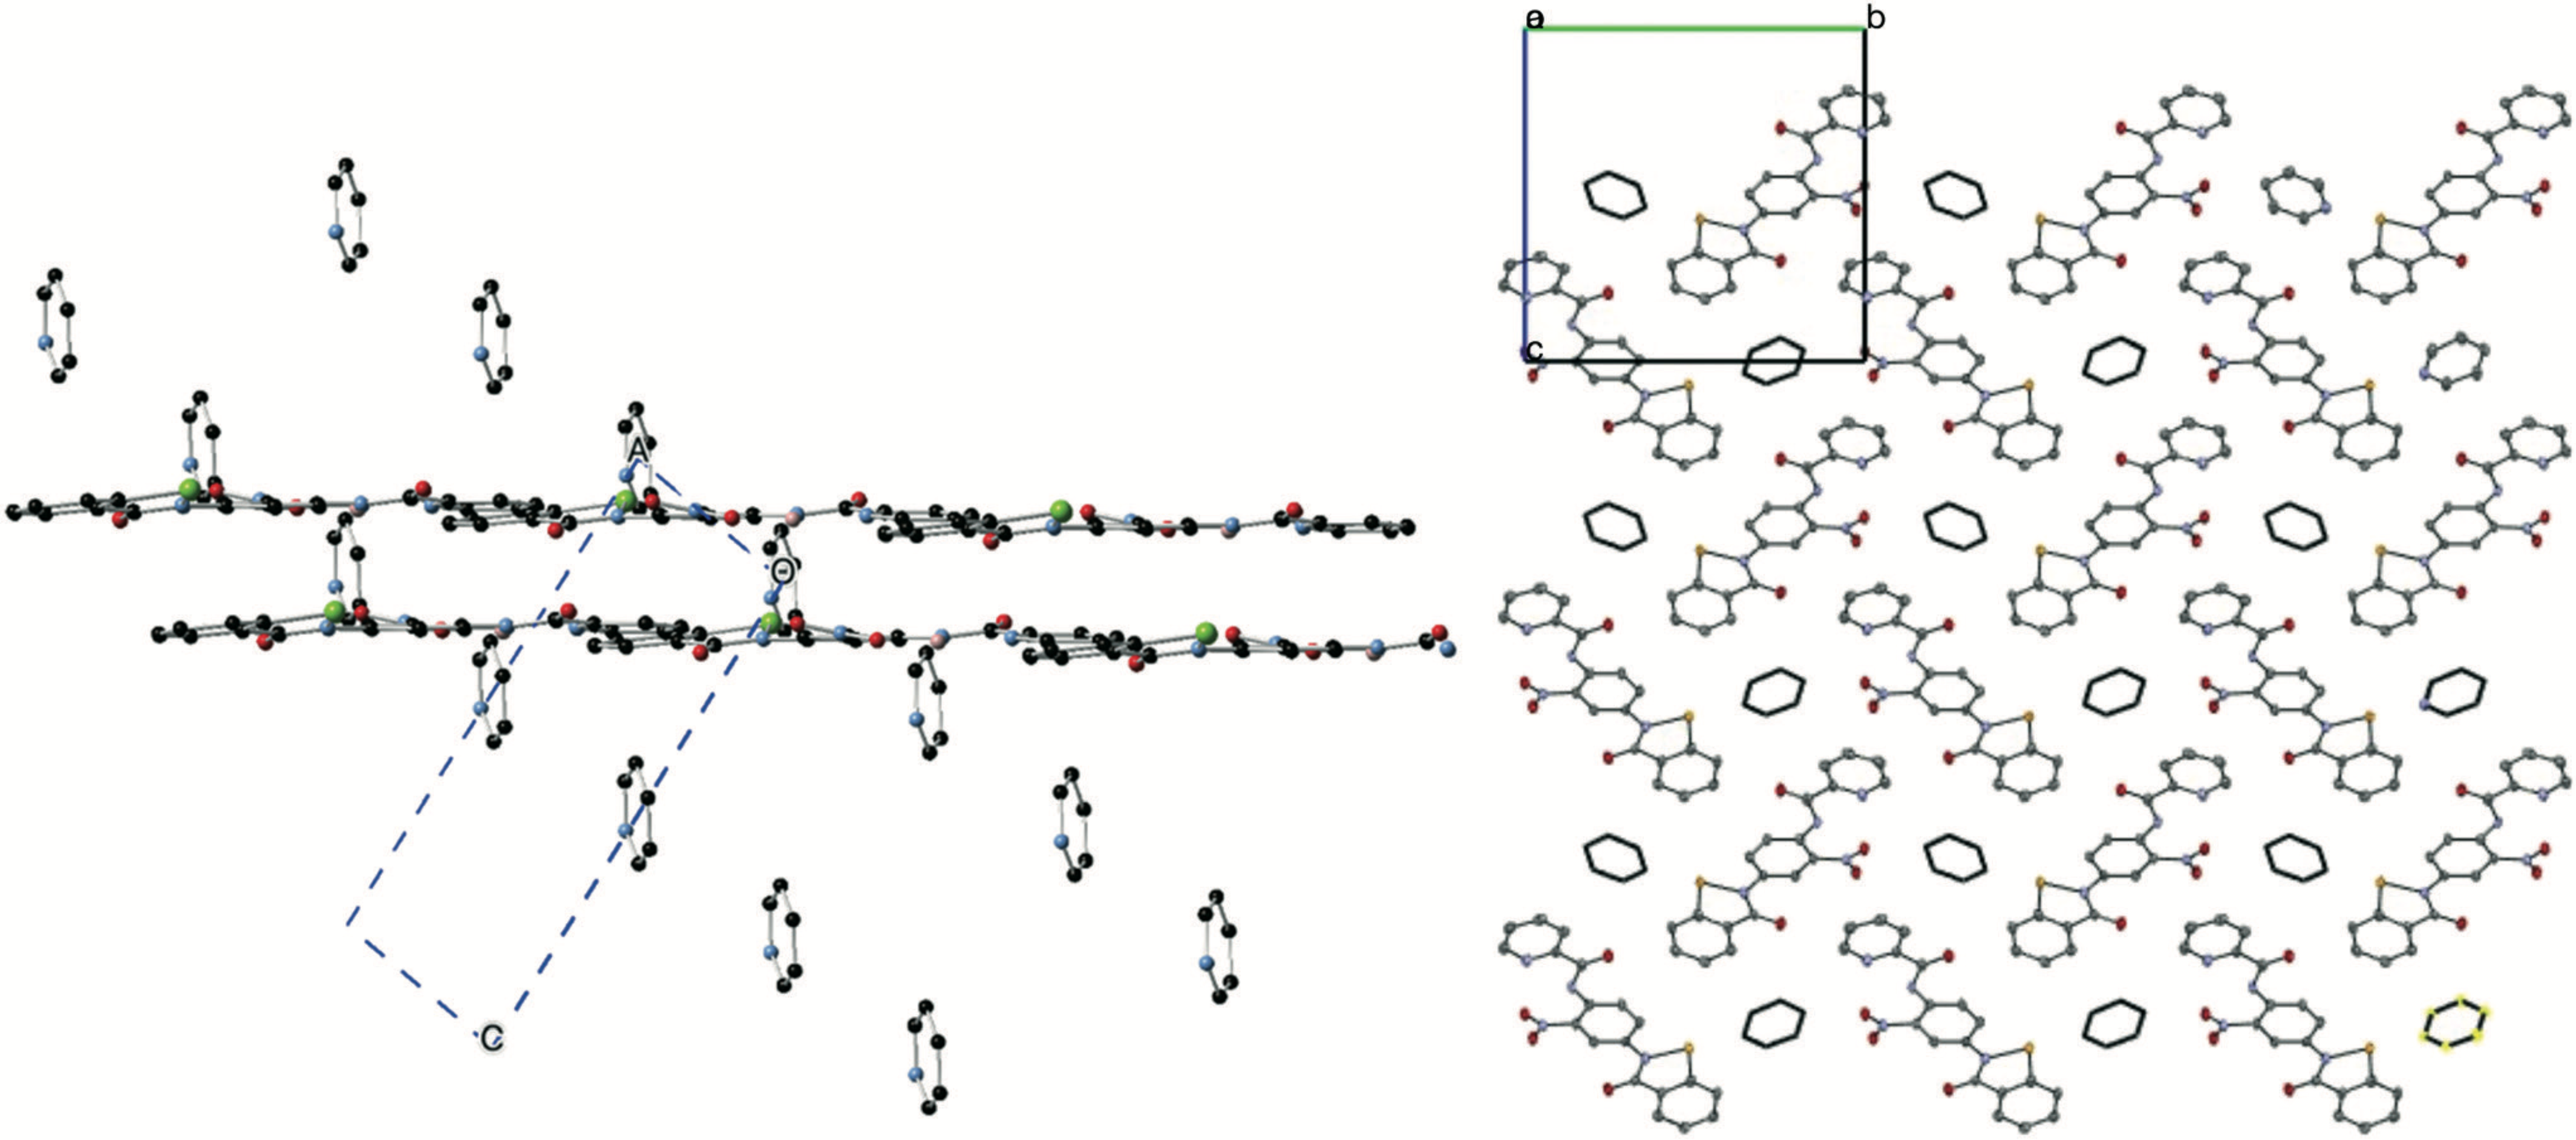
\includegraphics[width=0.8\linewidth]{Figures/ebs-nitroamide-2py-sheets-2.pdf}
    \caption[Two orthogonal views of parallel sheets of compound \refcmpd{ebs-nitroamide-2py}.]{Two orthogonal views of parallel sheets of compound \refcmpd{ebs-nitroamide-2py}, pierced by channels of pyridine molecules running parallel to the \emph{a}-axis.}
    \label{fig:ebs-nitroamide-2py-sheets-2}
\end{figure}

\subsection{Variable temperature studies}
Thermal gravimetric analysis of the pyridine solvate \cmpd{ebs-nitroamide-2py}$\cdot$pyridine was conducted on a Mettler TGA/SDTA851 apparatus in 40~$\mu$L aluminium crucibles.
A mass loss of 15.04\% occurred between 90--110\degree C corresponding to the loss of the pyridine solvate (calc. 15.26\%) followed by a second loss of 24.73\% between 300--360\degree C which is consistent with the loss of 121 a.m.u. very likely associated with the Pyr-C(O)NH moiety (\cref{fig:tga}).

\begin{figure}
    \centering
    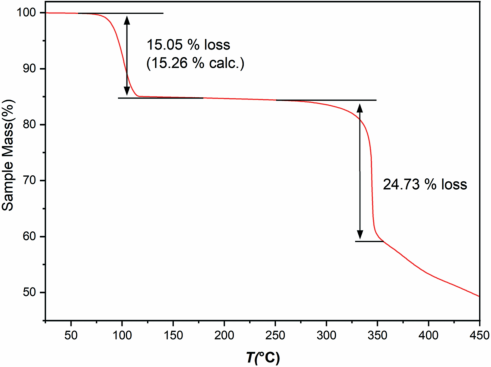
\includegraphics[width=0.8\linewidth]{Figures/tga.pdf}
    \caption{TGA analysis of \refcmpd{ebs-nitroamide-2py}$\cdot$pyridine.}
    \label{fig:tga}
\end{figure}

The observation that both the non-solvate \cmpd{ebs-nitroamide-2py}(ex.DMF) and \cmpd{ebs-nitroamide-2py}$\cdot$pyridine had the same melting point (experimental section below) intrigued us to establish whether desolvation of \cmpd{ebs-nitroamide-2py}$\cdot$pyridine which occurs between 90--120\degree C results in conversion to non-solvate \cmpd{ebs-nitroamide-2py}(ex.DMF).
Thus we carried out variable temperature powder X-ray diffraction measurements on \cmpd{ebs-nitroamide-2py}$\cdot$pyridine from -173\degree C to 117\degree C.
The resulting diffractograms are shown in \cref{fig:vt-pdx}.

\begin{figure}
    \centering
    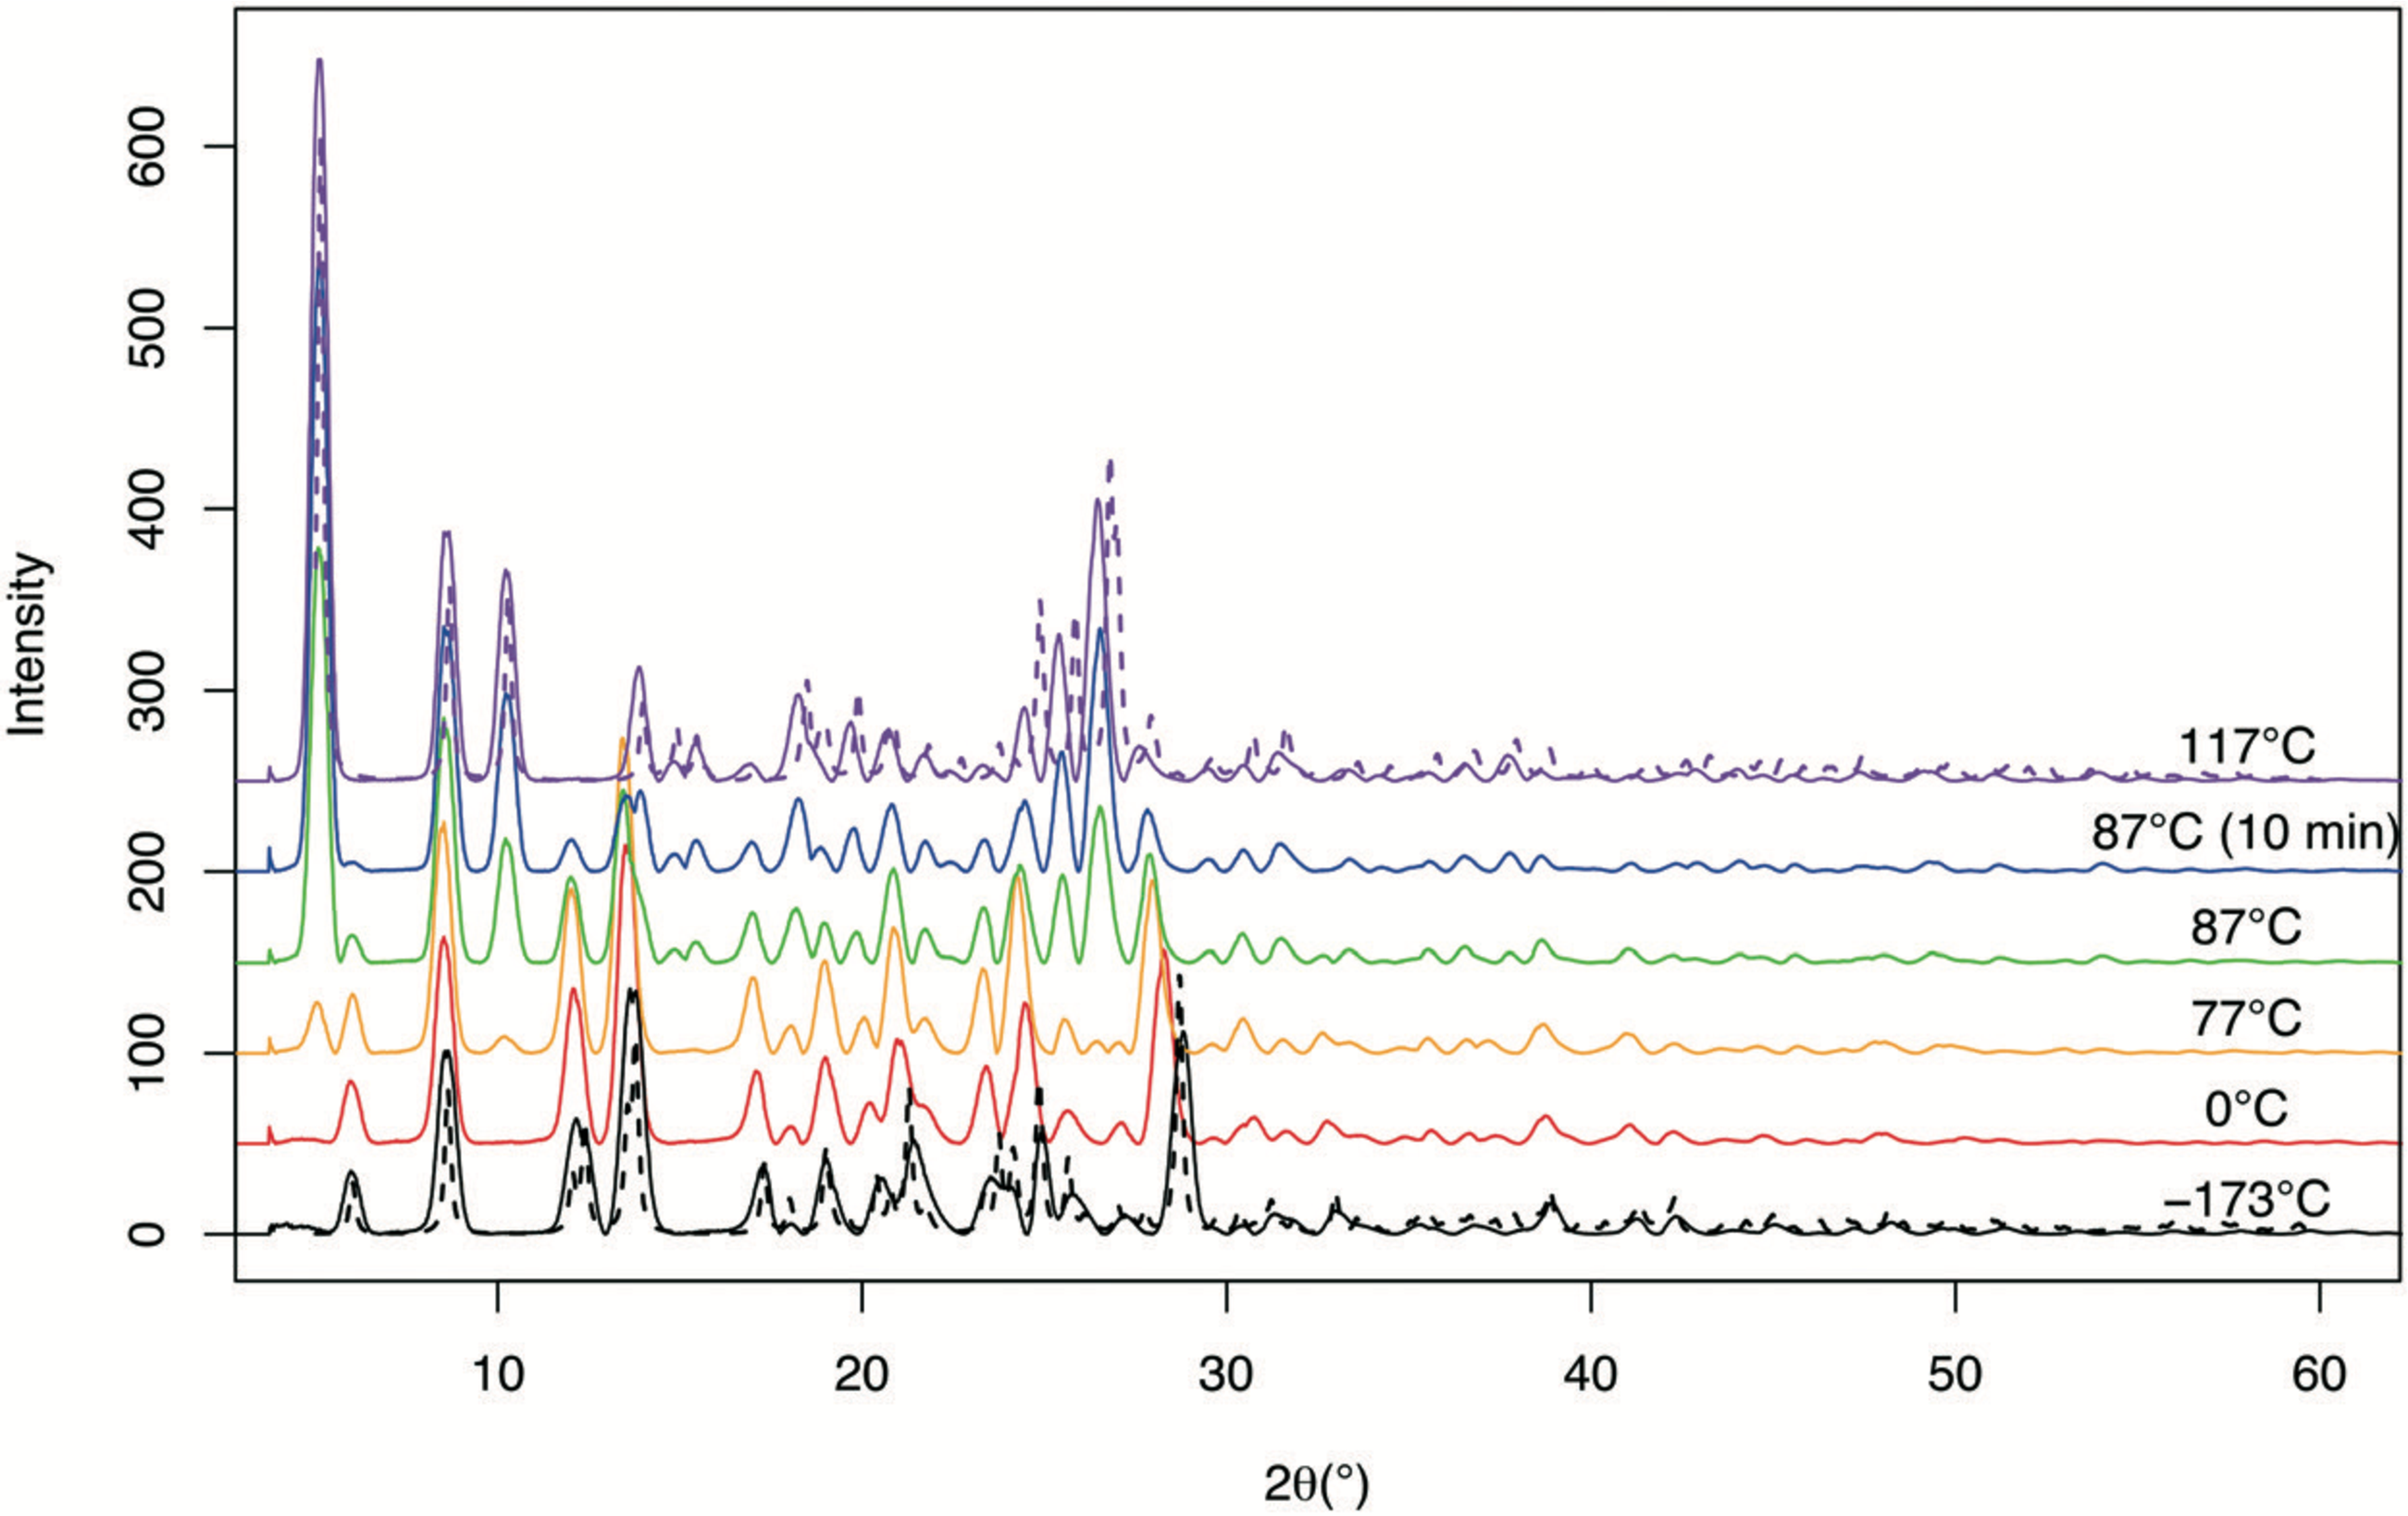
\includegraphics[width=\linewidth]{Figures/vt-pdx.pdf}
    \caption[Variable temperature powder XRD patterns from \refcmpd{ebs-nitroamide-2py}$\cdot$pyridine.]{Variable temperature powder XRD patterns from \refcmpd{ebs-nitroamide-2py}$\cdot$pyridine, calculated powder pattern for \refcmpd{ebs-nitroamide-2py}$\cdot$pyridine and \refcmpd{ebs-nitroamide-2py}(ex.DMF) are the dotted lines in the top and bottom traces respectively.}
    \label{fig:vt-pdx}
\end{figure}

From 87\degree C to 117\degree C when pyridine is known to be lost from the sample from the TGA analysis, there is a smooth change from one crystalline phase to another.
Furthermore comparison of the final diffractogram obtained after being kept at 117\degree C for 10 minutes very closely matches the calculated powder pattern for the non-solvate \cmpd{ebs-nitroamide-2py}(ex.DMF) suggesting the transformation from \cmpd{ebs-nitroamide-2py}$\cdot$pyridine into \cmpd{ebs-nitroamide-2py}(ex.DMF).
The same experiment was applied to a single crystal of \cmpd{ebs-nitroamide-2py}$\cdot$pyridine glued on a glass fibre to establish whether this transformation occurs from a single crystal of \cmpd{ebs-nitroamide-2py}$\cdot$pyridine to a single crystal of \cmpd{ebs-nitroamide-2py}(ex.DMF).
The crystal was heated to 90\degree C and heated at a rate of 0.5\degree C per minute to 120\degree C.
While there was a steady decrease in the intensity of the reflections for \cmpd{ebs-nitroamide-2py}$\cdot$pyridine, individual reflections consistent with a single crystal of \cmpd{ebs-nitroamide-2py}(ex.DMF) were not observed, but rather, there was the development of the powder pattern for \cmpd{ebs-nitroamide-2py}(ex.DMF).
Interestingly, throughout this transformation the crystal morphology did not appear to change significantly, but the final diffraction pattern was clearly that of a powder.
It is likely that the transformation (which must begin at the surface of the crystal) results in fragmentation of daughter crystals of the non-solvate, thus eroding away at the mother crystal.
We believe that a single crystal to single crystal transformation is very unlikely as collapsing of the channels containing the pyridine solvate would prevent complete desolvation.
A plausible mechanism for this interconversion likely involves replacement of the \ce{N\cdots Se} chalcogen bond in \cmpd{ebs-nitroamide-2py}$\cdot$pyridine, with a \ce{O\cdots Se} chalcogen bond involving the isoselenazolinone carbonyl group from a molecule in an adjacent layer which is at a distance of 12.051~\AA~(\cref{fig:ebs-nitroamide-2py-transformation}).

\begin{figure}
    \centering
    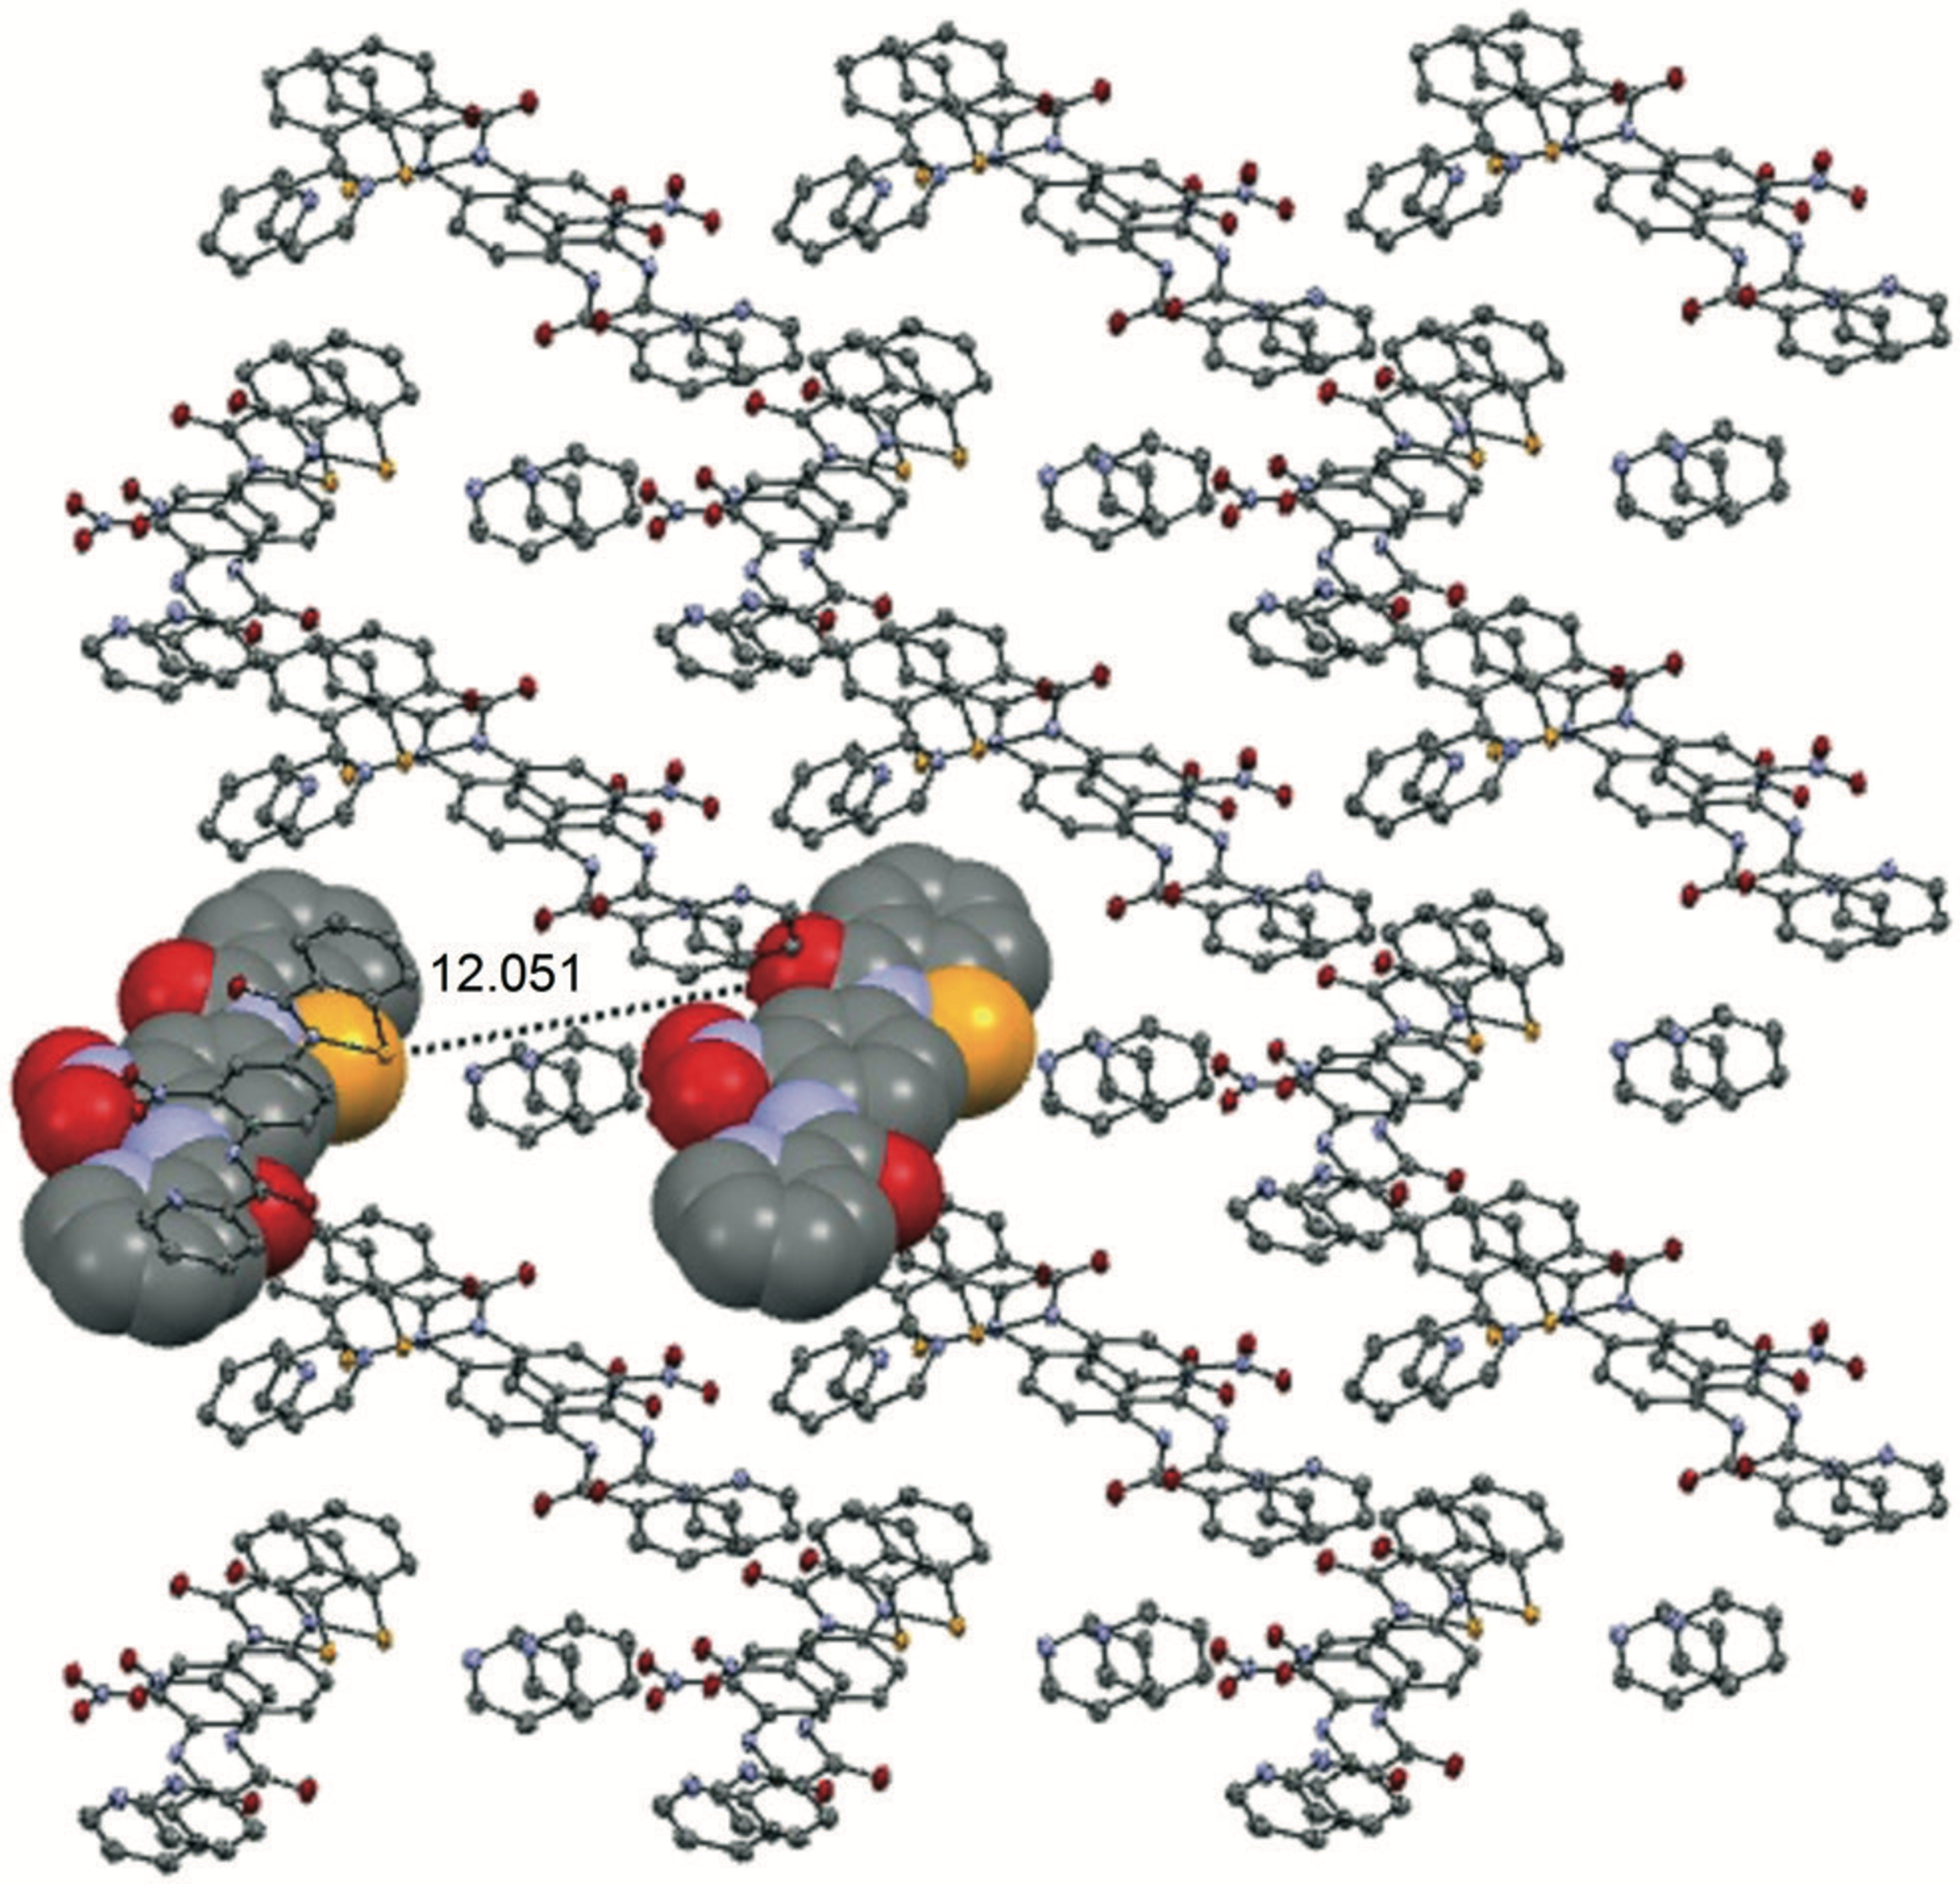
\includegraphics[width=0.8\linewidth]{Figures/ebs-nitroamide-2py-transformation.pdf}
    \caption[Rearrangement of Ch-bonds upon desolvation.]{Interlayer benzisoselenazolinones \refcmpd{ebs-nitroamide-2py} believed to form a \ce{O\cdots Se} chalcogen bond upon desolvation of \refcmpd{ebs-nitroamide-2py}$\cdot$pyridine.}
    \label{fig:ebs-nitroamide-2py-transformation}
\end{figure}

\section{Conclusion}
The structure of \cmpd{ebs-nitroamide-2py}$\cdot$pyridine is characterised by planar sheets of the benzisoselenazolinone \cmpd{ebs-nitroamide-2py} pierced by channels of pyridine molecules at an angle 133\degree, the pyridine molecules are held in place by \ce{N\cdots Se} chalcogen bonding to the isoselenazolinone moiety.
These channels which extend throughthe structure to the surface of the crystal provide a means for escape of pyridine from the lattice when the crystal is heated to ca. 100\degree C.
Upon loss of the pyridine from these channels the remaining molecules undergo rearrangement to fill the space and in doing so the \ce{N\cdots Se} chalcogen bond in \cmpd{ebs-nitroamide-2py}$\cdot$pyridine is replaced by a \ce{C=O\cdots Se} chalcogen bond to give the non solvate \cmpd{ebs-nitroamide-2py}(ex.DMF).
The geometry of the chalcogen bond requires that the two benzisoselenazolinone ring systems which are essentially coplanar in \cmpd{ebs-nitroamide-2py}$\cdot$pyridine twist by an angle of 138\degree~resulting in the formation of highly corrugated sheets in the non solvate.

\section{Experimental}
\subsection{Synthesis}
\subsubsection[Preparation of \refcmpd{ebs-nitroaniline}]{Preparation of 2-(4-amino-3-nitrophenyl)benzo[\emph{d}][1,2]-selenazol-3(2\emph{H})-one \refcmpd{ebs-nitroaniline}.}

Diselenide \cmpd{diselenide} (1.2025~g, 3.005~mmol) was dissolved in thionyl chloride (20~mL) and refluxed for 30~min, and the colour changed from purple to light yellow.
Excess thionyl chloride was removed \emph{in vacuo}, and the residue dissolved in anhydrous THF (50~mL).
To this was added a solution of 2-nitro-1,4-phenylenediamine (991.9~mg, 6.477~mmol) and triethylamine (dist. from \ce{CaH2}, 3~mL) in anhydrous THF (50~mL).
This mixture was stirred at room temperature for 18~h, then filtered, washing the precipitate with water, to afford 2-(4-amino-3-nitro-phenyl)benzo[\emph{d}][1,2]-selenazol-3(2\emph{H})-one \cmpd{ebs-nitroaniline} as a brick red solid (940~mg, 61\%, m.p. 300.8--302.0\degree C (DMF)).

{\footnotesize

\ce{^{1}H} NMR (400~MHz, \ce{\emph{d}6}-DMSO) $\delta$ ppm
7.08 (d, \emph{J} = 9.00~Hz, 1~H), 7.46 (t, \emph{J} = 7.43~Hz, 1~H), 7.55 (s, 2~H), 7.59--7.70 (m, 2~H), 7.86 (d, \emph{J} = 7.43~Hz, 1~H), 8.06 (d, \emph{J} = 7.83~Hz, 1~H), 8.12 (d, \emph{J} = 1.96~Hz, 1~H).

\ce{^{13}C} NMR (100~MHz, \ce{\emph{d}6}-DMSO) $\delta$ ppm
120.29, 121.49, 126.32, 126.71, 127.77, 128.31,128.45, 129.68, 132.66, 134.13, 139.33, 145.03, 165.70.

MS (ESI +ve) m/z 335.9882 (\ce{MH+}) \ce{C13H10N3O3Se+} requires 335.9881 ($\Delta$=0.3~ppm).
}

\subsubsection[Preparation of \refcmpd{ebs-nitroamide-2py}]{Preparation of N-(2-nitro-4-(3-oxobenzo[\emph{d}][1,2]selenazol-2(3\emph{H})-yl)\-phen\-yl) picolinamide \refcmpd{ebs-nitroamide-2py}.}

Picolinic acid (256.6~mg, 2.084~mmol) was dissolved in anhydrous THF (5~mL) and triethylamine (dist. from \ce{CaH2}, 1~mL), then trichlorobenzoylchloride (325~$\mu$L) was added and the mixture stirred for 10~min.
The above nitroaniline \cmpd{ebs-nitroaniline} (242.8~mg, 0.956~mmol) was then added, and the mixture stirred under argon for 24~h, during which time the dark red colour faded to give a yellow solution.
The mixture was tipped into water (100~mL) and filtered to afford a yellow precipitate, which was recrystallised from pyridine (50~mL) to give  N-(2-nitro-4-(3-oxobenzo[\emph{d}][1,2]selenazol-2(3\emph{H})-yl)phenyl)picolinamide \cmpd{ebs-nitroamide-2py} as yellow needles (93.2~mg, 20\%), m.p. 342.7--343.7\degree C (\emph{d}).
While recrystallization by slow evaporation from DMF gave small yellow needles m.p. 342--344\degree C (\emph{d}).

{\footnotesize

\ce{^{1}H} NMR (500~MHz, \ce{\emph{d}6}-DMSO) $\delta$ ppm
7.51 (t, \emph{J} = 7.40~Hz, 1~H) 7.66--7.83 (m, 1~H) 7.94 (d, \emph{J} = 7.63~Hz, 1~H) 8.04 (dd, \emph{J} = 7.8, 2.4~Hz, 1~H) 8.09--8.17 (m, 2~H) 8.23 (d, \emph{J} = 7.78~Hz, 1~H) 8.68 (d, \emph{J} = 2.44~Hz, 1~H) 8.73 (d, \emph{J} = 9.00~Hz, 1~H) 8.81 (d, \emph{J} = 4.43~Hz, 1~H) 12.22 (s, 1~H).

MS (ESI +ve) m/z 441.010 (\ce{MH+}) \ce{C19H13N4O4Se+} requires 441.0096 ($\Delta$=0.9~ppm).
}

\subsection{Crystallography}
Intensity data for \cmpd{ebs-nitroamide-2py}$\cdot$pyridine was collected on a Rigaku XtalLAB Synergy at 100.0(1)~K.
Data for \cmpd{ebs-nitroamide-2py}(ex.DMF) was collected on the MX1 beamline\autocite{Cowieson2015} at the Australian Synchrotron.
The temperature was maintained using an Oxford Cryostream cooling device.
The structures were solved by direct methods and difference Fourier synthesis.\autocite{Sheldrick2015}
Thermal ellipsoid plots were generated using the program Mercury\autocite{Macrae2008} integrated within the WINGX\autocite{Farrugia1999} suite of programs.
Other figures were obtained with both Mercury software and Crystal Maker software.

\subsubsection{Crystal data for \texorpdfstring{\refcmpd{ebs-nitroamide-2py}(ex.DMF)}{C19H12N4O4Se}}
\ce{C19H12N4O4Se}, \emph{M} = 439.29, \emph{T} = 100.0~K, $\lambda$ = 0.82656~\AA, orthorhombic, space group Pbca, \emph{a} = 12.652(3), \emph{b} = 7.5250(15), \emph{c} = 34.367(7)~\AA, \emph{V} = 3272.0(11)~\AA$^3$, \emph{Z} = 8, $D_c$ = 1.784~mg~M$^{-3}$, $\mu$ = 3.383~mm$^{-1}$, \emph{F}(000) = 1760, crystal size $0.05 \times 0.005 \times 0.005$~mm$^3$, 35758 reflections measured, $\theta_{\mathrm{max}}$ = 32.28\degree , 3282 independent reflections [R(int) = 0.0803], the final \emph{R} was 0.0601 [$I > 2\sigma(I)$, 2513 reflections] and $wR(F^2)$ was 0.1802 (all data), GOF 1.037.

\subsubsection{Crystal data for \texorpdfstring{\refcmpd{ebs-nitroamide-2py}$\cdot$pyridine}{C19H12N4O4Se.C5H5N}}
\ce{C19H12N4O4Se\cdot C5H5N}, \emph{M} = 518.39, \emph{T} = 100.0~K, $\lambda$ = 1.54184~\AA, monoclinic, space group Pc, \emph{a} = 4.9726(2), \emph{b} = 14.6836(5), \emph{c} = 14.4255(5)~\AA, $\beta$ = 98.154(4)\degree, \emph{V} = 1042.64(7) \AA$^3$, \emph{Z} = 2, $Dc$ = 1.651~mg~M$^{-3}$, $\mu$(Cu-K$\alpha$) = 2.829~mm$^{-1}$, \emph{F}(000) = 524, crystal size $0.12 \times 0.033 \times 0.026$~mm$^3$, 6794 reflections measured, $\theta_{\mathrm{max}}$ = 76.79\degree, 3132 independent reflections [R(int) = 0.0558], the final R was 0.0422 [$I > 2\sigma(I)$, 2977 data] and $wR(F^2)$ was 0.1107 (all data), GOF 1.098.

\section{Acknowledgements}
We gratefully acknowledge Sirtex Medical for funding and the Australian Synchrotron for beamtime via the Collaborative Access Program (proposal 13618b).
The Australian Research Council for Post Graduate Scholarships (TF and MPVK).

\printbibliography[heading=subbibliography]
\end{refsection}
%--------------------------------------------------------------------------------------------------%
\begin{refsection}

\chapter{Development of a Ch-bonding DNA binder}
\label{ch:dna-binder}

\section{Introduction}

\subsection{Cancer and treatment}
In Australia, cancer consistently ranks as one of the leading causes of death among all age groups. In 2015, lung cancer alone accounted for 8,466 deaths, which ranked only behind ischaemic heart disease (19,777), dementia (12,625), and cerebrovascular diseases (10,869).
If other cancers are included, the total number of deaths attributable to cancer is 1.5 times those caused by heart disease\autocite{abs2015}.

It has clear and serious consequences among families and communities, and also a wider economic price, costing Australia \$2 billion each year, of which the majority is spent on treatment\autocite{Mathers1998}.
Developing treatments for cancer has therefore attracted significant interest from the pharmaceutical industry, government, and the general public\autocite{Rankin2015}.

Cancer is not a single disease, but an umbrella term which encompasses many different types of malignancies.
The uniting theme among them is the uncontrolled and damaging division of cells.
Because of the diversity of diseases broadly termed ``cancer'', treatments are often difficult to develop and highly specific to one particular class\autocite{Hanahan2011}.

Some more general treatments for cancer exist.
These include surgery and radiation therapy.
While these treatments do have limitations (e.g. surgery is only viable for solid tumours), they are usually very effective, and are often combined with more specific therapies where appropriate.


\subsection{Radiation therapy}
Radiation therapy is one such general treatment for cancer.
A course of radiation therapy consists of a series of exposures to radiation (x-rays, generated electrically; $\gamma$-rays, generated by radioactive decay; or, less commonly, fermionic particles such as protons, neutrons or electrons), with the intention of damaging the DNA of the cancer cells beyond the cells' ability to repair, resulting in death of the cells and remission of the cancer\autocite{Ward1994}.
The mechanism of this damage is either direct, where a photon ejects an electron from the DNA polymer itself (via Compton scattering); or indirect, where other molecules (usually water) are ionised by the radiation, generating reactive oxygen species (ROS) such as \ce{^{$\cdot$}OH} and \ce{O_{2}^{-}}\autocite{Ward1988}.

If generated in the vicinity of the nucleus, these ROS may diffuse short distances and abstract electrons from DNA, causing damage to the DNA\autocite{Evans2004}.
Due to the minuscule volume occupied by DNA within the cell, indirect damage is the dominant mechanism in external beam radiotherapy\autocite{Ward1988}.

Damage to DNA can occur at the sugar-phosphate backbone or within the bases themselves, resulting in a range of fragmentation products or cross-linked adducts\autocite{Evans2004}.
Such products are not effective substrates for cellular processes such as DNA replication, so cell death usually occurs at the time of mitosis, if not before\autocite{Withers1992}.

Radiation therapy is targeted to inflict the greatest damage on cancer cells, while leaving healthy cells untouched.
In other words, the aim is to maximise therapeutic value while minimising side effects.
This is achieved by a number of means, including physically shaping the beam, using orthogonal beams focussed on the tumour, and fractionating the dosage.
Compounds which can differentially alter the sensitivities of cancer cells and healthy cells (\emph{radiomodifiers}) represent another way of achieving this.
This project is concerned with the subset of radiomodifiers which reduce the damage done to healthy tissue (\emph{radioprotectors}).

\subsection{Radioprotection}

\begin{figure}
\centering
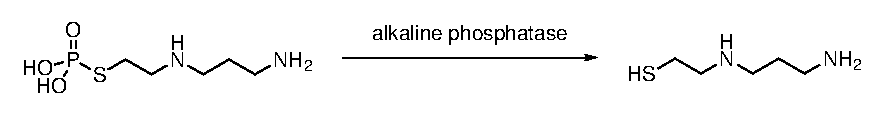
\includegraphics[scale=0.74]{Figures/amifostine.eps}
\caption{Amifostine, and its active metabolite.}
\label{fig:amifostine}
\end{figure}

Despite the clear and serious side effects of radiotherapy, there is currently only one radioprotective pharmaceutical licensed by the FDA for use as such.
Amifostine (\cref{fig:amifostine}) is administered as a prodrug, which is dephosphorylated \emph{in vivo} by alkaline phosphatase to form the free thiol which is able to scavenge radicals formed by irradiation.
Selectivity for healthy cells ultimately stems from the hypoxic nature of cancer cells, which inhibits dephosphorylation to the active compound\autocite{Kouvaris2007}.
However, due to the need for it to be present in relatively high concentration in the cytosol to effectively scavenge radicals, large doses are required, and this magnifies issues of cytotoxicity.
A more targeted approach is therefore required for effective radioprotection and a larger therapeutic window.

\subsection{Minor groove binding}
DNA is known to exist in many different structures (A-, B-, C-DNA etc.), depending on factors such as solvation and the presence of metal ions.
B-DNA, however, is by far the most prevalent in cells\autocite{Miyahara2012}.
The familiar double helix of B-DNA forms a major and a minor groove on either side of the sugar-phosphate backbone, where the nitrogenous bases are exposed.
There exists a class of small molecules which bind to this minor groove, and impart some property to the bound DNA.

The Hoechst stains, first synthesised in the early 1970s by the company \emph{Hoechst Aktiengesellschaft} as anthelmintic agents, are prototypical minor groove binders.
As can be seen in scheme \cref{fig:hoechst}, the gentle curvature of the molecule allows it to follow the DNA helix.
The benzimidazole moieties provide H-bond donors, which interact with acceptors in adenine and thymine.
At physiological pH, the molecule is positively charged, allowing further stabilisation of the DNA-Hoechst complex via electrostatic interactions with the electron rich sugar-phosphate backbone\autocite{Teng1988}.
The conjugated aromatic system imparts a strong UV absorbance at around \SI{350}{\nm}. Fluorescence in the visible spectrum is also observed, giving Hoechst compounds utility as DNA stains.

\begin{figure}
\centering
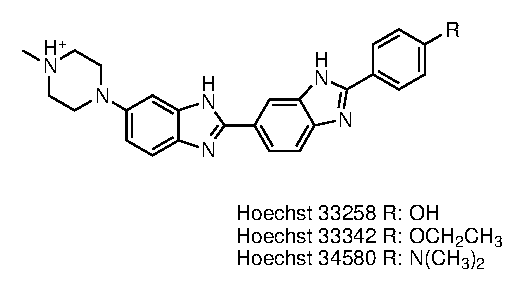
\includegraphics[scale=0.74]{Figures/hoechst.eps}
\caption{Hoechst stains, featuring the characteristic bis-benzimidaozle motif.}
\label{fig:hoechst}
\end{figure}

\subsection{Bis-benzimidazole derived radioprotectors}

In collaboration with the Peter MacCallum Cancer Centre, the White group has investigated a range of minor groove binders inspired by the Hoechst stains.
Methylproamine is a lead compound evaluated for radioprotection.
It was found to effectively protect cells from $\gamma$ and x-ray radiation, based on a clonogenic survival assay.
Pulse radiolysis studies suggested that the mechanism (for directly targeted cells) is based on direct repair of oxidative lesions, as opposed to scavenging ROS like amifostine.
When a DNA base (usually guanine) is ionised, a ``hole'' in the DNA is created.
This can be effectively transported along the length of the DNA molecule\autocite{Giese2002}.
The bound ligand (methylproamine) can then act as a reducing agent and neutralise the hole.

\begin{figure}
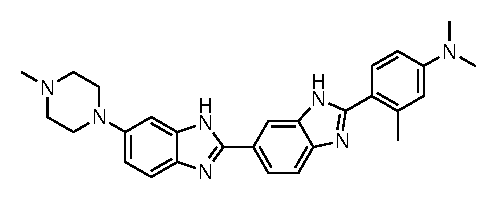
\includegraphics[scale=0.74]{Figures/methylproamine.eps}
\caption{Methylproamine, a lead compound identified for radioprotection.}
\label{fig:methylproamine}
\end{figure}

\begin{figure}
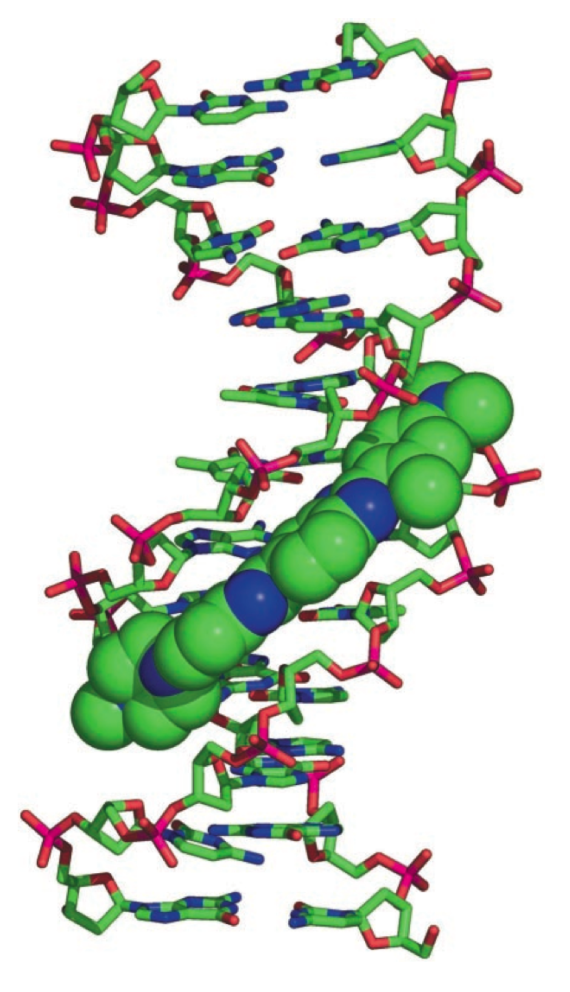
\includegraphics[width=0.3\textwidth]{Figures/mpa-dna-crystal.png}
\caption{Single crystal structure of methylproamine complexed with an AT rich DNA dodecamer.}
\label{fig:mpa-dna-crystal}
\end{figure}

\subsection{Proton-coupled electron transfer (PCET)}
The reduction mechanism of methylproamine and other bis-benzimidazole compounds is thought to be a proton-coupled electron transfer, in which an electron and proton are transferred from the ligand to the DNA in a stepwise process.
This was based on QSAR studies of a wide range of derivatives\autocite{Kakkar2005}.
It was found that the radioprotective potential was proportional to the acidity of the first benzimidazole proton.
This observation led to a new generation of radioprotectors with a 2-pyridyl group capping the first benzimidazole.
The lone pair of the pyridine nitrogen is able to donate into the $\sigma^{\star}$(N--H) antibonding orbital and weaken the bond, allowing the proton to be more easily abstracted.

Substituting the N-methyl piperazinyl group for a N-morpholino group further improved the radioprotective ability of the bis-benzimidazole.
\emph{Ab initio} modelling showed the HOMO was centred around the lone pair of the morpholine nitrogen, and x-ray crystallography indicated that, when complexed with DNA, this lone pair pointed into the minor groove in an acceptable geometry for direct electron transfer.
The lead compound M2PB \cmpd{m2pb} was therefore synthesised, and showed very promising radioprotective ability, albeit with a relatively small therapeutic window.

\begin{figure}
\replacecmpd{m2pb}
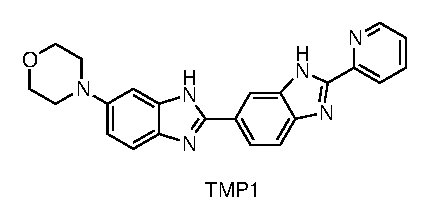
\includegraphics[scale=0.74]{Figures/m2pb.eps}
\caption{M2PB \refcmpd{m2pb}, an optimised lead compound for radioprotection.}
\label{fig:m2pb}
\end{figure}


\subsection{Chalcogens as nitrogen bioisosteres}
Heavier group VI elements such as sulfur and selenium have been observed to behave similarly to nitrogen in biological systems.
A range of drugs have been developed that display this bioisosteric behaviour\autocite{Beno2015}.
The similarity between these elements is postulated to be due to the $\sigma$-hole that heavy main group elements exhibit, and their resulting propensity for Ch-bonding.

The fundamental aspects of Ch-bonding have been throroughly discussed elsewhere in this thesis, suffice it to say that derivatives of the drug ebselen \cmpd{ebs} were identified early on as likely bioisosteres for a benzimidaozle moiety.


\subsection{Ebselen as an antioxidant}
Ebselen itself, of course, displays antioxidant properties.
These are believed to be the basis for its neuroprotective, anti-helmenthic, and anti-inflammatory behaviour.
The mechanism, however, appears to be completely different.
Ebselen behaves as a glutathione peroxidase mimic, that is to say, a catalyst that increases the rate at which glutathione reduces reactive oxygen species.

\label{sec:simplification}
For this reason, we did not constrain ourselves to 2-pyridyl analogues (as the mechanism may not involve PCET), nor did we incorporate the morpholino substituent (as the HOMO is likely to be centred on the selenium).

\section{Synthesis of analogues}
\cmpd*{m2pb}
Initial targets \cmpd{ebs-rhs-2py,ebs-ebs-2py} were identified as likely minor groove binders, based on their similarity to the bis-benzimidaozles previously studied in the group.
Due to the difficulty of functionalising the benzisoselenazolinone system and the rationailsation in \cref{sec:simplification}, we simplified our targets to exclude the morpholino group.
Among our targets, bis-benzisoselenazolinone \cmpd{ebs-ebs-2py} was particularly interesting, as it has the potential to be a completely H-bond free minor groove binder.
However, we first focussed on the synthesis of benzisoselenazolinone-benzimidaozle \cmpd{ebs-rhs-2py}, as this appeared to be the most synthetically accessible using the chemistry developed in the group.

\begin{figure}
    \centering
    \replacecmpd{m2pb}
    \replacecmpd{ebs-rhs-2py}
    \replacecmpd{ebs-ebs-2py}
    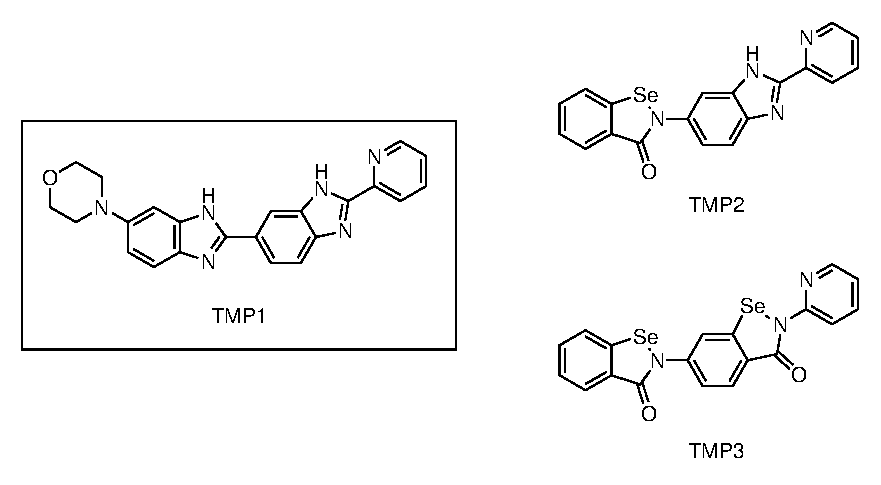
\includegraphics[scale=0.74]{Figures/targets.eps}
    \caption{Lead bis-benzimidaozle \refcmpd{m2pb} and initial target compounds \refcmpd{ebs-rhs-2py,ebs-ebs-2py}.}
    \label{fig:targets}
\end{figure}

\subsection{Preparation of benzisoselenazolinone-benzimidazole \refcmpd{ebs-rhs-2py}.}

\subsubsection{Ullman coupling}
A number of routes to this compound were envisaged, via various intermediates.
Firstly, we were inspired by the Ullman-type chemistry exploited by \citeauthor{Bhabak2010} in their selenocyclisation, and by the observation that the amidic proton in \cmpd{ebs.h} goes on to react further to furnish the tetracyclic compound \cmpd{tetracycle} (see \cref{sec:crystengcomm1})\autocite{Bhabak2010,Fellowes2019}.
We supposed that the intermediate \cmpd{ebs.h}, which can be prepared by reaction of the dichloride \cmpd{dichloride} with aqueous ammonia (\cref{sch:ebs-h-synthesis}) would be a suitable substrate for an Ullman coupling with an aryl halide.
A number of test reactions were performed using the benzisothiazolinone \cmpd{ebs.h}$\cdot$\textbf{S}, which is commercially available and inexpensive.
Typical Ullman conditions were used (high temperature, DMF solvent, high \ce{CuI} catalyst loading) to initally couple \cmpd{ebs.h}$\cdot$\textbf{S} with bromobenzene to afford \cmpd{ebs}$\cdot$\textbf{S} in moderate yield (\cref{sch:ebs-thio-ph-synthesis}).
We were also able to prepare ebselen \cmpd{ebs} via this route in similar yield.
Optimisation of the reaction was considered to be outside the scope of this work, so we proceeded with the synthesis of the bromo-benzimidazole coupling partner \cmpd{rhs-bromo-2py}.

\begin{scheme}
    \replacecmpd{dichloride}
    \replacecmpd{ebs.h}
    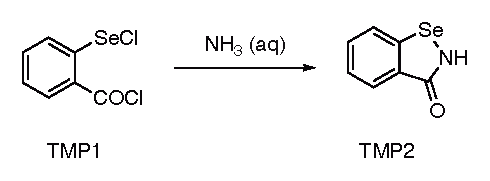
\includegraphics[scale=0.74]{Figures/ebs-h-synthesis.eps}
    \caption{Synthesis of \refcmpd{ebs.h}.}
    \label{sch:ebs-h-synthesis}
\end{scheme}

\begin{scheme}
    \replacecmpd{ebs.h}
    \replacecmpd{ebs}
    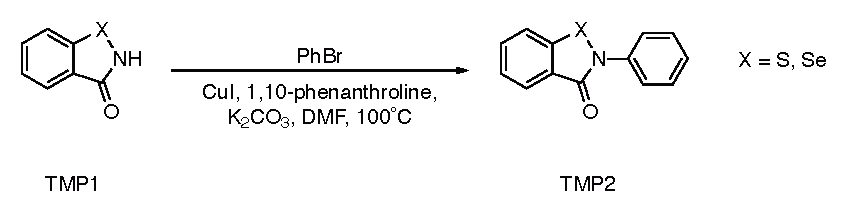
\includegraphics[scale=0.74]{Figures/ebs-thio-ph-synthesis.eps}
    \caption{Synthesis of \refcmpd{ebs}.}
    \label{sch:ebs-thio-ph-synthesis}
\end{scheme}
\label{sec:carboximidate}

4-bromo-2-nitroaniline was reduced to the diamine \cmpd{bromodiamine} using tin (II) chloride, then reacted with 2-pyridyl carboximidate hydrochloride \cmpd{2py-carboximidate} (prepared from 2-pyridyl carbonitrile) to afford the benzimidazole \cmpd{rhs-bromo-2py} in excellent yield.
Unfortunately this gave no detectable product in the coupling reaction.
We suspected that the benzimidazole proton may be competing with the amidic proton in the benzisothiazolinone ring, as it is substantially more acidic (pKa 16.4 vs $>20$), so we protected it using \emph{p}-methoxy benzyl chloride to give \cmpd[sub-counter-format=pg]{rhs-bromo-2py.pmb} (\cref{sch:rhs-protection}).
This afforded two distinct isomers from the two freely interconverting tautomers of \cmpd{rhs-bromo-2py}.
Although these were resolved by chromatography for subsequent reactions, this was likely not necessary, as deprotection would afford both tautomers.
Both isomers are therefore treated as a single compound here.

\begin{scheme}
    \replacecmpd{2py-carboximidate}
    \replacecmpd{bromodiamine}
    \replacecmpd{rhs-bromo-2py}
    \replacecmpd{rhs-bromo-2py.pmb}
    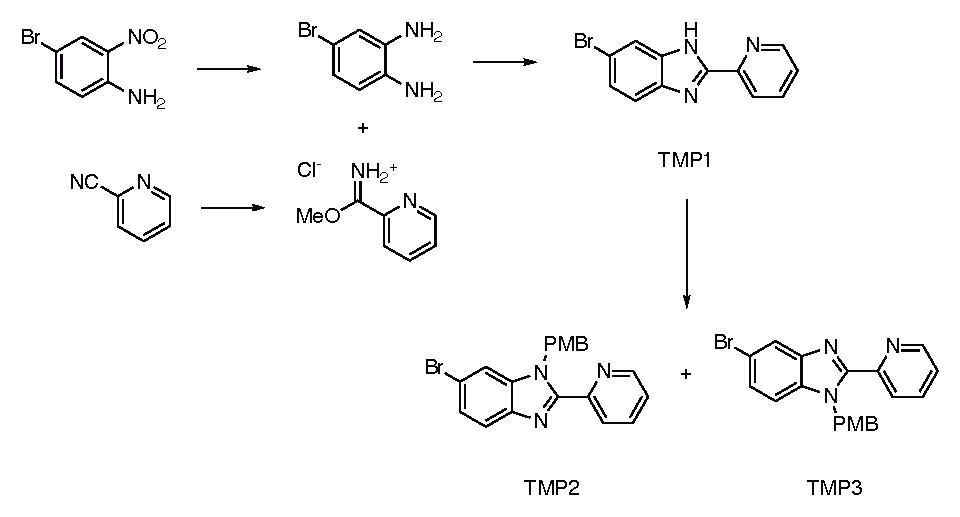
\includegraphics[scale=0.74]{Figures/rhs-protection.eps}
    \caption{Synthesis of \refcmpd{rhs-bromo-2py} and protection to form \refcmpd{rhs-bromo-2py.pmb}. a) \ce{SnCl2.2H2O}, ethanol, reflux; b) \ce{NaOMe}, methanol, acetic acid; c) Methanol, reflux; d) \ce{NaH}, PMBCl, DMF, 0\degree C $\rightarrow$ r.t.}
    \label{sch:rhs-protection}
\end{scheme}

The PMB-protected benzimidazoles also gave no detectable coupling product, so we turned our attention to the catalyst/ligand system.
Ullman couplings require a bidentate nitrogen-based ligand to coordinate the copper (I) species.
We used dimethylethylenediamine (DMEDA), although salicylates, 1,10-phenanthroline, 2,2\textprime-bipyridyl, tetramethylethylenediamine, and proline have also been used sucessfully in similar reactions.\autocite{Klapars2002,Altman2007,Sherborne2017}
The 2-(2-pyridyl)benzimidazole, even protected, resembles these ligands, and could reasonably be anticipated to coordinate the copper in competition with the ligand.
Although this does not necessarily preclude the coupling reaction, it does remove our ability to modify the coordination environment of the copper, to which the Ullman reaction is very sensitive.
We attempted a ligand-free reaction to no avail, and thus concluded that the coordination environment of the copper is inappropriate for the reaction, and we would have to use another substrate.

We therefore prepared the phenyl derivative \cmpd{rhs-bromo-ph} via a metabisulfite coupling with benzaldehyde, and protected it similarly to give both isomers of \cmpd[sub-counter-format=pg]{rhs-bromo-ph.pmb}.
This gave the desired coupling product \cmpd[sub-counter-format=pg]{ebs-rhs-ph.pmb}$\cdot$\textbf{S} as a mixture of isomers, from one of which we obtained a single crystal structure (\cref{sch:ebs-thio-rhs-synthesis} and \cref{fig:ebs-thio-rhs-pmb-xray}).
We were also able to prepare the benzisoselenazolinone derivative \cmpd[sub-counter-format=pg]{ebs-rhs-ph.pmb} as a pair of isomers.
Unfortunately, all efforts to deprotect the benzimidazole nitrogen failed.
A number of other protecting groups were trialled, including trityl, triphenylsilyl, \emph{t}-butyl and ethyl carbamates, however all either failed to give any protected product, or were too labile to survive the Ullman reaction conditions.
We therefore abandoned this synthetic route.

\begin{scheme}
    \replacecmpd{ebs.h}
    \replacecmpd{rhs-bromo-ph.pmb}
    \replacecmpd{ebs-rhs-ph.pmb}
    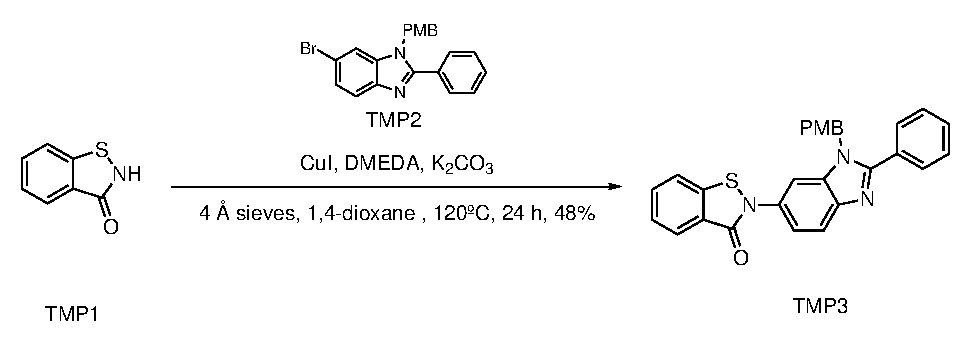
\includegraphics[scale=0.74]{Figures/ebs-thio-rhs-synthesis.eps}
    \caption{Synthesis of \refcmpd{ebs-rhs-ph.pmb}.}
    \label{sch:ebs-thio-rhs-synthesis}
\end{scheme}

\begin{figure}
    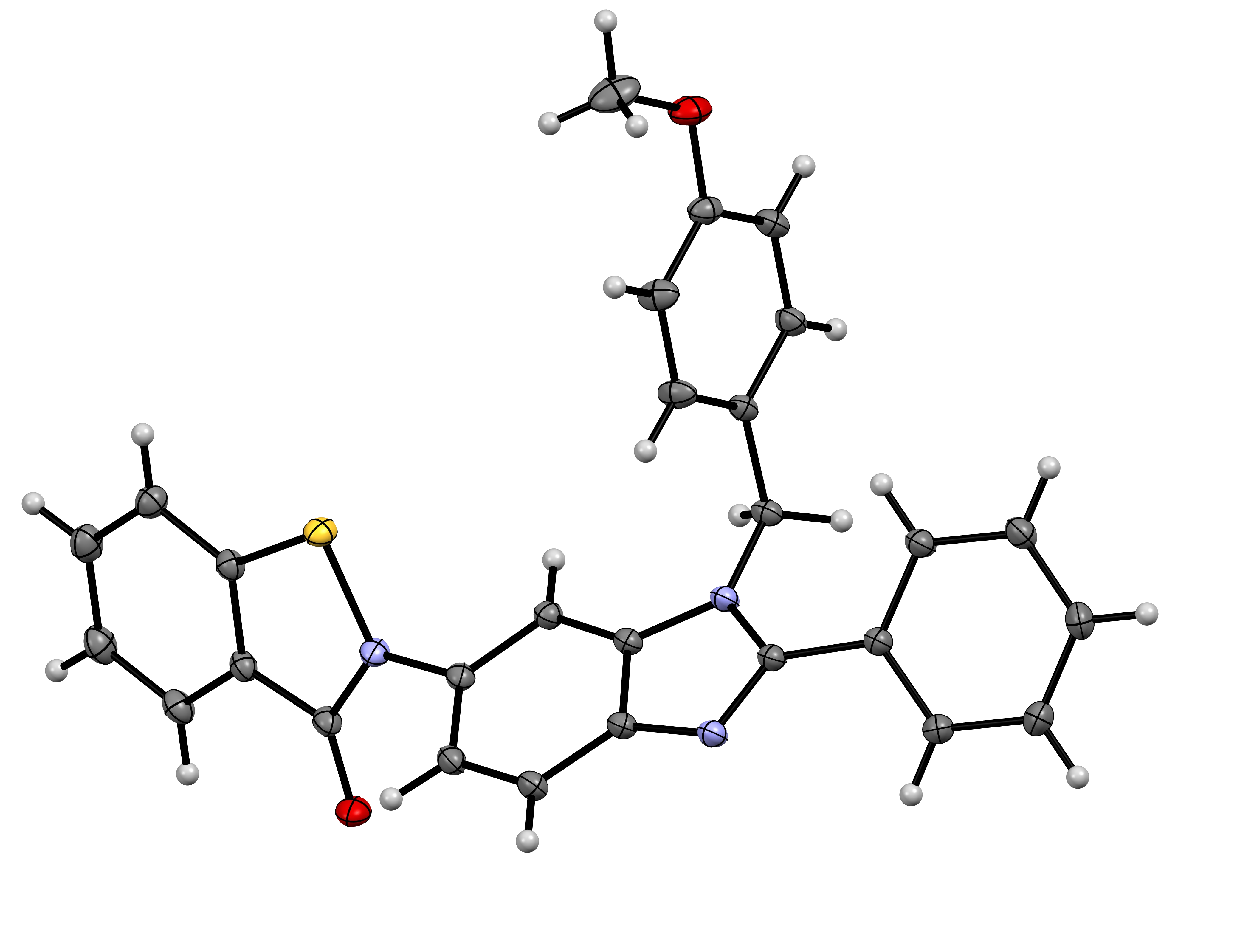
\includegraphics[width = 0.8\linewidth]{Figures/ebs-thio-rhs-pmb-xray.pdf}
    \caption{X-ray crystal structure of one isomer of \refcmpd{ebs-rhs-ph.pmb}$\cdot$\textbf{S}.}
    \label{fig:ebs-thio-rhs-pmb-xray}
\end{figure}

\subsubsection{Benzisoselenazolinone-first route}

\begin{scheme}
    \replacecmpd{diselenide}
    \replacecmpd{dichloride}
    \replacecmpd{ebs-nitroaniline}
    \replacecmpd{ebs-nitroamide-2py}
    \replacecmpd{ebs-rhs-2py}
    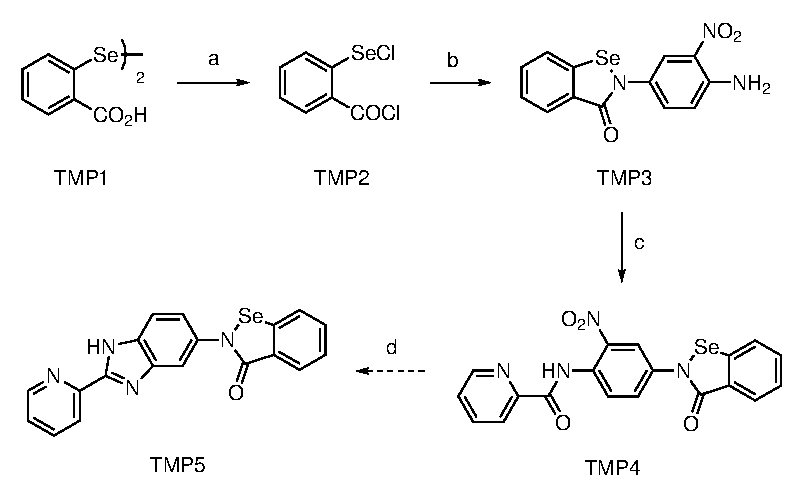
\includegraphics[scale=0.74]{Figures/ebs-synthesis3.eps}
    \caption[Proposed synthesis of \refcmpd{ebs-rhs-2py}]{Proposed synthesis of \refcmpd{ebs-rhs-2py}. a) \ce{SOCl2}, b) 2-nitro-1,4-benzenediamine, \ce{Et3N}, THF, c) Picolinic acid, TCBC/DMAP, \ce{Et3N}, d) [H], \ce{H+}.}
    \label{sch:ebs-rhs-synthesis-1}
\end{scheme}

A revised route to this molecule is shown in \cref{sch:ebs-rhs-synthesis-1}, which involved first synthesising the benzisoselenazolinone moiety, then constucting the benzimidazole in a condensation and reductive dehydrocyclisation.
The results of this, specifically the interesting crystal packing of the late stage intermediate \cmpd{ebs-nitroamide-2py} spurred the investigation detailed in \cref{sec:thermal-conversion}.
As this pathway did not involve copper catalysis, we reintroduced the 2-pyridyl group on the benzimidazole.
However, this route was not able to furnish the desired product, as the benzisoselenazolinone moiety did not tolerate the reduction conditions trialled.
Among the conditions trialled were:
\begin{itemize}
    \item palladium catalysed hydrogenation, from which we only recovered starting material presumably due to the catalyst being poisoned by the divalent selenium,
    \item tin (II) chloride/HCl reduction, which afforded a diselenide \cmpd{ebs-rhs-2py-diselenide} (\cref{fig:diselenide-benzimidazole-2py-xray}),
    \item dithionite reduction, which afforded a complex mixture of products.
    \label{sec:reduction}
\end{itemize}

\begin{figure}
    \centering
    \replacecmpd{ebs-rhs-2py-diselenide}
    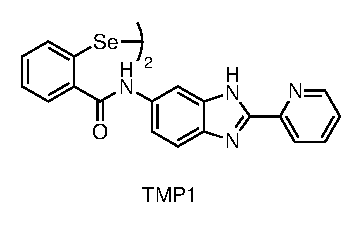
\includegraphics[scale=0.74]{Figures/ebs-rhs-diselenide.eps}

    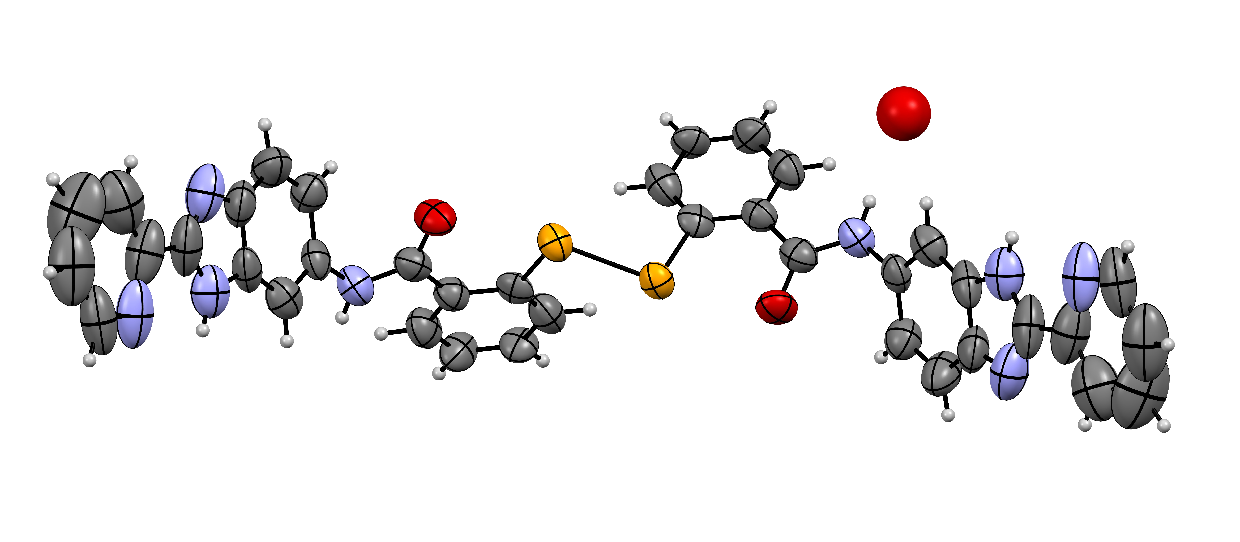
\includegraphics[width=0.8\linewidth]{Figures/diselenide-benzimidazole-2py-xray.pdf}
    \caption[X-ray crystal structure of \refcmpd{ebs-rhs-2py-diselenide}.]{X-ray crystal structure of \refcmpd{ebs-rhs-2py-diselenide} with a disordered water molecule.}
    \label{fig:diselenide-benzimidazole-2py-xray}
\end{figure}

\subsubsection{Benzisoselenazoline-last route}

\begin{scheme}
    \replacecmpd{rhs-nitro-amide}
    \replacecmpd{rhs-nitro}
    \replacecmpd{rhs-amine}
    \replacecmpd{ebs-rhs-ph}
    \caption{Synthesis of benzisoselenazolinone-benzimidazole Hoechst analogue \refcmpd{ebs-rhs-ph}.}
    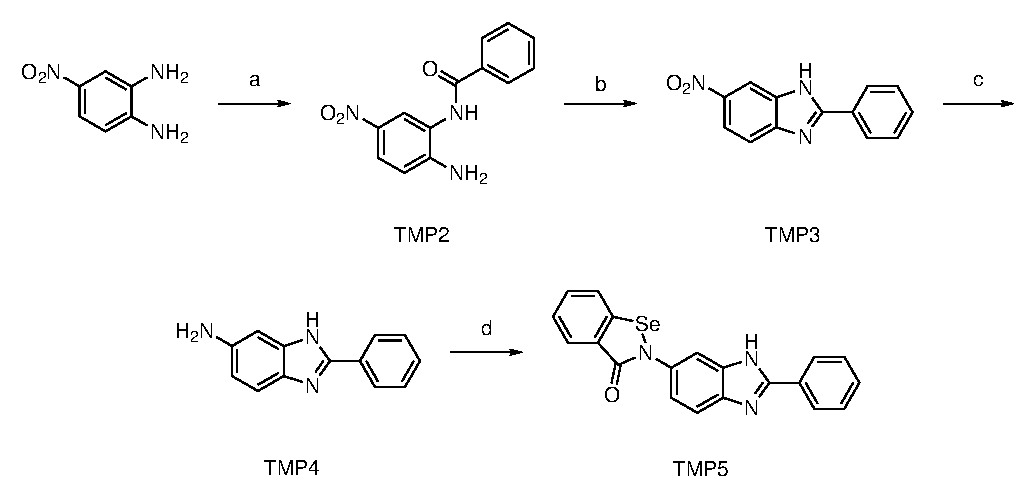
\includegraphics[scale=0.74]{Figures/ebs-rhs-synthesis.eps}
    \label{sch:ebs-rhs-synthesis-2}
\end{scheme}

We therefore devised another scheme in which the benzisoselenazolinone ring is formed last, as the delicate nature of this group appeared to be hindering our efforts (\cref{sch:ebs-rhs-synthesis-2}).
This initially involved formation of an amide \cmpd{rhs-nitro-amide} by treating 3,4-diamino-1-nitrobenzene with an acid chloride.
It was found that the acid chloride of picolinic acid (which would ultimately afford the 2-(2-pyridyl) benzimidazole) was not stable, decomposing almost as soon as it was formed.
We investigated using the carboximidate as in \cref{sec:carboximidate}, however the nitro group on the diamine proved to be too deactivating; the aniline nitrogens were not sufficiently nucleophilic to react with the carboximidate.
Rather than investigate other pathways to this compound (such as the use of coupling agents), we again decided to simplify the system to a phenyl ring (to ultimately give \cmpd{ebs-rhs-ph}).
We therefore formed \cmpd{rhs-nitro-amide} using benzoyl chloride in excellent yield, which underwent a dehydrocyclisation in the presence of the strong Lewis acid \ce{BF3\cdot OEt2} to form \cmpd{rhs-nitro}.
Tin (II) chloride reduction of the nitroarene \cmpd{rhs-nitro} afforded the aniline \cmpd{rhs-amine} as the hexachlorostannate salt.
This was coupled to the bis-electrophile \cmpd{dichloride} to afford the desired benzisoselenazolinone-benzimidaozle \cmpd{ebs-rhs-ph}, which formed single crystals suitable for x-ray diffraction by slow evaporation from DMSO (\cref{fig:ebs-rhs-xray}).

\begin{figure}[ht]
    \centering
    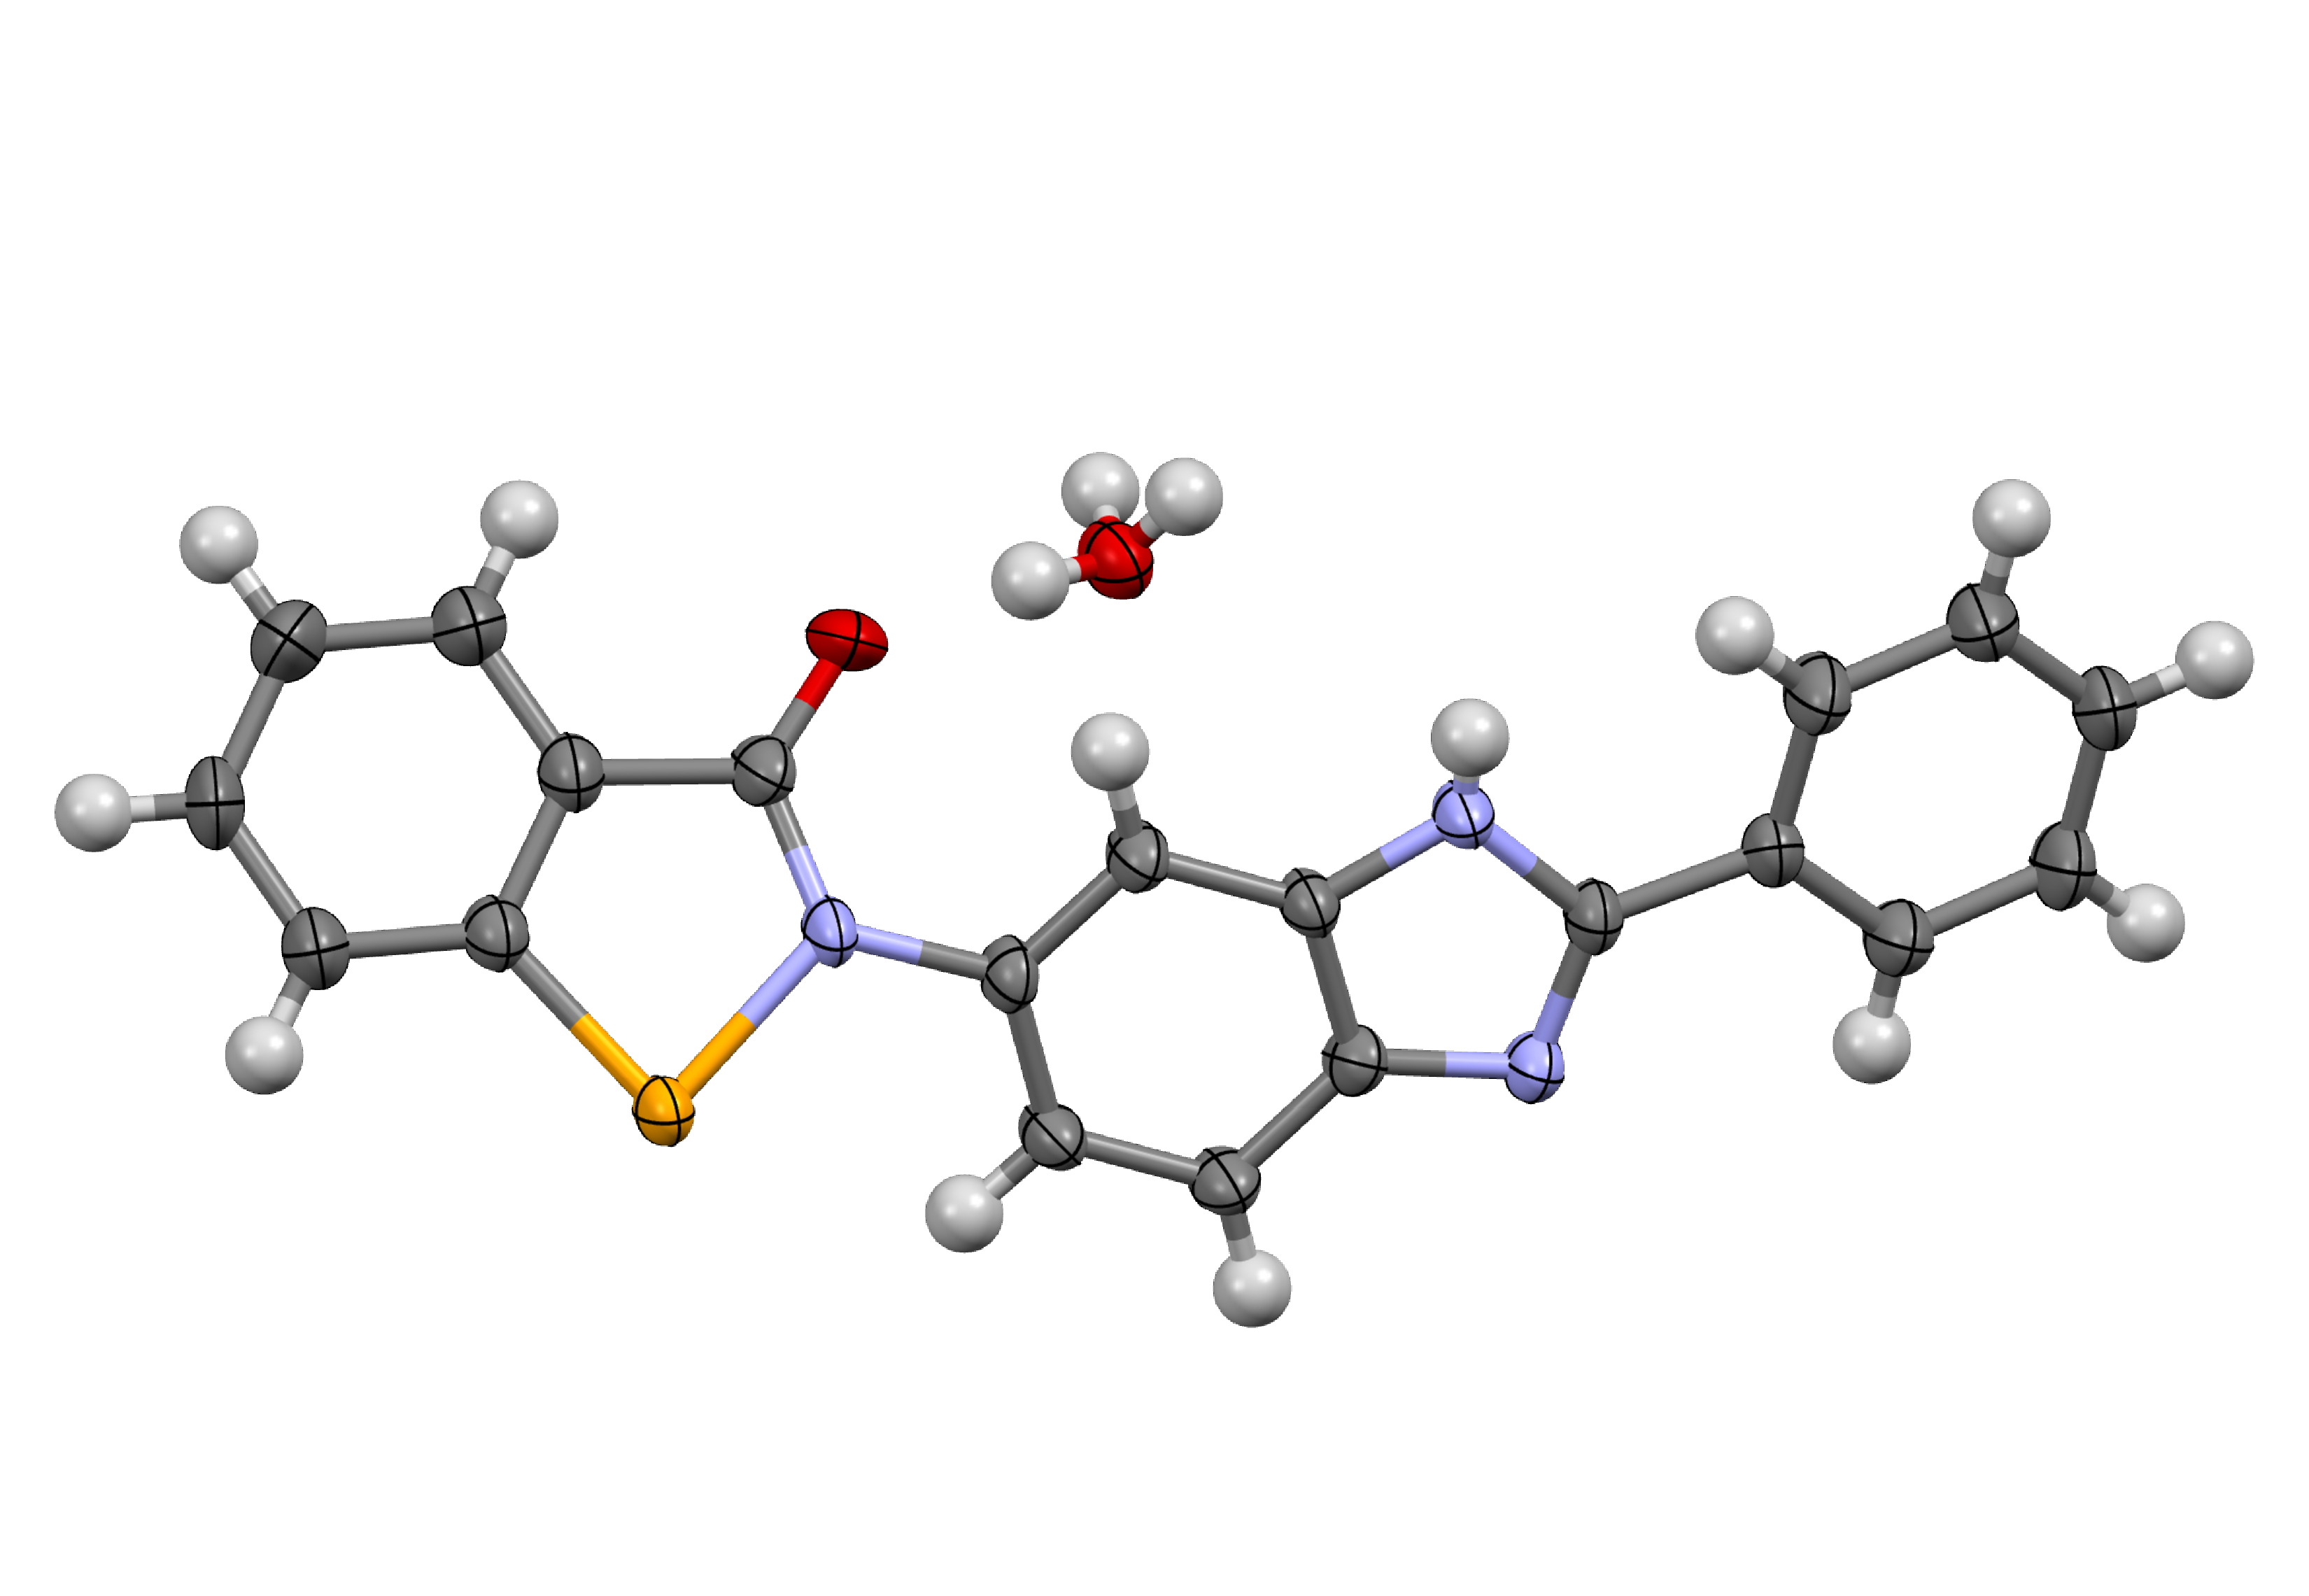
\includegraphics[width=0.8\linewidth]{Figures/ebs-rhs-xray.pdf}
    \caption[X-ray crystal structure of \refcmpd{ebs-rhs-ph}.]{X-ray crystal structure of \refcmpd{ebs-rhs-ph}. The water is disordered over 3 sites, with each proton having an occupancy of 2/3.}
    \label{fig:ebs-rhs-xray}
\end{figure}

\begin{comment}
\subsection{Preparation of bis-benzisoselenazolinone \refcmpd{ebs-ebs-2py}.}

The fused ring system of the benzisoselenazolinone proved to be difficult to functionalise.
The only reproducible method that we trialled was the selenocyclisation of \citeauthor{Bhabak2010}, using functionalised \emph{o}-halo benzamides as the substrate.\autocite{Bhabak2010}
This method was signifcantly simpler than preparing functionalised diselenides for subsequent chlorination to give analogs of the dichloride \cmpd{dichloride}, due to the solubility and safety issues encountered in the diazotisation reaction.

\begin{scheme}
    \replacecmpd{2cl-4no2-amide}
    \replacecmpd{ebs-3no2}
    \replacecmpd{ebs-3nh2}
    \replacecmpd{dichloride}
    \replacecmpd{ebs-ebs-2py}
    \caption{Synthesis of bis-benzisoselenazolinone Hoechst analogue \refcmpd{ebs-ebs-2py}.}
    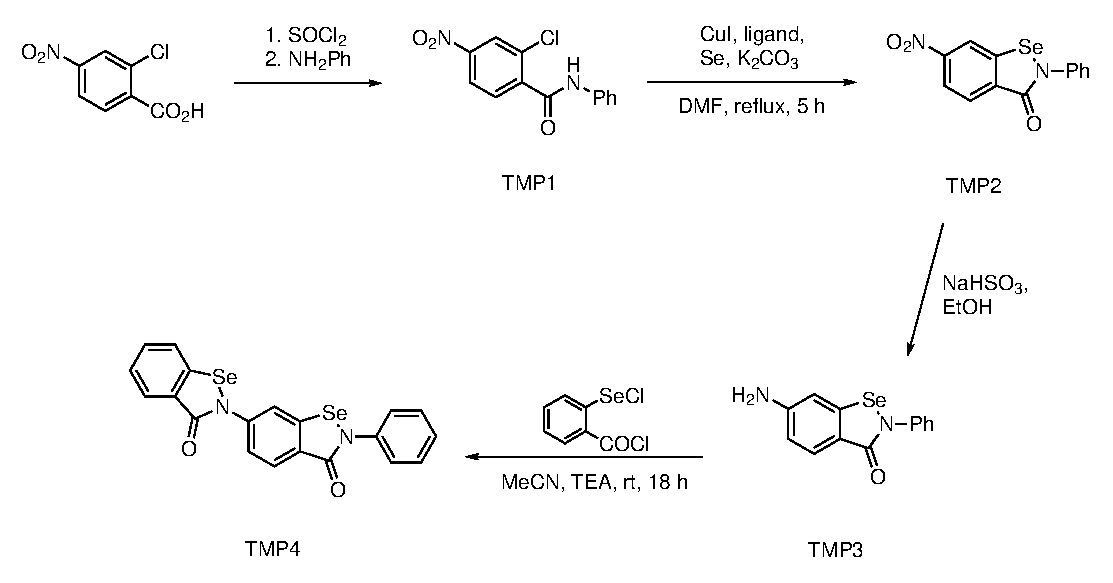
\includegraphics[scale=0.74]{Figures/ebs-ebs-synthesis.eps}
    \label{sch:ebs-ebs-synthesis}
\end{scheme}

To this end, we first targeted the amino-benzisoselenazolinone \cmpd{ebs-3nh2}, envisaging that we could then couple it to the dichloride \cmpd{dichloride} as we had done in the previous section.
Starting from 2-chloro-4-nitrobenzoic acid, we prepared the amide \cmpd{2cl-4no2-amide} from the corresponding acid chloride and aniline in quantitative yield.
This was then subjected to the selenocyclisation reaction, affording the functionalised benzisoselenazolinone \cmpd{ebs-3no2} in modest yield.
The details of this synthesis are shown in \cref{sch:ebs-ebs-synthesis}.
Reduction of the nitro group proved challenging, as the same issues were encountered as in \cref{sec:reduction}.
We therefore required a method to avoid any reduction of the nitro group in the presence of the benzisoselenazolinone.

Instead, the nitro group of \cmpd{2cl-4no2-amide} was reduced to the aniline \cmpd{2cl-4nh2-amide} using tin (II) chloride dihydrate, which was protected as the phthalimide \cmpd{2cl-4nh2-phthal-amide} to prevent side reactions in the subsequent selenocyclisation.

\begin{scheme}
    \replacecmpd{2cl-4no2-amide}
    \replacecmpd{2cl-4nh2-amide}
    \replacecmpd{2cl-4nh2-phthal-amide}
    \replacecmpd{ebs-3nh2-phthal}
    \replacecmpd{ebs-3nh2}
    \replacecmpd{dichloride}
    \replacecmpd{ebs-ebs-2py}
    \caption{Revised synthesis of bis-benzisoselenazolinone Hoechst analogue \refcmpd{ebs-ebs-2py}.}
    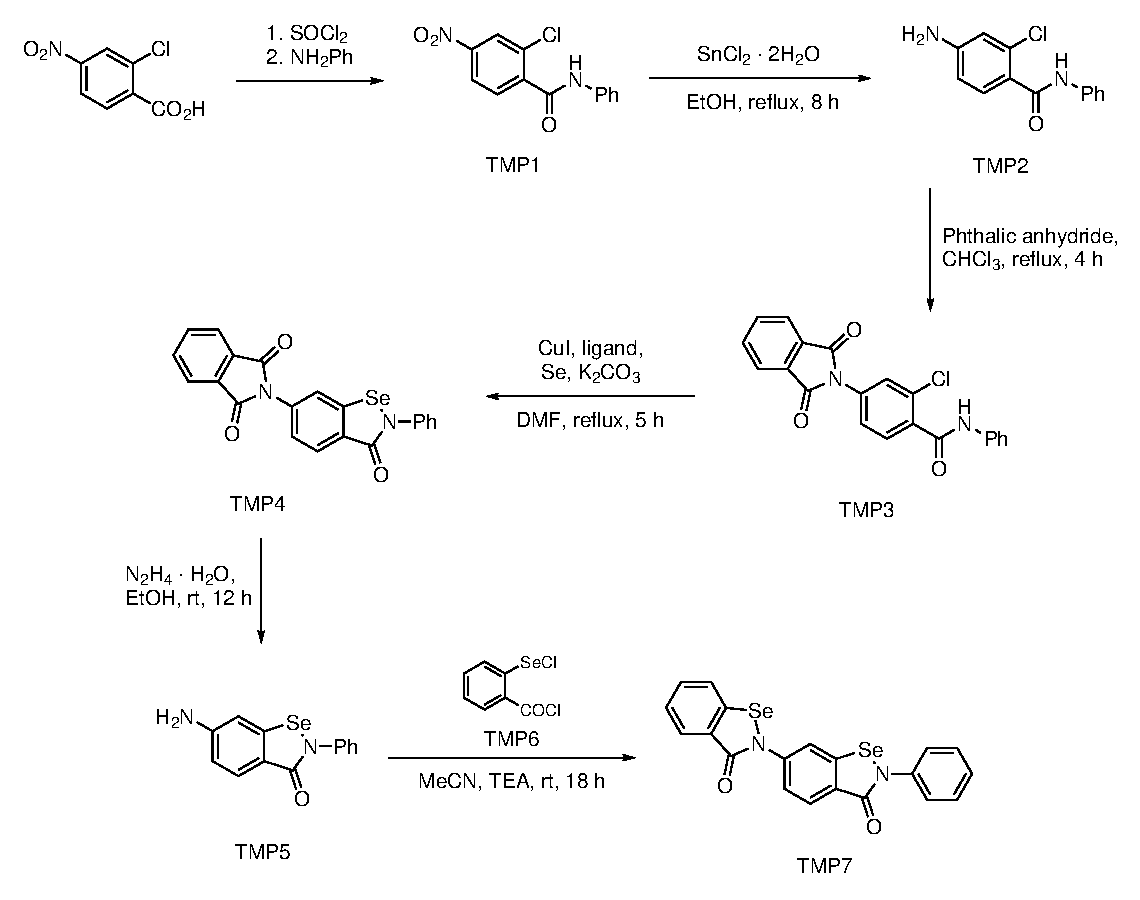
\includegraphics[scale=0.74]{Figures/ebs-ebs-synthesis-2.eps}
    \label{sch:ebs-ebs-synthesis-2}
\end{scheme}
\end{comment}

\section{Cell imaging}

BOH

Owyong/Alex do

The Hoechst compounds (upon which the group's radioprotectors are based) were originally designed and used as stains, due to their high affinity for DNA and their favourable photophysical properties.
The free compounds absorb strongly at around 350~nm (for Hoechst 33258), which is modulated slightly upon binding to the minor groove of DNA (see \cref{sec:absorbance} for a more detailed discussion).
Furthermore, the fluorescence quantum yield is extremely high, with fluorescence visible under ambient light at around 450~nm (\cref{fig:hoechst-fluorescence}).

\begin{figure}
    \centering
    OWYONG TO FIND BETTER PICTURE???
    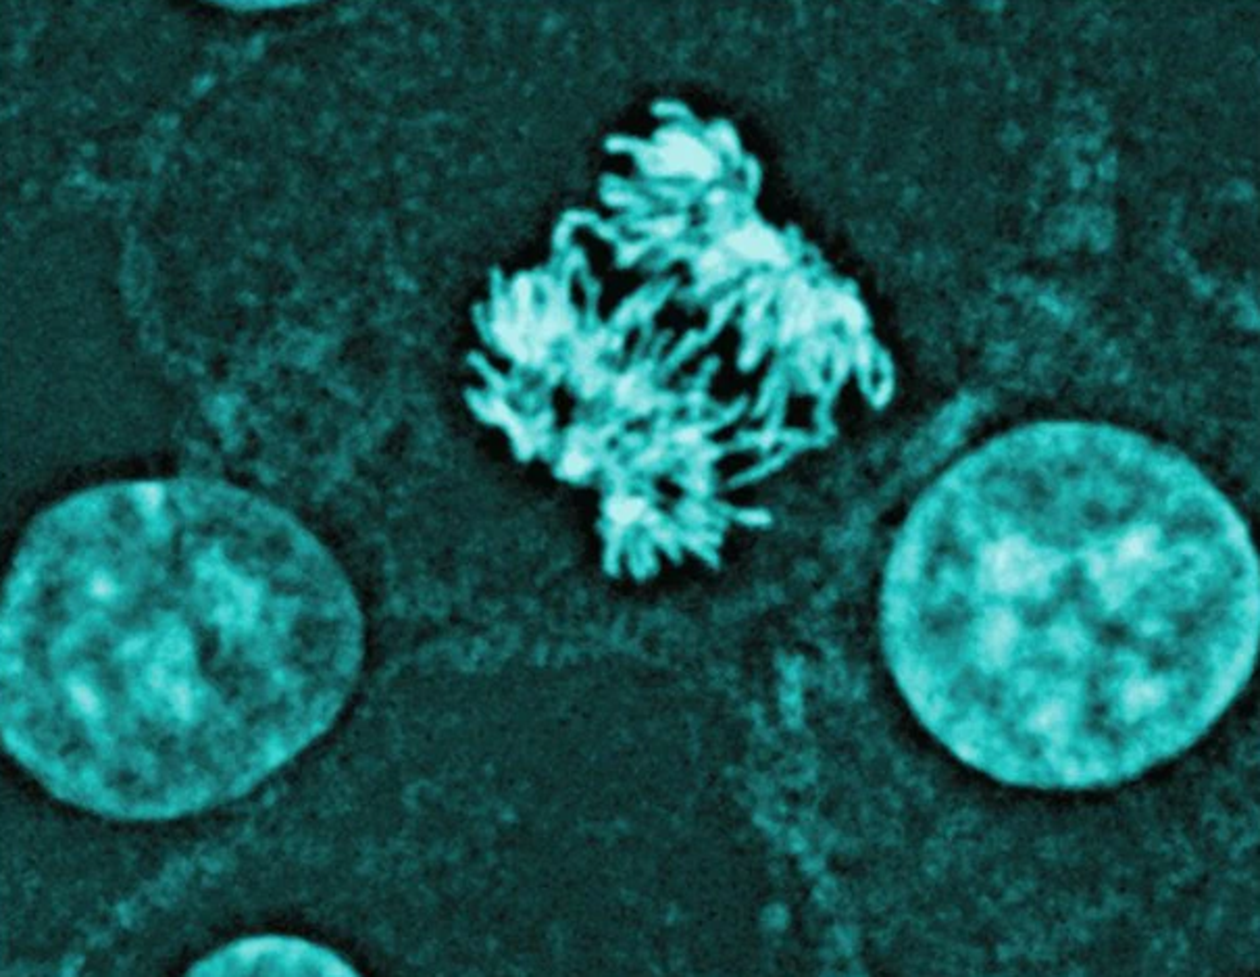
\includegraphics[width=0.6\linewidth]{Figures/hoechst-cells.pdf}
    \caption{Cells stained with Hoechst 33342 showing nuclear localisation. The central cell is undergoing mitosis.}
    \label{fig:hoechst-cells}
\end{figure}

\begin{figure}
    \centering
    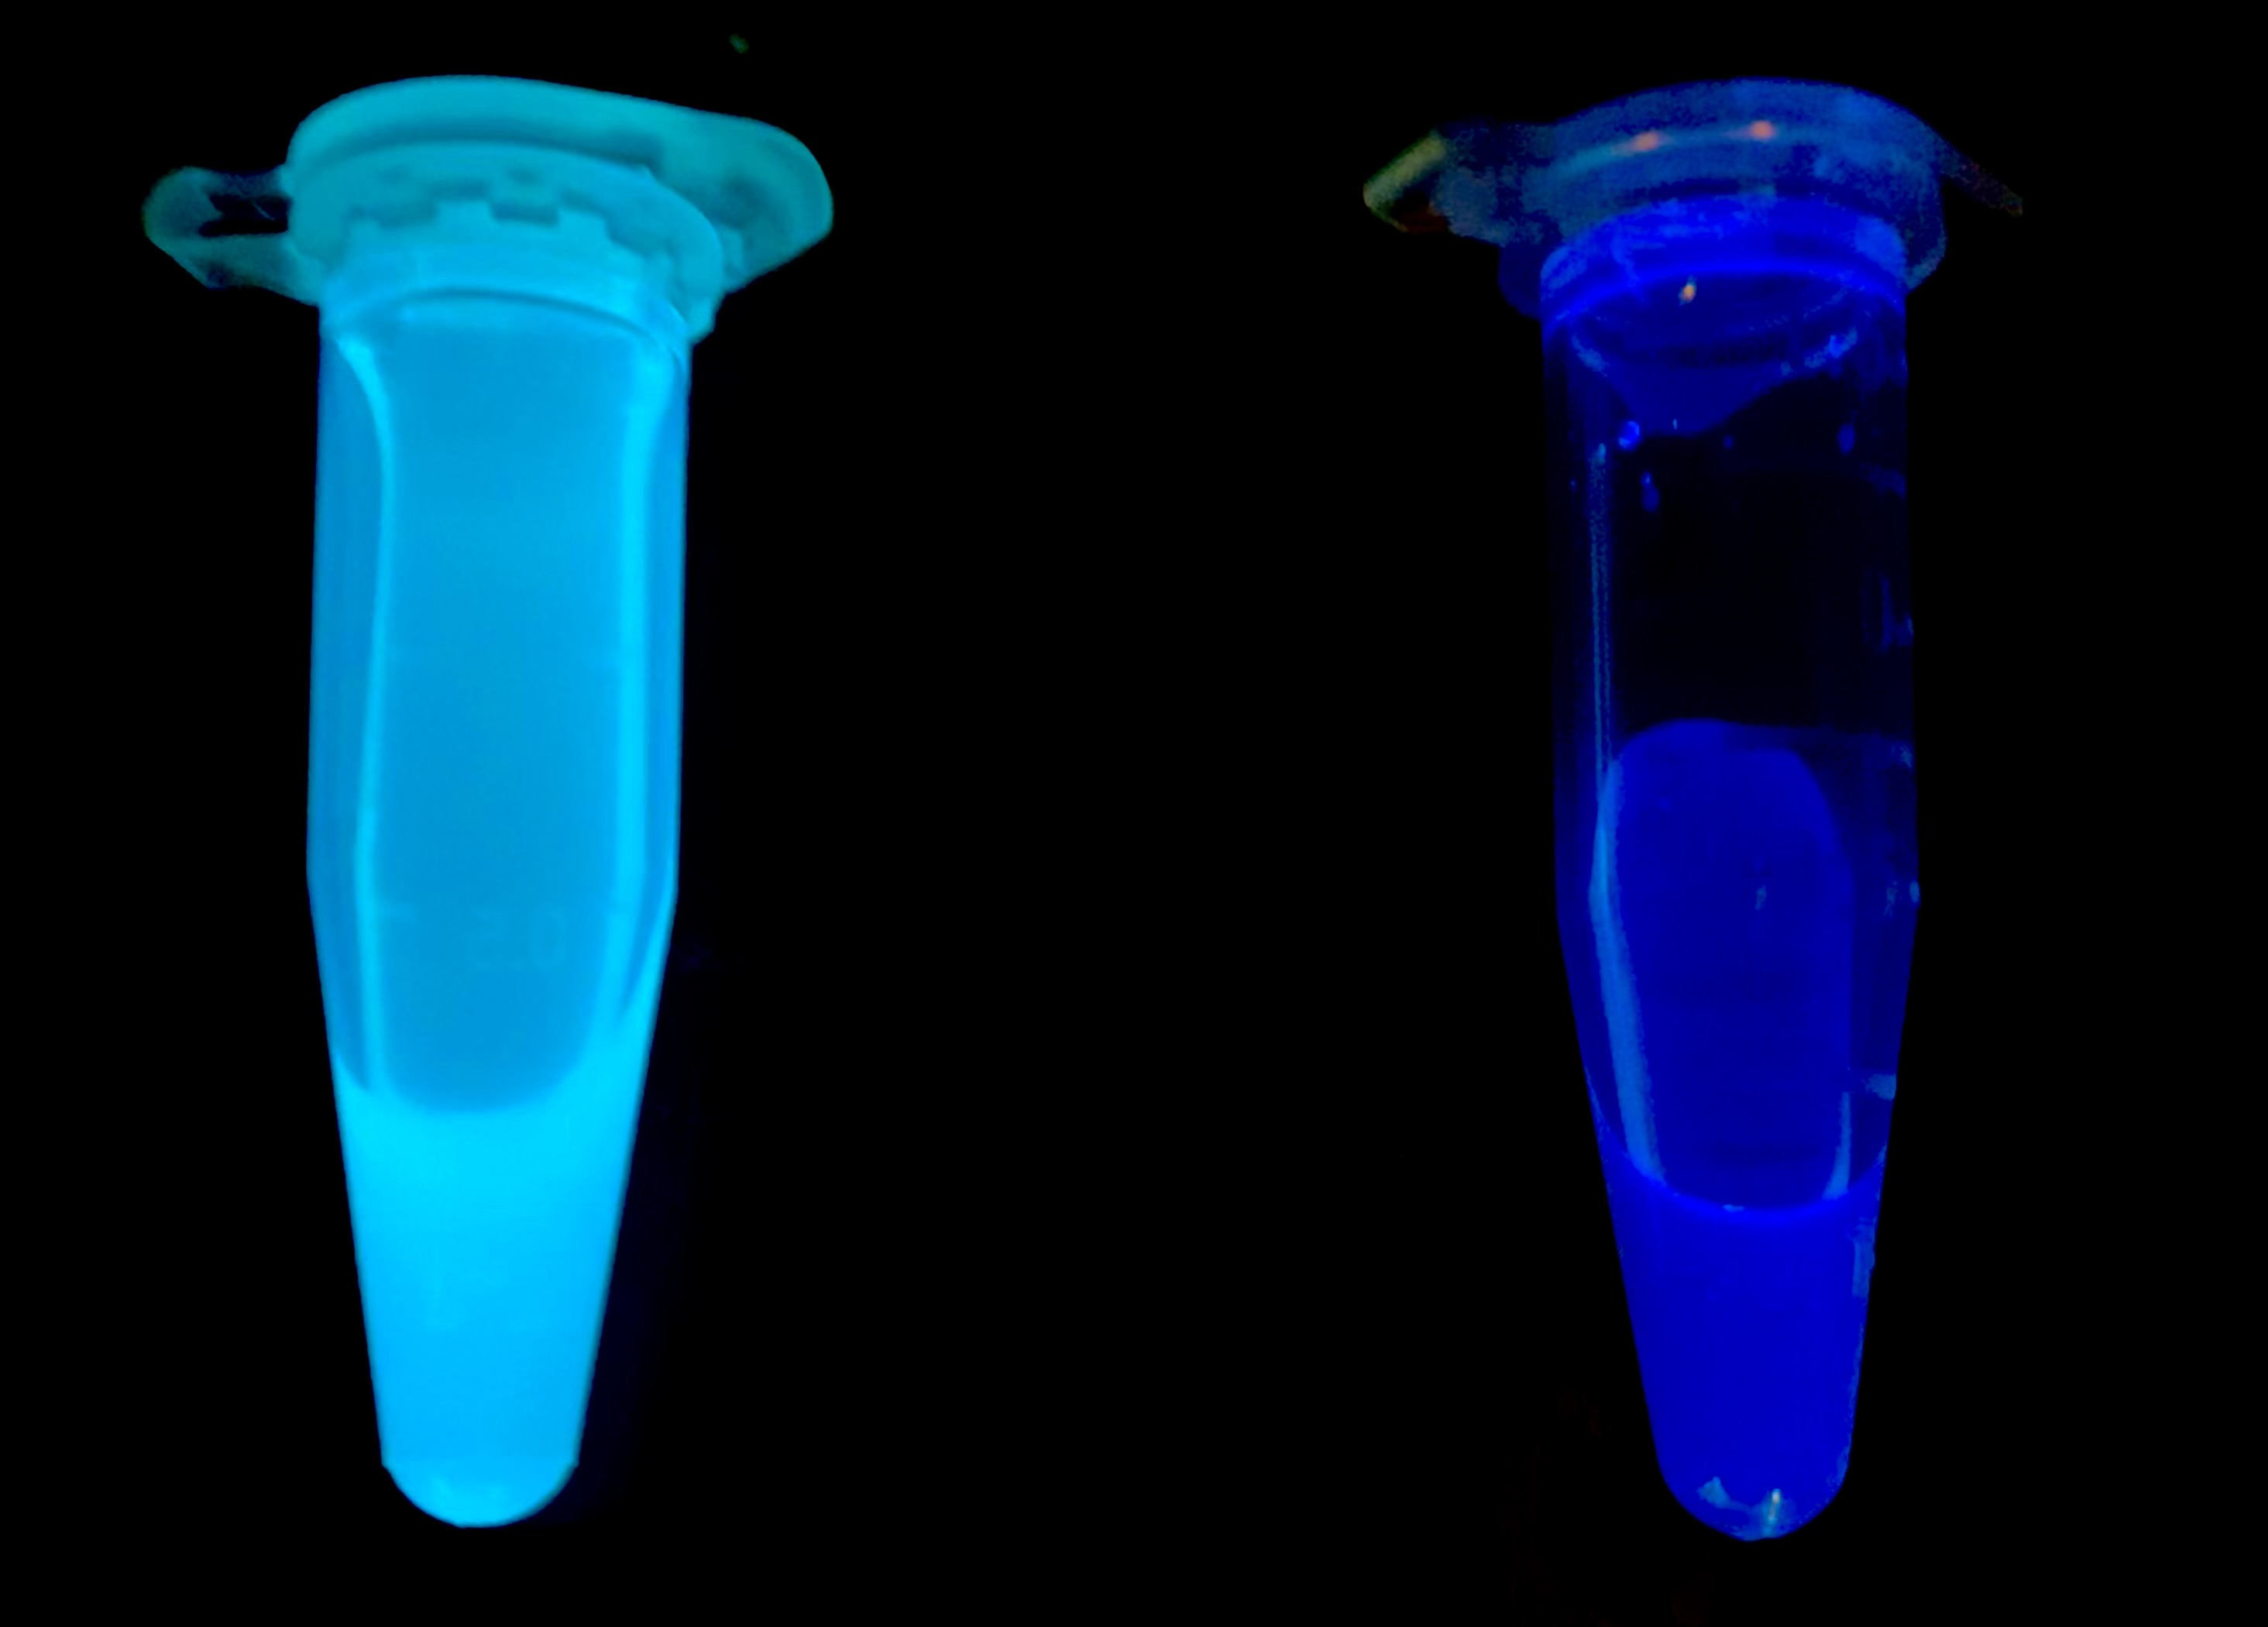
\includegraphics[width=0.6\linewidth]{Figures/hoechst-fluoresence.jpg}
    \caption{Visible fluoresence of methylproamine (left) and benzisoselenazolinone \refcmpd{ebs-rhs-ph}.}
    \label{fig:hoechst-fluorescence}
\end{figure}

Fortunately, the benzisoselenazolinone-benzimidazole \cmpd{ebs-rhs-ph} shows similar photophysical properties.
Absorption and fluorescence spectra are presented in \cref{fig:ebs-rhs-spectra}.
The absorption peak is blueshifted slightly to around 315~nm, and the emission is slightly redder at around 460~nm,
The fluorescence is noticably quenched in chloroform and, to a lesser extent, DMSO.
The reason for this is not clear???.

\begin{figure} 
    \centering
    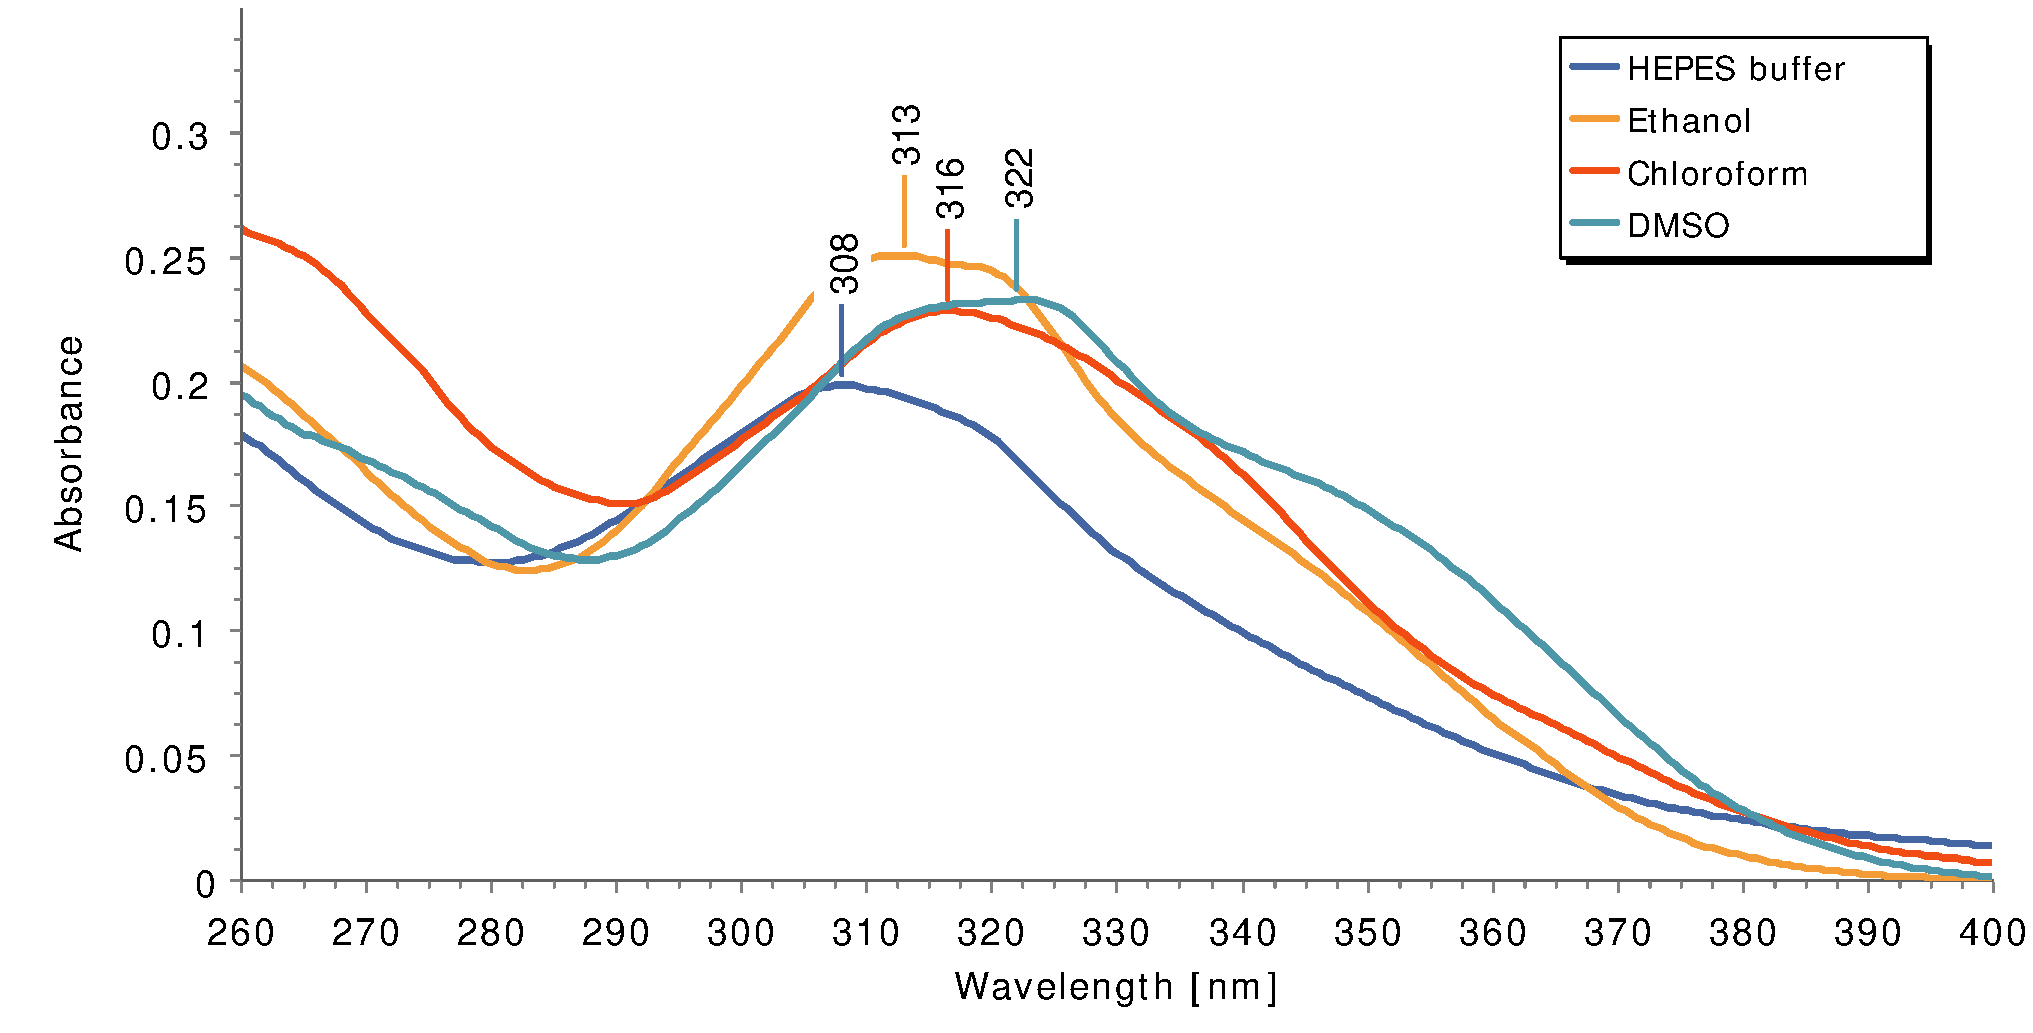
\includegraphics[width=0.95\linewidth]{Figures/ebs-rhs-abs.pdf}

    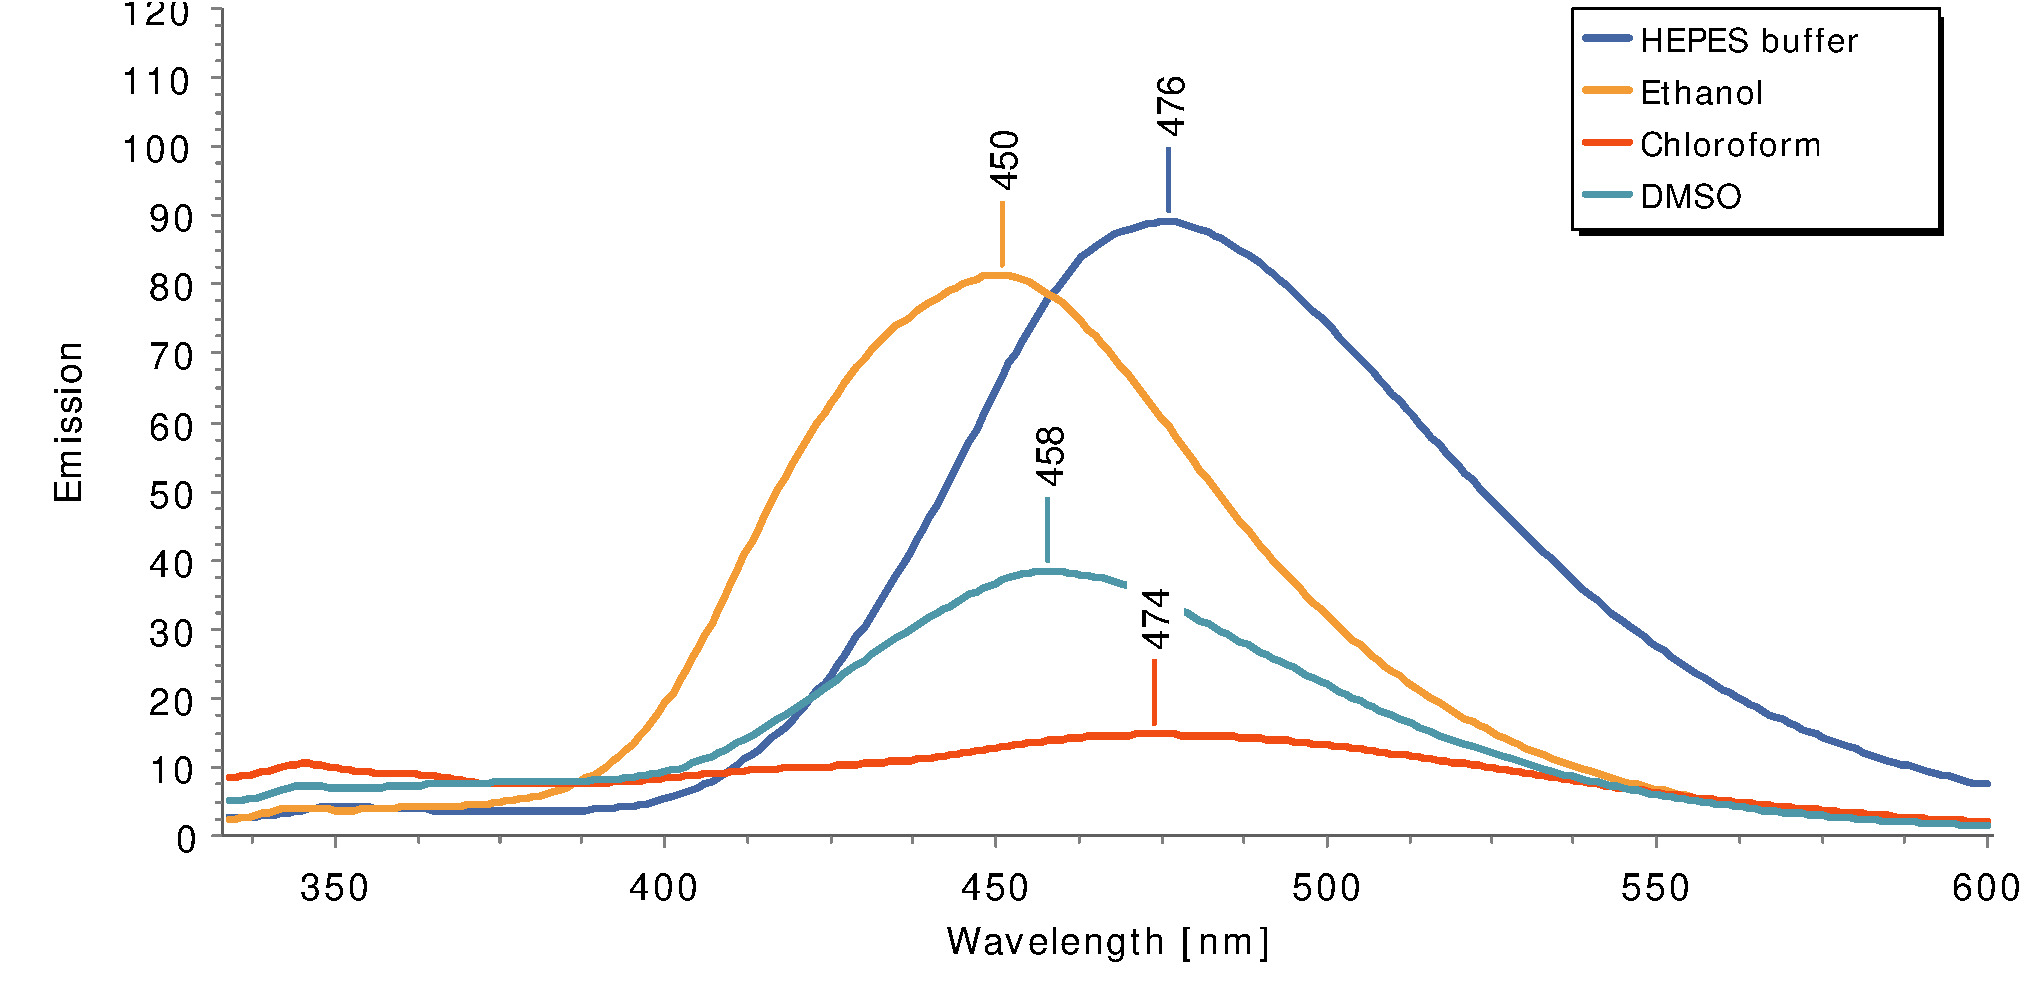
\includegraphics[width=0.95\linewidth]{Figures/ebs-rhs-fl.pdf}
    \caption{Absorbance and emission spectra of \refcmpd{ebs-rhs-ph} in various solvents.}
    \label{fig:ebs-rhs-spectra}
\end{figure}

To demonstrate that the benzisoselenazolinone \cmpd{ebs-rhs-ph} may also be used as a stain, we DID SOME STUFF???



\section{DNA binding studies}
Previous studies of Hoechst derivatives have shown that radioprotective ability is strongly correlated with a high affinity for the minor groove of DNA.
Although it is conceivable that ROS may be reduced in the cytoplasm by radioprotector molecules, this does not appear to be the major method of radioprotection for these compounds.

\subsection{Background}
DNA binding studies are a relatively fast and simple preliminary method to determine radioprotective potential, which is invalulable for providing rapid feedback into the molecular design and synthesis steps.
Without a fast screening assay, radioprotection would have to be assessed directly using either pulse radiolysis or clonogenic survival assays, both of which require specialised facilities with an associated cost.

\subsubsection{UV-Vis titration}
\label{sec:absorbance}
Two major techniques have been used in this project to determine DNA binding affinity.
The first is a UV-vis titration of a DNA oligomer into a solution of the ligand.
Briefly, this works by measuring the degree of conjugation between the two benzimidazole (or benzimidazole-like) systems.
Free bis-benzimidazoles have a significant torsion about the central bond, partially due to the push-pull character of these compounds.
This leads to relatively poor orbital overlap and conjugation between the benzimidazoles, and an associated blue shift in the absorbance spectrum as compared to a completely planar molecule.
As the bis-benzimidazole binds to the minor groove of a DNA molecule, a more planar geometry is imposed, so the orbital overlap is improved and the absorbance peak moves towards the red.
By the application of a simple binding model, a dissociation constant can be derived.

Also visible in these titration experiments are spectroscopic signatures of different types of binding, including intercalation and major groove binding.
Both of these are referred to as non-specific binding, as they do not rely on the presence of four consecutive A-T pairs to expose H-bond acceptors in the minor groove.
These types of binding are not associated with a bathychromic shift in the absorbance spectrum, but instead with a quenching of the signal.
It is important to note that non-specific binding occurs simultaneously with specific minor groove binding, but the latter, when present, dominates the changes in the absorbance spectrum.

\subsection{Co-crystallisation}
The second main technique used is co-crystallisation of the ligand with DNA oligomers.
Unlike the co-crystallisation experiments used earlier in this thesis, this experiment bears more similarity to the techniques employed in macromolecular crystallisation, simply due to the delicate nature of the DNA oligomers.
Vapour diffusion from hanging drops was the method used to grow the crystals, which were analysed using synchrotron radiation.
Hanging drop crystallisation relies on the equilibration of water between a reservoir of certain osmotic potential, and a droplet just above it containing the components of the crystal.
The main benefit is the slow rate of diffusion of water between the droplet and the reservoir, which leads to the formation of high quality crystals.
The technique is also quite efficient, in that only small amounts of compound are used.

The components of the drops were as follows:
\begin{itemize}
    \item DNA oligomer, the A2T2 self-complimentary 16mer was used for all experiments (CGCGCGAATTCGCGCG);
    \item ligand molecule;
    \item spermine hydrochloride, a polycationic tetramine which helps to stabilise the negative charge on the phosphate backbone of the DNA;
    \item \ce{MgCl2}, a source of \ce{Mg^{2+}} cations to further stabilise the negative DNA;
    \item sodium cacodylate, a buffer to ensure constant pH, and to inhibit microbial growth;
    \item water, the solvent;
    \item 2-methyl-2,4-pentanediol, the antisolvent.
\end{itemize}

The solvent reservoir contained only water and 2-methyl-2,4-pentanediol.

Co-crystallisation allows us to definitively demonstrate the ability for the ligand to bind in the minor groove, as residual electron density is visible.

\subsection{Titration results}

The extinction coefficient at $\lambda_{\text{max}} = 309$~nm for \cmpd{ebs-rhs-ph} in 0.1\% TFA/45\% MeOH was determined to be 21062~\textsc{m}\textsuperscript{-1}cm\textsuperscript{-1} (\cref{fig:ebs-rhs-ph-calcurve}).

\begin{figure}
    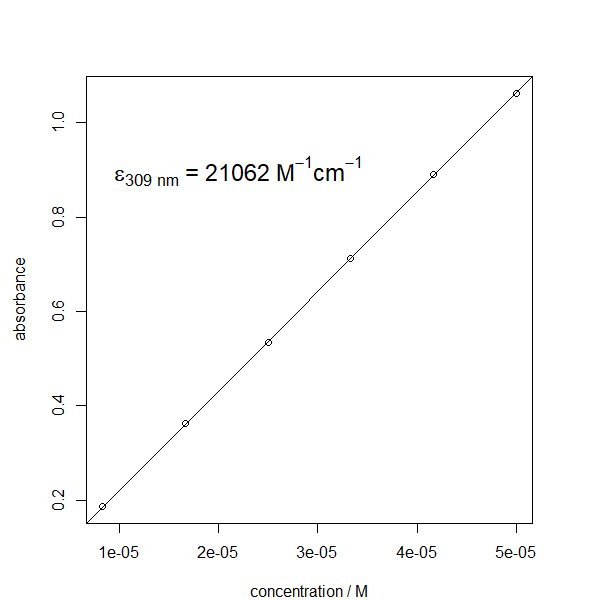
\includegraphics[width=0.5\linewidth]{Figures/ebshoe-calibration.png}
    \caption{Calibration curve for \refcmpd{ebs-rhs-ph}.}
    \label{fig:ebs-rhs-ph-calcurve}
\end{figure}

\subsection{Co-crystal structures}

\section{Conclusions}

\section{Experimental procedures}

\subsection{DNA titration procedure}
The following solutions were prepared:
\begin{itemize}
    \item Tris stock -- 1~\textsc{M}, pH 7.2
    \begin{itemize}
        \item 1.214~g tris(hydroxymethyl)aminomethane freebase
        \item 9~mL 1~\textsc{M} HCl
        \item dilute to 10~mL with water
    \end{itemize}
    \item EDTA$\cdot$\ce{2Na+} stock -- 0.1~\textsc{M}
    \begin{itemize}
        \item 372~mg EDTA$\cdot$\ce{2Na+}$\cdot$\ce{2H_2O}
        \item dilute to 10~mL with water
    \end{itemize}
    \item NaCl stock -- 1~\textsc{M}
    \begin{itemize}
        \item 584~mg NaCl
        \item dilute to 10~mL with water
    \end{itemize}
    \item T/E/N$\times$2 buffer
    \begin{itemize}
        \item 400~$\mu$L Tris stock -- final concentration 40~m\textsc{m}, pH 7.2
        \item 200~$\mu$L EDTA stock -- final concentration 2~m\textsc{m}
        \item 2~mL NaCl stock -- final concentration 200~m\textsc{m}
        \item 2~mL DMSO -- final concentration 20\% v/v
        \item dilute to 10~mL with water
    \end{itemize}
    \item T/E buffer
    \begin{itemize}
        \item 500~$\mu$L Tris stock -- final concentration 10~m\textsc{m}, pH 7.2
        \item 500~$\mu$L EDTA stock -- final concentration 2~m\textsc{m}
        \item dilute to 50~mL with water
    \end{itemize}
    \item TFA/M/W
    \begin{itemize}
        \item 10~$\mu$L TFA
        \item 4.5~mL methanol
        \item dilute to 10~mL with water
    \end{itemize}
    \item ct-DNA stock
    \begin{itemize}
        \item 30~mg ct-DNA
        \item 10~mL T/E buffer\footnote{The DNA can be cut into pieces using clean scissors, then magnetically stirred overnight to dissolve in the buffer. MW and viscosity can be reduced by drawing up rapidly through a 22G needle, then sonicating for up to 30~minutes. It is critical that the temperature remains below 30\degree C. The final concentration can be checked by diluting the stock solution fiftyfold and measuring the absorbance at 260~nm. An absorbance of 1.0 corresponds to a concentration of 75~$\mu$\textsc{m}bp.}
        % fiftyfold dilution 1.0898 at 260nm, 81.735uMbp
        % stock 4086.75uMbp
    \end{itemize}
    \item Ligand stock
\end{itemize}

\subsection{Synthetic methods}

Selenium was purified by refluxing in 32\% hydrochloric acid for 2~h, then washing with deionised water, methanol, then ether.

\subsubsection{Preparation of \refcmpd{ebs.h}.}
%TF-7-1B
Aqueous ammonia (30\% w/w, 637~$\mu$L, 10~mmol) was dissolved in anhydrous acetonitrile (5~mL), and to this was added a solution of dichloride \cmpd{dichloride} in acetonitrile (10~mL, 0.5~mmol/mL).
The solution was stirred at room temperature for 10~min, then the solvent was evaporated to give a cream powder which was used without further purification (858.4~mg, 87\%).

\ce{^{1}H} NMR (499~MHz, \ce{\emph{d}6}-DMSO) $\delta$ ppm 9.15 (1H, s), 8.05 (1H, d, \emph{J} = 8.04~Hz), 7.81 (1H, d, \emph{J} = 7.73~Hz), 7.66--7.55 (1H, m), 7.42 (1H, t, \emph{J} = 7.42~Hz).

MS (ESI +ve) m/z 199.9609 (\ce{MH+}) \ce{C7H6NOSe+} requires 199.9609 ($\Delta$=0~ppm).

\begin{figure}
    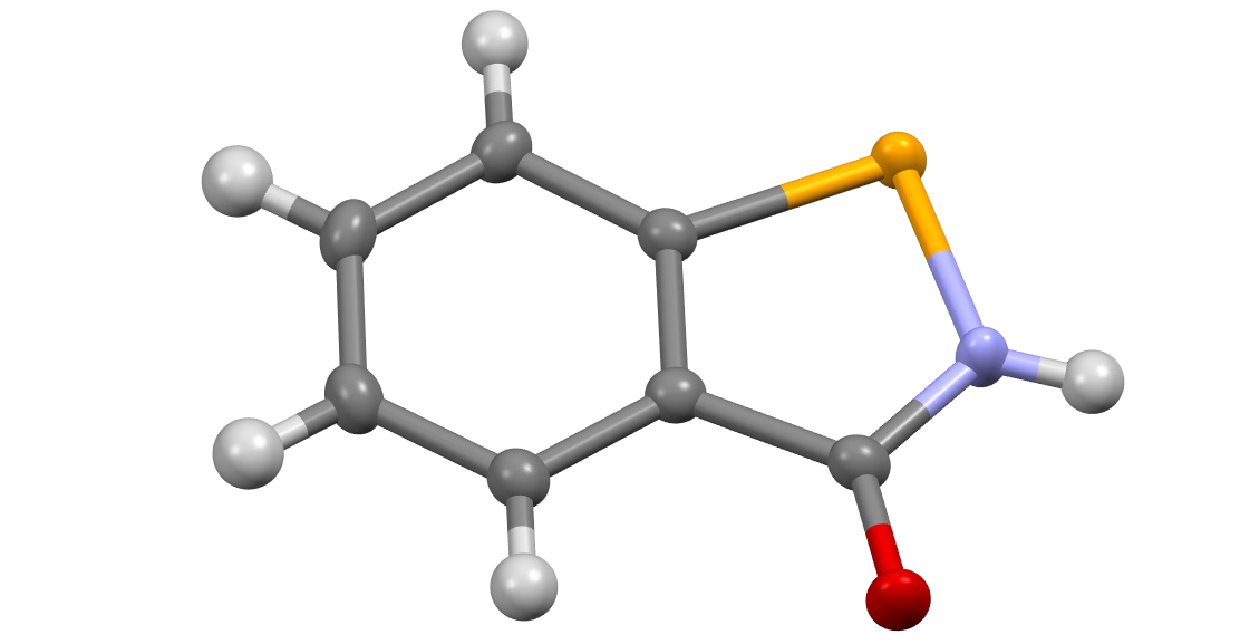
\includegraphics[width=0.8\linewidth]{Figures/ebs-h-xtal.pdf}
    \caption{X-ray crystal structure of \refcmpd{ebs.h}.}
\end{figure}

\subsubsection{Preparation of \refcmpd{ebs}\texorpdfstring{$\cdot$\textbf{S}}{.S}.}
%TF-7-12
To a sealed tube containing 4~\AA\ molecular sieves (740.7~mg) was added copper (I) iodide (34.3~mg, 0.180~mmol), DMEDA (27.6~mg, 31.3~mmol), potassium carbonate (305.3~mg, 2.209~mmol), benzisothiazolinone \cmpd{ebs}$\cdot$\textbf{S}, bromobenzene (190.6~mg, 1.213~mmol), and dioxane (3~mL).
The tube was capped and heated to 120\degree C for 18~h, then cooled and the mixture tipped into water (30~mL). The resulting blue suspension was centrifuged, and the blue supernatant discarded. The residue was dissolved in 1:1 DCM/methanol, and decanted off from the sieves.
The solvent was evaporated to afford a greenish solid, which was chromatographed to give the product as colourless needles (105.0~mg, 45\%).

\ce{^{1}H} NMR (400~MHz, \ce{\emph{d}6}-DMSO) $\delta$ ppm 8.05 (1H, d, \emph{J} = 8.2~Hz), 7.94 (1H, d, \emph{J} = 7.75~Hz), 7.75 (1H, t, \emph{J} = 7.69~Hz), 7.69 (2H, d, \emph{J} = 8.13~Hz), 7.56--7.46 (3H, m), 7.36 (1H, t, \emph{J} = 7.39~Hz).

MS (ESI +ve) m/z 228.0476 (\ce{MH+}) \ce{C13H10NOS+} requires 228.0478 ($\Delta$=0.88~ppm).

\subsubsection{Preparation of \refcmpd{bromodiamine}.}
The nitrobenzene (4.9982~g, 23.031~mmol) was dissolved in ethanol (35~mL), and to this was added tin (II) chloride dihydrate (26.022~g, 115.25~mmol, 5~eq).
The mixture was refluxed for 8~h, then cooled, concentrated, and diluted with water to a volume of 300~mL.
The thick white suspension was basified to pH 12, cooled again, and extracted with diethyl ether ($2\times200$~mL).
The combined organic layers were washed with brine (150~mL), dried (\ce{MgSO4}), and evaporated to give a brownish oil, which was triturated with petroleum ether to give a light yellow solid which was used without further purification (3.9759~g, 92\%).

\ce{^{1}H} NMR (400~MHz, \ce{\emph{d}6}-DMSO) $\delta$ ppm 6.6 (1H, d, \emph{J} = 2.17~Hz), 6.47--6.42 (1H, dd, \emph{J} = 2.17, 8.2~Hz), 6.39 (1H, d, \emph{J} = 8.2~Hz), 4.61 (4H, br. s).

\subsubsection{Preparation of \refcmpd{rhs-bromo-2py}.}
A 0.1~\textsc{m} solution of sodium methoxide was prepared by dissolving sodium metal (137~mg) in anhydrous methanol (50~mL).
Of this, 6.8~mL was added to 2-pyridine carbonitrile (714.0~mg, 6.858~mmol) and the mixture heated to 80\degree C under an argon atmosphere for 1~h to afford the carboximidate \cmpd{2py-carboximidate}.
To this was then added a solution of the diamine \cmpd{bromodiamine} (1.0226~g, 5.467~mmol) in a further 20~mL anhydrous methanol, followed by glacial acetic acid (650~$\mu$L, 11.5~mmol), and the mixture gently refluxed for 18~h.
Upon cooling, the mixture was concentrated to give a yellow oil which was triturated with 1~\textsc{m} aqueous ammonia to give a friable pale yellow solid, which was washed with water to give the product (1.3595~g, 91\%).

\ce{^{1}H} NMR (400~MHz, \ce{\emph{d}6}-DMSO + \textit{d}-TFA vapour) $\delta$ ppm 8.72 (1H, d, \emph{J} = 4.21~Hz), 8.31 (1H, d, \emph{J} = 7.85~Hz), 8.01 (1H, t, \emph{J} = 7.7~Hz), 7.79 (1H, s), 7.63--7.49 (2H, m), 7.37 (1H, d, \emph{J} = 8.53~Hz).

MS (ESI +ve) m/z 273.9975 (\ce{MH+}) \ce{C12H9BrN3+} requires 273.9974 ($\Delta$=0.36~ppm).

\subsubsection{Preparation of \refcmpd{rhs-bromo-2py.pmb}.}
The benzimidazole \cmpd{rhs-bromo-2py} (1034.1~mg, 3.797~mmol) and sodium hydride (60\% in oil, 298.2~mg, 7.450~mmol, 2.5~eq) were dissolved in anhydrous DMF (6~mL) at 0\degree C, and to this was added \textit{p}-methoxybenzyl chloride (600~$\mu$L, 4.42~mmol, 1.2~eq).
The mixture was warmed to room temperature and stirred for 18~h, then diluted with water (50~mL) and extracted with DCM ($2\times80$~mL).
The combined organic phases were washed with brine, dried (\ce{MgSO4}) and evaporated to give a yellow oil, which was chromatographed to afford two major fractions:
\begin{enumerate}
    \item 633~mg
    \item 591~mg
\end{enumerate}
which when combined gave a 82\% overall yield.

\ce{^{1}H} NMR (499~MHz, \ce{CDCl3}) $\delta$ ppm 8.67 (1H, d, \emph{J} = 4.12~Hz), 8.4 (1H, d, \emph{J} = 7.95~Hz), 7.98 (1H, d, \emph{J} = 1.52~Hz), 7.86 (1H, dt, \emph{J}\textsubscript{1} = 1.65~Hz, \emph{J}\textsubscript{2} = 7.78~Hz), 7.38--7.34 (2H, m), 7.23 (1H, d, \emph{J} = 8.63~Hz), 7.11 (2H, d, \emph{J} = 8.65~Hz), 6.78 (2H, d, \emph{J} = 8.65~Hz), 6.08 (2H, s), 3.73 (3H, s).

MS (ESI +ve) m/z 394.0555 (\ce{MH+}) \ce{C20H17BrN3O+} requires 394.0550 ($\Delta$=1.27~ppm).

\begin{figure}
    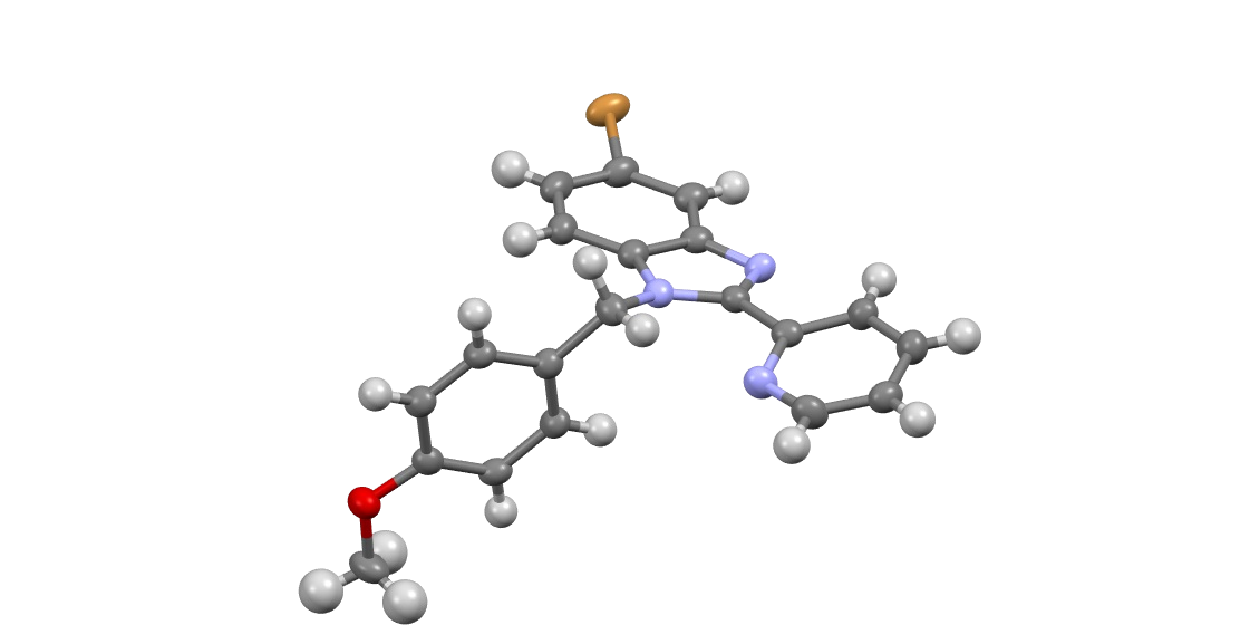
\includegraphics[width=0.8\linewidth]{Figures/rhs-bromo-2py-pmb-xtal.pdf}
    \caption{X-ray crystal structure of \refcmpd{rhs-bromo-2py.pmb}.}
\end{figure}

\subsubsection{Preparation of \refcmpd{rhs-bromo-ph}.}
Sodium metabisulfite (9.670~g, 50.85~mmol) was dissolved in 50~mL water and added to 200~mL ethanol, then benzaldehyde (5.444~g, 51.30~mmol) was added.
This was stirred at room temperature for 1~h, then a solution of the diamine \cmpd{bromodiamine} (4.0437~g, 21.6~mmol) in ethanol (40~mL) was added, and the mixture refluxed under nitrogen for 24~, then cooled and left to stand for 60~h.
The solvent was removed by rotary evaporator, and the residue triturated with 1~\textsc{m} aqueous ammonia (50~mL). 
The resulting precipitate was filtered off, washed with water ($2\times25$~mL), cold diethyl ether (5~mL), and dried affording the benzimidazole \cmpd{rhs-bromo-ph} (5.1646~g, 79\%).

\ce{^{1}H} NMR (499~MHz, \ce{\emph{d}6}-DMSO + \textit{d}-TFA) $\delta$ ppm 8.18 (2H, d, \emph{J} = 6.89~Hz), 7.83 (1H, s), 7.64--7.52 (4H, m), 7.41 (1H, dd, \emph{J}\textsubscript{1} = 1.51~Hz, \emph{J}\textsubscript{2} = 8.52~Hz).

\subsubsection{Preparation of \texorpdfstring{\refcmpd{ebs-rhs-ph.pmb}$\cdot$\textbf{S}}{\refcmpd{ebs-rhs-ph.pmb}.S}.}
Benzisothiazolinone \cmpd{ebs.h}$\cdot$\textbf{S} (173.1~mg, 1.142~mmol), aryl bromide \cmpd{rhs-bromo-ph.pmb} (401.9~mg, 1.022~mmol), 4~\AA\ molecular sieves (607.1~mg), DMEDA (32.7~mg, 0.371~mmol), potassium carbonate (283.8~mg, 2.053~mmol), and dioxane (3~mL) were combined in a sealed tube under a nitrogen atmosphere, and heated at 120\degree C for 24~h.
The mixture was then cooled to room temperature and tipped into water (40~mL).
The suspension was centrifuged, and the supernatant discarded, then the residue redissolved in methanol ($2\times40$~mL).
This was filtered, and the filtrate evaporated to give a light brown oil, which was applied to a SNAP 25~g silica cartridge and eluted with an ethyl acetate/petroleum ether gradient to give two fractions:
\begin{enumerate}
    \item 160.9~mg, aryl bromide \cmpd{rhs-bromo-ph.pmb},
    \item 231.2~mg, 48\%, benzisothiazolinone-benzimidazole \cmpd{ebs-rhs-ph.pmb}$\cdot$\textbf{S}.
\end{enumerate}

\cmpd{ebs-rhs-ph.pmb}$\cdot$\textbf{S} crystallised in two distinct polymorphs:
\begin{enumerate}
    \item P$\bar{1}$, m.p. 101.0--104.2\degree C
    \item P$2_1$/n, m.p. 134.1--138.4\degree C
\end{enumerate}

\ce{^{1}H} NMR (600~MHz, \ce{\emph{d}6}-DMSO) $\delta$ ppm 8.03 (1H, d, \emph{J} = 8.08~Hz), 7.92 (1H, d, \emph{J} = 7.67~Hz), 7.86--7.79 (2H, m), 7.73 (3H, d, \emph{J} = 4.68~Hz), 7.55 (3H, d, \emph{J} = 3.42~Hz), 7.51--7.44 (2H, m), 6.93 (2H, d, \emph{J} = 8.38~Hz), 6.82 (2H, d, \emph{J} = 8.46~Hz), 5.52 (2H, s), 3.66 (3H, s).

MS (ESI +ve) m/z 464.1431 (\ce{MH+}) \ce{C28H22N3O2S+} requires 464.1427 ($\Delta$=0.86~ppm).

\subsubsection[Preparation of \refcmpd{rhs-nitro-amide}]{Preparation of N-(2-amino-5-nitrophenyl)benzamide \refcmpd{rhs-nitro-amide}}
4-Nitro-1,2-benzenediamine (3.0797~g, 20.110~mmol) and TEA (3~mL, distilled from \ce{CaH2}) were dissolved in anhydrous THF (150~mL).
Benzoyl chloride (1.5~mL, 1.8~g, 13~mmol) was then added at $-10$\degree C and the mixture slowly warmed to room temperature while stirring for 18~h.
The mixture was then tipped into water (400~mL), and extracted with ethyl acetate ($3\times100$~mL).
The combined organic layers were washed with water ($2\times200$~mL), brine (200~mL), then dried (\ce{MgSO4}) and evaporated to give a reddish solid.
This was recrystallised from ethyl acetate to give the amide \cmpd{rhs-nitro-amide} as yellow crystals (2.5027~g, 75\%).

\ce{^1H} NMR (400~MHz, DMSO-\emph{d6}) $\delta$ 9.66 (s, 1H), 8.04 (s, 1H), 7.92 (d, J = 7.4 Hz, 2H), 7.83 (d, J = 9.2 Hz, 1H), 7.50 (d, J = 6.8 Hz, 1H), 7.44 (t, J = 7.3 Hz, 2H), 6.71 (d, J = 9.0 Hz, 1H), 6.52 (s, 2H).

\subsubsection[Preparation of \refcmpd{rhs-nitro}]{Preparation of 6-nitro-2-phenyl-1\emph{H}-benzo[\emph{d}]imidazole \refcmpd{rhs-nitro}}
%TF-7-94-CP
Amide \cmpd{rhs-nitro-amide} (1.2283~g, 4.7749~mmol) was refluxed in a solution of \ce{BF3\cdot OEt2} (0.75~mL) and dioxane (75~mL) for 1.5~h.
The mixture was then cooled to room temperature, stirred for 18~h, then heated to reflux again for 2~h.
The yellow solution was diluted with water (300~mL) and extracted with ethyl acetate ($3\times75$~mL),
The combined organic layers were washed with water and brine (100~mL each), then dried (\ce{Na2SO4}), and evaporated to give a brown oil.
Trituration with petroleum spirit/dichloromethane afforded \cmpd{rhs-nitro} as a light brown friable solid (1.0606~g, 93\%).

\ce{^1H} NMR (400~MHz, DMSO-\emph{d6} + \textit{d}-TFA) $\delta$ 8.47 (s, 1H), 8.21 (q, J = 3.2 Hz, 2H), 8.13 (q, J = 3.7 Hz, 1H), 7.76 (d, J = 8.9 Hz, 1H), 7.54--7.62 (m, 3H).

MS (ESI +ve) m/z 240.0768 (\ce{MH+}) \ce{C13H10N3O2+} requires 240.0768 ($\Delta$=0~ppm).

\begin{figure}[ht]
    \centering
    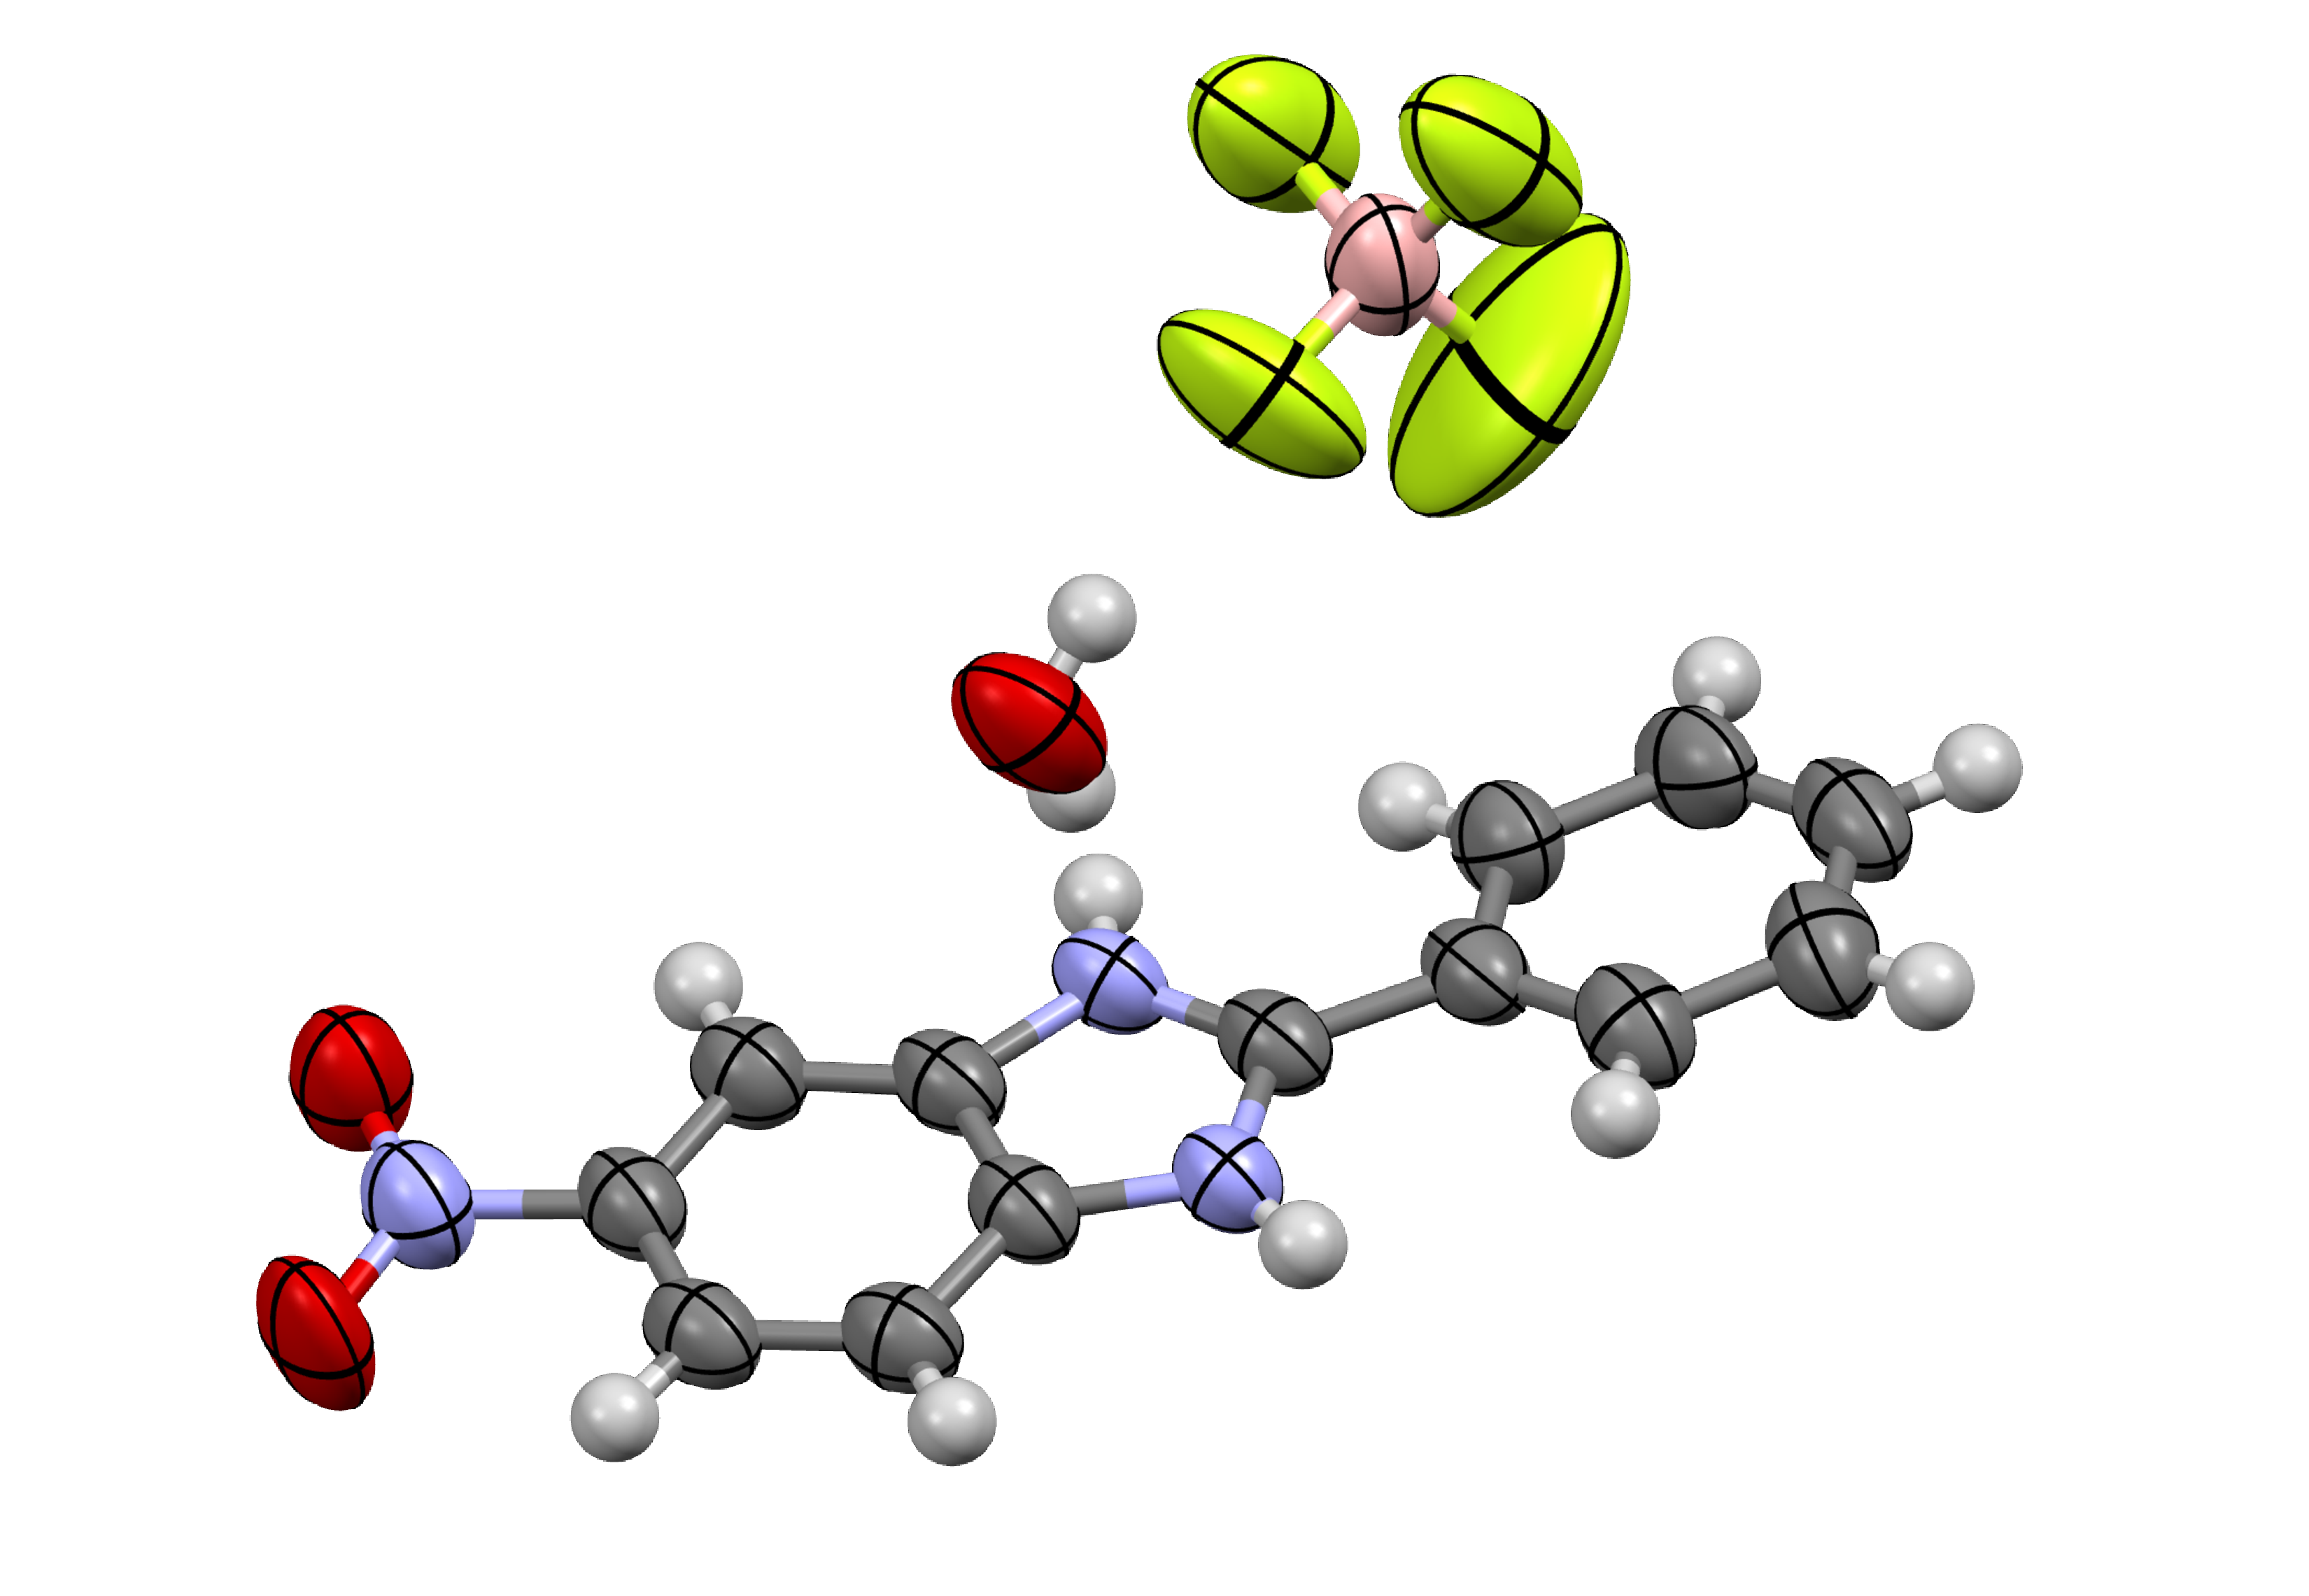
\includegraphics[width=0.8\linewidth]{Figures/rhs-nitro-xray.pdf}
    \caption{X-ray crystal structure of \refcmpd{rhs-nitro} as the tetrafluoroborate salt.}
    \label{fig:rhs-nitro-xray}
\end{figure}

\subsubsection[Preparation of \refcmpd{rhs-amine}]{Preparation of 2-phenyl-1\emph{H}-benzo[\emph{d}]imidazol-6-amine \refcmpd{rhs-amine}}
%TF-7-117-CP
A solution of the nitrobenzene \cmpd{rhs-nitro} (893.6~mg, 3.735~mmol) and tin (II) chloride dihydrate (4.410~g, 19.54~mmol) in concentrated hydrochloric acid (20~mL) was refluxed for 2~h.
The solution was then cooled, and basified to pH 10 using 5~M aqueous sodium hydroxide.
This was then extracted with ethyl acetate ($2\times30$~mL), washing with water and brine (30~mL each).
The combined organic layers were dried (\ce{Na2SO4}) then evaporated to give \cmpd{rhs-amine} as a brownish solid (677.2~mg, 87\%).

\ce{^{1}H} NMR (400~MHz, \ce{\emph{d}6}-DMSO + \textit{d}-TFA) $\delta$ ppm 8.2--8.01 (1H, m), 7.64 (1H, d, \emph{J} = 6.54~Hz), 7.53 (1H, d, \emph{J} = 8.66~Hz), 7.07 (0H, s), 6.94 (0H, d, \emph{J} = 8.59~Hz).

MS (ESI +ve) m/z 210.1026 (\ce{MH+}) \ce{C13H12N3+} requires 210.1026 ($\Delta$=0~ppm).

\begin{figure}[ht]
    \centering
    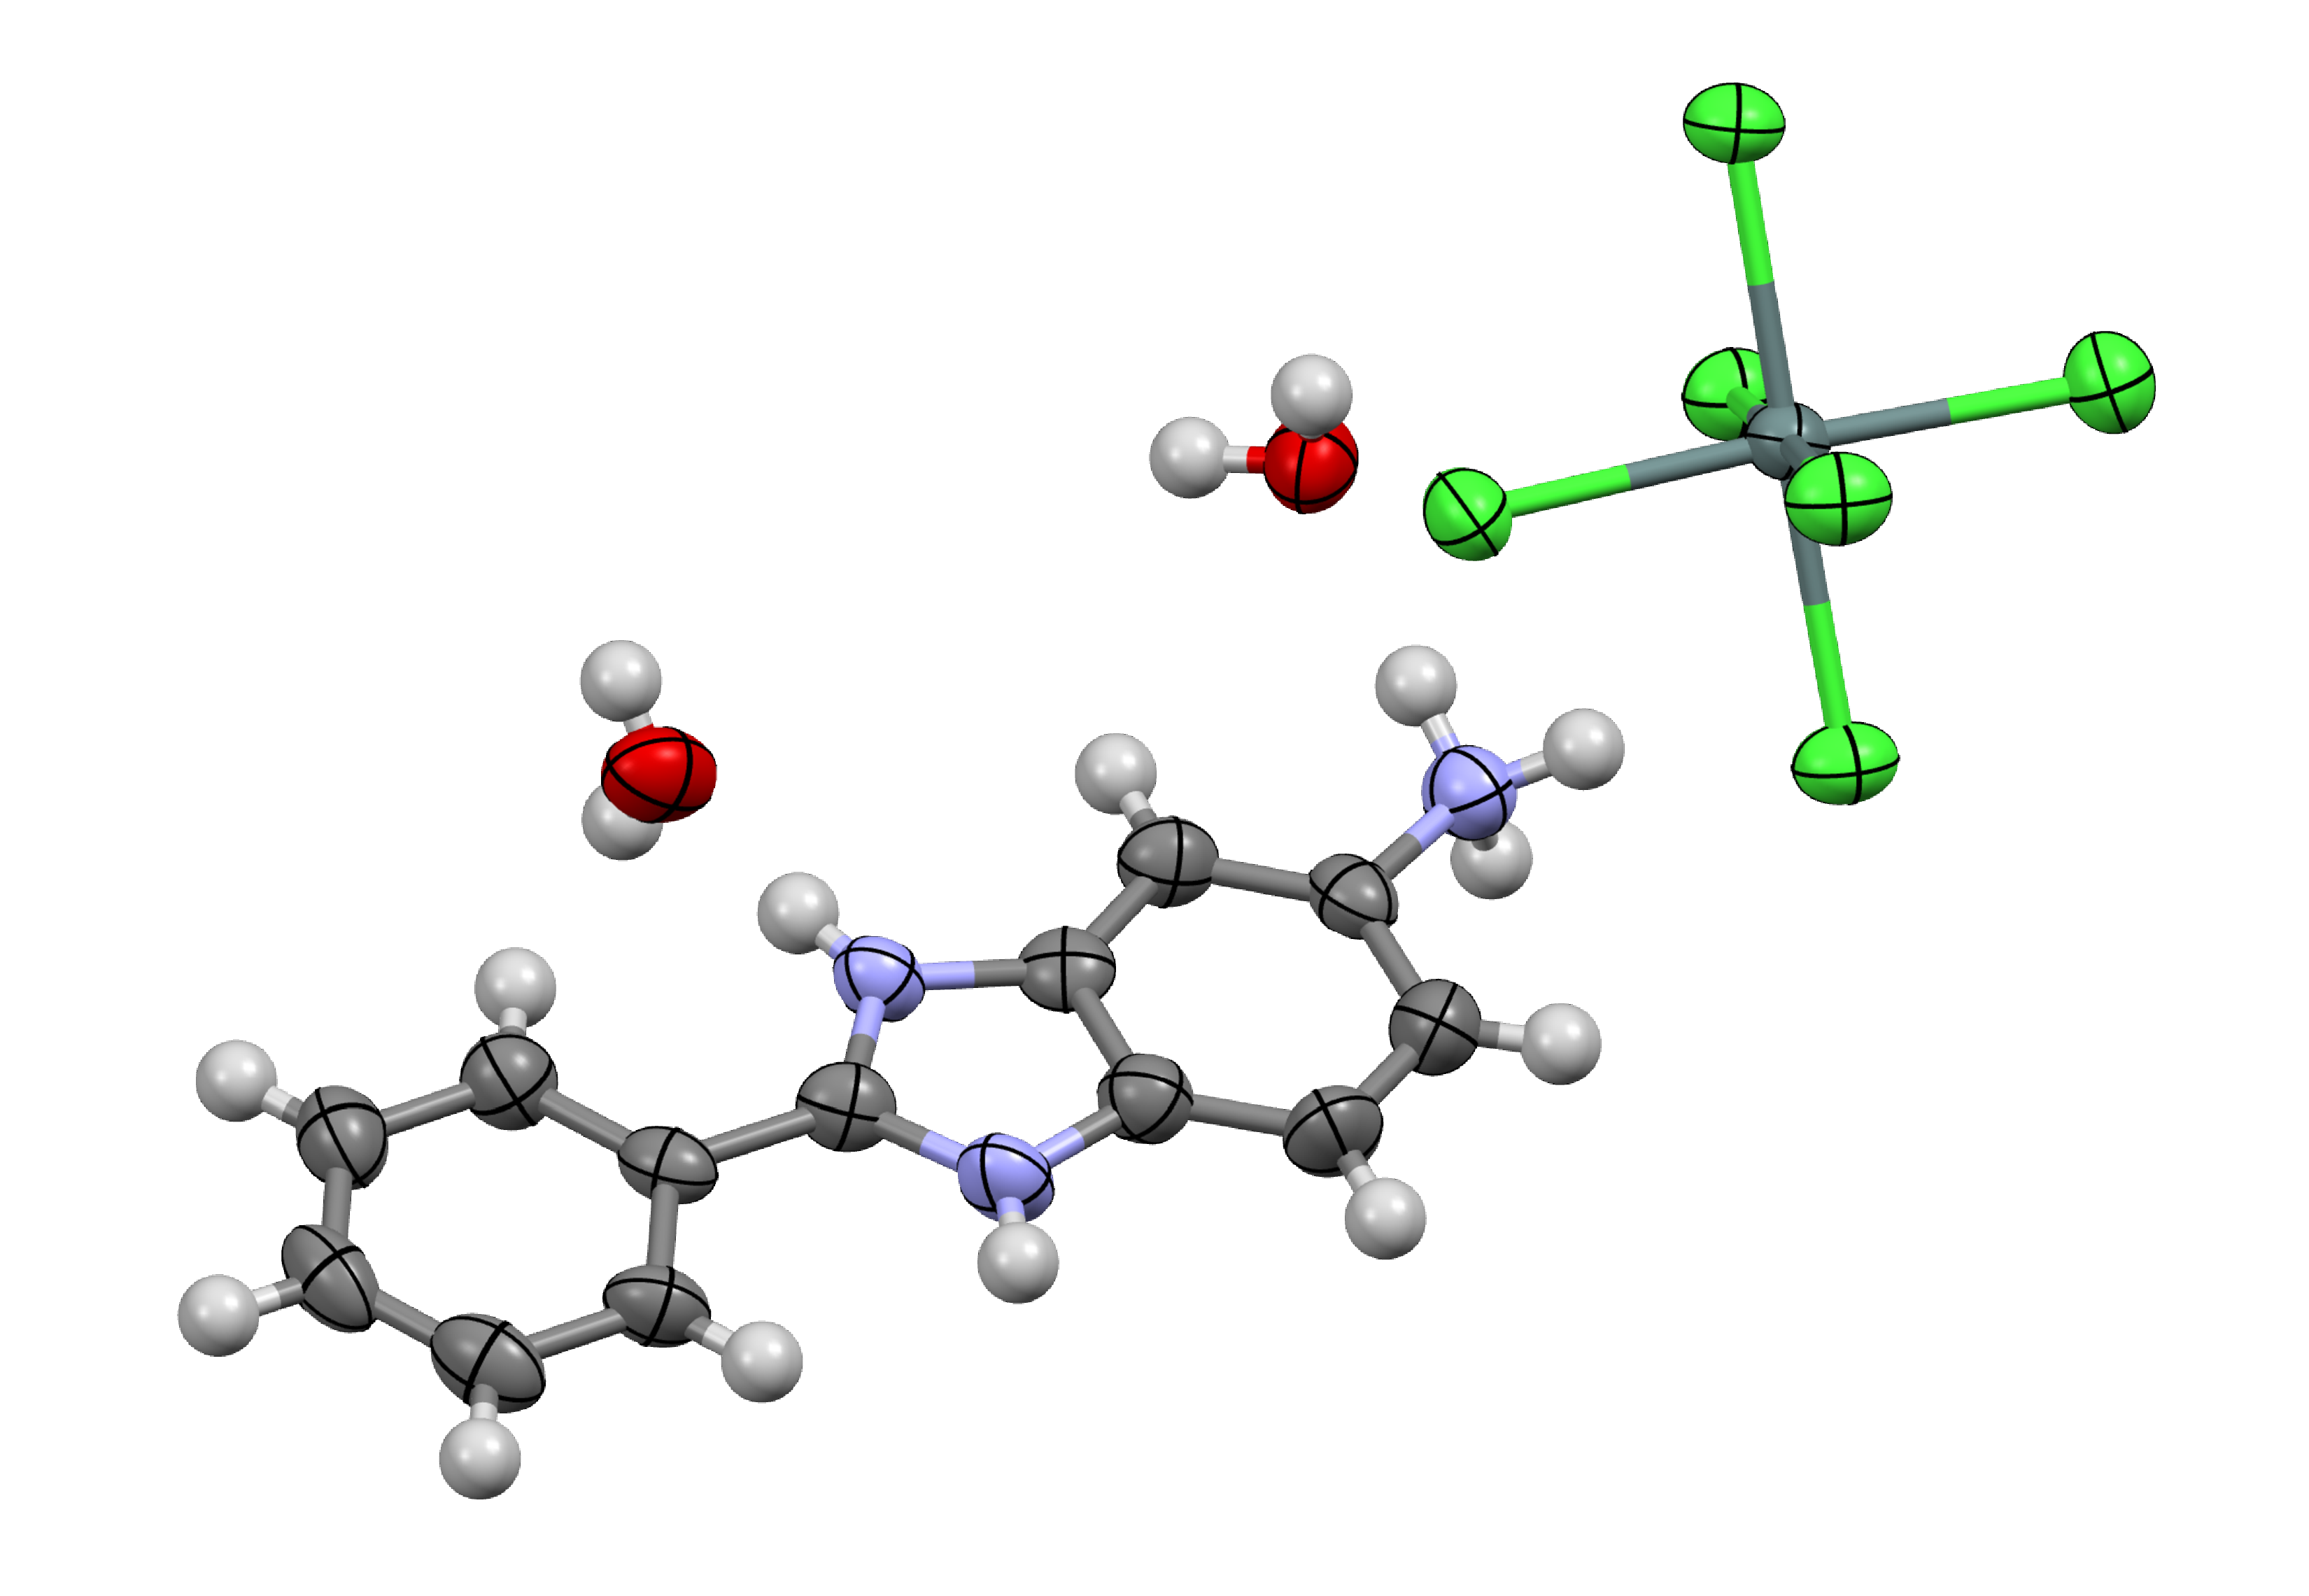
\includegraphics[width=0.8\linewidth]{Figures/rhs-amine-xray.pdf}
    \caption{X-ray crystal structure of \refcmpd{rhs-amine} as the hexachlorostannate salt.}
    \label{fig:rhs-amine-xray}
\end{figure}

\subsubsection[Preparation of \refcmpd{ebs-rhs-ph}]{Preparation of 2-(2-phenyl-1\emph{H}-benzo[\emph{d}]imidazol-6-yl)benzo[\emph{d}][1,2]\-selenazol-3(2\emph{H})-one \refcmpd{ebs-rhs-ph}}
%TF-7-188-C1F1
Diselenide \cmpd{diselenide} (440.1~mg, 1.100~mmol) was refluxed in thionyl chloride with 2 drops DMF for 2~h.
The excess reagent was removed by vacuum distillation, and the residue was dissolved in anhydrous acetonitrile (10~mL).
This was added dropwise to a solution of the aniline \cmpd{rhs-amine} (440.4~mg, 2.105~mmol) and TEA (2~mL) in a further 10~mL anhydrous acetonitrile.
The mixture was stirred at room temperature for 18~h, then briefly brought to reflux.
It was then cooled, diluted with water (30~mL) and extracted into ethyl acetate ($3\times50$~mL).
The combined organic layers were washed with water and brine (50~mL each), then dried (\ce{MgSO4}), then evaporated onto celite.
This was chromatographed on a SNAP 25~g silica cartridge using an ethyl acetate/methanol gradient, affording 2 major fractions:
\begin{enumerate}
    \item orange solid, 67.7~mg, 8\%, \cmpd{ebs-rhs-ph}, m.p. 170\degree C (dec.)
    \item yellow solid, 166.0~mg, 38\%, starting material \cmpd{rhs-amine}
\end{enumerate}

\ce{^{1}H} NMR (499~MHz, \ce{\emph{d}6}-DMSO) $\delta$ ppm 8.23--8.17 (2H, m), 8.12 (1H, d, \emph{J} = 8.08~Hz), 8.07 (1H, s), 7.94 (1H, d, \emph{J} = 7.64~Hz), 7.83 (1H, d, \emph{J} = 8.66~Hz), 7.76--7.67 (4H, m), 7.63 (1H, d, \emph{J} = 8.63~Hz), 7.51 (1H, t, \emph{J} = 7.34~Hz).

MS (ESI +ve) m/z 392.0298 (\ce{MH+}) \ce{C20H14N3OSe+} requires 392.0297 ($\Delta$=0.26~ppm).

\begin{comment}
\subsubsection{Preparation of 2-chloro-4-nitro-\emph{N}-phenylbenzamide \refcmpd{2cl-4no2-amide}}
%TF-7-128-recryst
2-Chloro-4-nitrobenzoic acid (10.3144~g, 51.173~mmol) was refluxed in thionyl chloride (20~mL) with 3 drops DMF for 2~h.
The excess reagent was then removed by vacuum distillation and the residue was dissolved in anhydrous DCM (100~mL).
This was added slowly to a solution of aniline (4.756~g, 51.07~mmol) and TEA (10~mL, distilled from \ce{CaH2}) in a further 100~mL of anhydrous DCM.
The mixture was stirred for 18~h at room temperature, then the solvent was removed \emph{in vacuo}.
The residue was washed with water ($3\times$50~mL), then recrystallised from ethanol to afford \cmpd{2cl-4no2-amide} as colourless plates (10.5134~g, 75\%).

\ce{^{1}H} NMR (500~MHz, \ce{CDCl3}) $\delta$ ppm
7.23 (t, J=7.48 Hz, 1 H),
7.42 (t, J=7.78 Hz, 2 H),
7.64 (d, J=7.93 Hz, 2 H),
7.81 (br. s., 1 H),
7.93 (d, J=8.39 Hz, 1 H),
8.24 (d, J=8.39 Hz, 1 H),
8.35 (d, J=1.07 Hz, 1 H).

\subsubsection[Preparation of \refcmpd{ebs-3no2}]{Preparation of 6-nitro-2-phenylbenzo[\emph{d}][1,2]selenazol-3(2\emph{H})-one \refcmpd{ebs-3no2}}
Copper (I) iodide (127.2~mg, 0.6679~mmol) and 1,10-phenanthroline (121.5~mg, 0.6743~mmol) were dissolved in anhydrous DMF (4~mL).
To this was added selenium (1035.1~mg, 13.109~mmol) and potasssium carbonate (755.9~mg, 5.469~mmol), and the mixture heated to 120\degree C under a nitrogen atomsphere for 5~min.
The mixture was then cooled, the amide \cmpd{2cl-4no2-amide} (968.4~mg, 3.500~mmol) added, and the mixture was again heated at 120\degree C under nitrogen for 18~h.
Upon cooling, the mixture was tipped into brine (200~mL) and stirred in the air for 3~h, then extracted into ethyl acetate ($4\times50$~mL).
The combined organic phases were washed with water then brine (100~mL each), then dried (\ce{MgSO4}) and evaporated to give a dark orange solid.
This was redissolved in ethanol (70~mL) and cooled to $-20$\degree C for 72~h, affording \cmpd{ebs-3no2} as an orange precipitate, which was filtered and dried (119.1~mg, 11\%, m.p. 256.2--258.2\degree C (dec.)).
The mother liquor was loaded onto silica and chromatographed using a SNAP 50~g silica cartridge, affording 3 major fractions which were not further characterised.

{\footnotesize
\ce{^{1}H} NMR (400~MHz, \ce{\emph{d}6}-DMSO) $\delta$ ppm
.

\ce{^{13}C} NMR (100~MHz, \ce{\emph{d}6}-DMSO) $\delta$ ppm
.

\ce{^{77}Se} NMR (0~MHz, \ce{\emph{d}6}-DMSO) $\delta$ ppm
.

MS (ESI +ve) m/z 320.97720 (\ce{MH+}) \ce{C13H9N2O3Se+} requires 320.97729 ($\Delta$=-0.09~mmu).
}

\begin{figure}[ht]
    \centering
    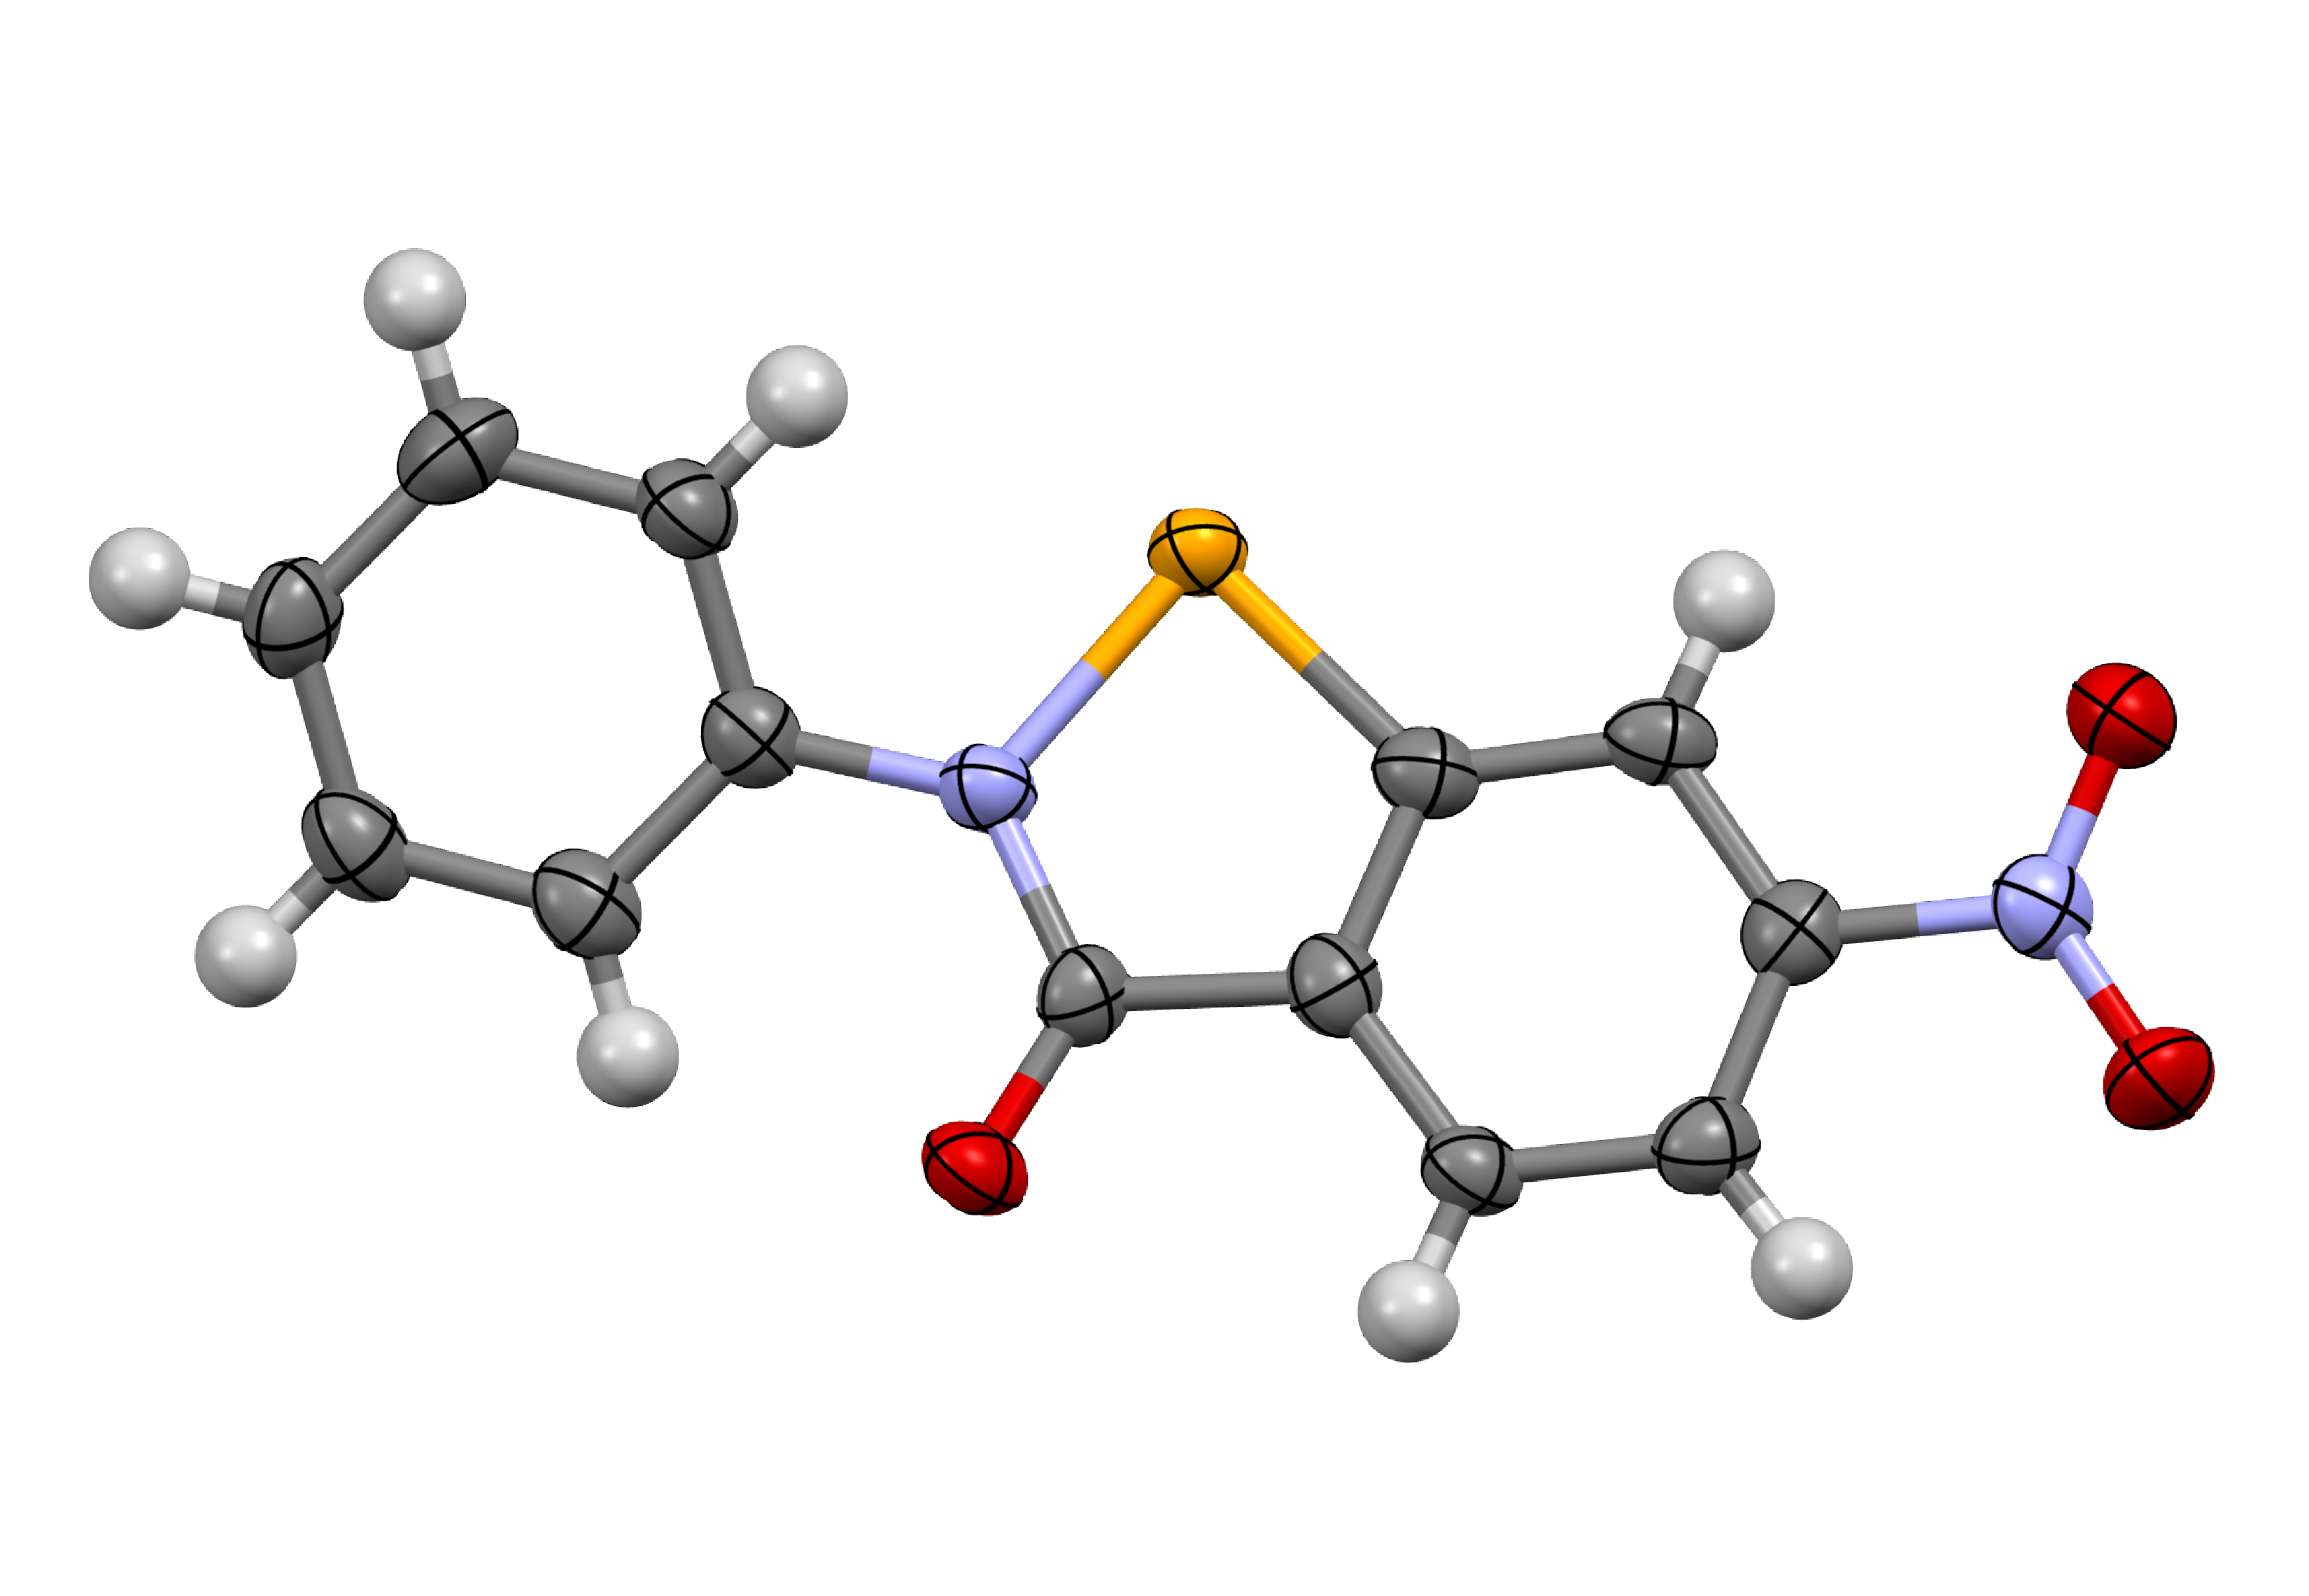
\includegraphics[width=0.8\linewidth]{Figures/ebs-3no2-xray.pdf}
    \caption{X-ray crystal structure of \refcmpd{ebs-3no2}.}
    \label{fig:ebs-3no2-xray}
\end{figure}
\end{comment}

\subsubsection[Preparation of \refcmpd{ebs-3no2-4nh2}]{Preparation of 2-(4-amino-3-nitrophenyl)benzo[\emph{d}][1,2]selenazol-3(2\emph{H})-one \refcmpd{ebs-3no2-4nh2}}
Diselenide \cmpd{diselenide} (1.2025~g, 3.005~mmol) was dissolved in thionyl chloride (20~mL) and refluxed for 30~minutes, and the colour changed from purple to light yellow.
Excess thionyl chloride was removed \emph{in vacuo}, and the residue dissolved in anhydrous THF (50~mL).
To this was added a solution of 2-nitro-1,4-phenylenediamine (991.9~mg, 6.477~mmol) and triethylamine (3~mL, dist. from \ce{CaH2}) in anhydrous THF (50~mL).
This mixture was stirred at room temperature for 18~h, then filtered, washing the precipitate with water, to afford 2-(4-amino-3-nitrophenyl)benzo[\emph{d}][1,2]selenazol-3(2\emph{H})-one \cmpd{ebs-3no2-4nh2} as a brick red solid (940~mg, 61\%, m.p. (DMF) 300.8--302.0~\degree~C).


\ce{^{1}H} NMR (400~MHz, \ce{\emph{d}6}-DMSO) $\delta$ ppm
7.08 (d, \emph{J}=9.00~Hz, 1 H),
7.46 (t, \emph{J}=7.43~Hz, 1 H),
7.55 (s, 2 H),
7.59--7.70 (m, 2 H),
7.86 (d, \emph{J}=7.43~Hz, 1 H),
8.06 (d, \emph{J}=7.83~Hz, 1 H),
8.12 (d, \emph{J}=1.96~Hz, 1 H).

\ce{^{13}C} NMR (100~MHz, \ce{\emph{d}6}-DMSO) $\delta$ ppm
120.29 (s),
121.49 (s),
126.32 (s),
126.71 (s),
127.77 (s),
128.31 (s),
128.45 (s),
129.68 (s),
132.66 (s),
134.13 (s),
139.33 (s),
145.03 (s),
165.70 (s).

MS (ESI +ve) m/z 335.9882 (\ce{MH+}) \ce{C13H10N3O3Se+} requires 335.9881 ($\Delta$=0.298~ppm).

\subsubsection[Preparation of \refcmpd{ebs-3no2-4nh-2py}]{Preparation of \emph{N}-(2-nitro-4-(3-oxobenzo[\emph{d}][1,2]selenazol-2(3\emph{H})-yl)phenyl) picolinamide \refcmpd{ebs-3no2-4nh-2py}}
Picolinic acid (256.6~mg, 2.084~mmol) was dissolved in anhydrous THF (5~mL) and triethylamine (1~mL, dist. from \ce{CaH2}), then trichlorobenzoyl chloride (325~uL) was added and the mixture stirred for 10~minutes.
The nitroaniline \cmpd{ebs-3no2-4nh2} (242.8~mg, 0.956~mmol) was then added, and the mixture stirred under argon for 24~h, during which time the dark red colour faded to give a yellow solution.
The mixture was tipped into water (100~mL) and filtered to afford a yellow precipitate, which was recrystallised from pyridine (50~mL) to give 2-(4-amino-3-nitrophenyl)benzo[\emph{d}][1,2]selenazol-3(2\emph{H})-one \cmpd{ebs-3no2-4nh-2py} as a yellow solid (93.2~mg, 20\%, m.p. 342.7--343.7~\degree~C).

\ce{^{1}H} NMR (500~MHz, \ce{\emph{d}6}-DMSO) $\delta$ ppm
7.51 (t, \emph{J}=7.40~Hz, 1 H)
7.66--7.83 (m, 1 H)
7.94 (d, \emph{J}=7.63~Hz, 1 H)
8.04 (dd, \emph{J}=9.00, 2.40~Hz, 1 H)
8.09--8.17 (m, 2 H)
8.23 (d, \emph{J}=7.78~Hz, 1 H)
8.68 (d, \emph{J}=2.44~Hz, 1 H)
8.73 (d, \emph{J}=9.00~Hz, 1 H)
8.81 (d, \emph{J}=4.43~Hz, 1 H)
12.22 (s, 1 H)

MS (ESI +ve) m/z 441.0100 (\ce{MH+}) \ce{C19H13N4O4Se+} requires 441.0096 ($\Delta$=0.907~ppm).

\begin{comment}
\subsubsection{Preparation of 2-iodobenzoic anhydride \refcmpd{2-iodobenzoicanhydride}}
2-Iodobenzoic acid (1.9957~g, 8.045~mmol) and DCC (0.8457~g, 4.098~mmol) were stirred in anhydrous diethyl ether (10~mL) for 18~h. The white precipitate was filtered off, washing with cold anhydrous ether ($2\times$10~mL). The filtrate was concentrated \emph{in vacuo} to afford 2-iodobenzoic anhydride \cmpd{2-iodobenzoicanhydride} as an off-white solid (1.9623~g, 100\%).

\subsubsection{Preparation of \emph{N}-(3,4-dinitrophenyl)-2-iodobenzamide \refcmpd{iodoamide-3no2-4no2}}
A neat mixture 2-iodobenzoic anhydride \cmpd{2-iodobenzoicanhydride} (1.9226~g, 4.022~mmol), 3,4-dinitroaniline (0.7290~g, 3.981~mmol) and zinc iodide (0.2140~g, 0.673~mmol) was stirred at 80~\degree~C under an argon atmosphere.
The melt was cooled to room temperature, dissolved in diethyl ether (40~mL), and the solution washed with 1~\textsc{m} \ce{HCl} (20~mL), 0.8~\textsc{m} sodium bicarbonate solution (50~mL), then brine (50~mL).
The organic phase was dried (\ce{MgSO4}), then evaporated to afford a yellow oil.
This was triturated with petroleum ether (5~mL) with a few drops of dichloromethane to afford \emph{N}-(3,4-dinitrophenyl)-2-iodobenzamide \cmpd{iodoamide-3no2-4no2} as an off white solid (0.926~g, 56\%, m.p. XXX--XXX).\autocite{Shivani2007}

\ce{^{1}H} NMR (400~MHz, \ce{\emph{d}6}-DMSO) $\delta$ ppm
7.28 (td, \emph{J}=7.20, 1.96~Hz, 1 H),
7.48--7.61 (m, 2 H),
7.97 (d, \emph{J}=7.83~Hz, 1 H),
8.07 (dd, \emph{J}=8.80, 1.37~Hz, 1 H),
8.30 (d, \emph{J}=8.61~Hz, 1 H),
8.47 (d, \emph{J}=1.17~Hz, 1 H),
11.40 (s, 1 H).

\ce{^{13}C} NMR (100~MHz, \ce{\emph{d}6}-DMSO) $\delta$ ppm
93.91 (s),
115.06 (s),
122.90 (s),
127.96 (s),
128.72 (s),
128.76 (s),
132.28 (s),
136.30 (s),
139.69 (s),
142.03 (s),
144.21 (s),
144.76 (s),
168.92 (s).

MS (ESI +ve) m/z ??? (\ce{MH+}) \ce{C13H9IN3O5+} requires 413.9581 ($\Delta$=0~ppm).

\subsubsection{Preparation of 6-bromo-2-phenyl-1\textbf{H}-benzo[\emph{d}]imidazole}
\end{comment}

\printbibliography[heading=subbibliography]
\end{refsection}
